% Header mit Deklarationen
\documentclass[%
	latex,%              PDFTex verwenden
	a4paper,%             A4 Papier
	oneside,%             Einseitig
	chapterprefix,%       Kapitel anschreiben als Kapitel
	headsepline,%         Linie nach Kopfzeile
	%footsepline,%         Linie vor Fusszeile
	%pointlessnumbers,%     Nummern ohne abschließenden Punkt
	12pt%                 Grössere Schrift, besser lesbar am bildschrim
]{scrbook}
%
% Paket für Übersetzungen ins Deutsche
%
% \usepackage[french,ngerman]{babel}

\usepackage{todonotes}
\usepackage{multirow}

\usepackage{tikz}

\usetikzlibrary{%
  arrows,%
  shapes.misc,% wg. rounded rectangle
  shapes.arrows,%
  chains,%
  matrix,%
  positioning,% wg. " of "
  scopes,%
  decorations.pathmorphing,% /pgf/decoration/random steps | erste Graphik
  shadows,%
  trees%
}

%
% Pakete um Latin1 Zeichnensätze verwenden zu können und die dazu
% passenden Schriften.
%
\usepackage[latin1]{inputenc}
\usepackage[T1]{fontenc}

%
% Paket zum Erweitern der Tabelleneigenschaften
%
\usepackage{array}

%
% Paket für schönere Tabellen
%
\usepackage{booktabs}

%
% Paket um Grafiken einbetten zu können
%
\usepackage{graphicx} 
%
% Spezielle Schrift im Koma-Script setzen.
%
\usepackage{titlesec}
\newcommand*{\justifyheading}{\raggedleft}
\titleformat{\chapter}[display]
  {\normalfont\Huge\bfseries\justifyheading}{\thechapter}
  {10pt}{\Huge}
\titleformat{\section}
  {\normalfont\Large\bfseries}{\thesection}{1em}{}
\titleformat{\subsection}
  {\normalfont\large\bfseries}{\thesubsection}{1em}{}
% \setkomafont{sectioning}{\normalfont\bfseries}
\setkomafont{captionlabel}{\normalfont\bfseries} 
\setkomafont{pagehead}{\normalfont\bfseries} % Kopfzeilenschrift
\setkomafont{descriptionlabel}{\normalfont\bfseries}

%
% Zeilenumbruch bei Bildbeschreibungen.
%
\setcapindent{1em}

%
% Kopf und Fußzeilen
%
\usepackage{scrpage2}
\pagestyle{scrheadings}
% Inhalt bis Section rechts und Chapter links
\automark[section]{chapter}
% Mitte: leer
\chead{}

%
% mathematische symbole aus dem AMS Paket.
%
\usepackage{amsmath}
\usepackage{amssymb}

%
% Type 1 Fonts für bessere darstellung in PDF verwenden.
%
%\usepackage{mathptmx}           % Times + passende Mathefonts
%\usepackage[scaled=.92]{helvet} % skalierte Helvetica als \sfdefault
\usepackage{courier}            % Courier als \ttdefault

%
% Paket um Textteile drehen zu können
%
\usepackage{rotating}

%
% Paket für Farben im PDF
%
\usepackage{color}

%
% Paket für Links innerhalb des PDF Dokuments
%
\definecolor{LinkColor}{rgb}{0,0,0.5}
\usepackage[%
	pdftitle={An API Search Engine for Curry},% Titel der Diplomarbeit
	pdfauthor={Sandra Dylus},% Autor(en)
	pdfcreator={LaTeX, LaTeX with hyperref and KOMA-Script},% Genutzte Programme
	pdfsubject={Bachelor thesis}, % Betreff
	pdfkeywords={Curry, Haskell, API, search engine}]{hyperref} % Keywords halt :-)
\hypersetup{colorlinks=true,% Definition der Links im PDF File
	linkcolor=LinkColor,%
	citecolor=LinkColor,%
	filecolor=LinkColor,%
	menucolor=LinkColor,%
	pagecolor=LinkColor,%
	urlcolor=LinkColor}

%
% Paket um LIstings sauber zu formatieren.
%
\usepackage[savemem]{listings}
\lstloadlanguages{TeX}

%
% Listing Definationen für PHP Code
%
\definecolor{lbcolor}{rgb}{0.85,0.85,0.85}
\lstset{language=[LaTeX]TeX,
	numbers=left,
	stepnumber=1,
	numbersep=5pt,
	numberstyle=\tiny,
	breaklines=true,
	breakautoindent=true,
	postbreak=\space,
	tabsize=2,
	basicstyle=\ttfamily\footnotesize,
	showspaces=false,
	showstringspaces=false,
	extendedchars=true,
	backgroundcolor=\color{lbcolor}}
%
% ---------------------------------------------------------------------------
%

%
% Neue Umgebungen
%
\newenvironment{ListChanges}%
	{\begin{list}{$\diamondsuit$}{}}%
	{\end{list}}

%
% aller Bilder werden im Unterverzeichnis figures gesucht:
%
\graphicspath{{bilder/}}

%
% Literaturverzeichnis-Stil
%
\bibliographystyle{plain}

%
% Anführungsstriche mithilfe von \textss{-anzufuehrendes-}
%
\newcommand{\textss}[1]{"#1"}

%
% Strukturiertiefe bis subsubsection{} möglich
%
\setcounter{secnumdepth}{3}

%
% Dargestellte Strukturiertiefe im Inhaltsverzeichnis
%
\setcounter{tocdepth}{3}

%
% Zeilenabstand wird um den Faktor 1.25 verändert
%
\renewcommand{\baselinestretch}{1.25}

%% ODER: format ==         = "\mathrel{==}"
%% ODER: format /=         = "\neq "
%
%
\makeatletter
\@ifundefined{lhs2tex.lhs2tex.sty.read}%
  {\@namedef{lhs2tex.lhs2tex.sty.read}{}%
   \newcommand\SkipToFmtEnd{}%
   \newcommand\EndFmtInput{}%
   \long\def\SkipToFmtEnd#1\EndFmtInput{}%
  }\SkipToFmtEnd

\newcommand\ReadOnlyOnce[1]{\@ifundefined{#1}{\@namedef{#1}{}}\SkipToFmtEnd}
\usepackage{amstext}
\usepackage{amssymb}
\usepackage{stmaryrd}
\DeclareFontFamily{OT1}{cmtex}{}
\DeclareFontShape{OT1}{cmtex}{m}{n}
  {<5><6><7><8>cmtex8
   <9>cmtex9
   <10><10.95><12><14.4><17.28><20.74><24.88>cmtex10}{}
\DeclareFontShape{OT1}{cmtex}{m}{it}
  {<-> ssub * cmtt/m/it}{}
\newcommand{\texfamily}{\fontfamily{cmtex}\selectfont}
\DeclareFontShape{OT1}{cmtt}{bx}{n}
  {<5><6><7><8>cmtt8
   <9>cmbtt9
   <10><10.95><12><14.4><17.28><20.74><24.88>cmbtt10}{}
\DeclareFontShape{OT1}{cmtex}{bx}{n}
  {<-> ssub * cmtt/bx/n}{}
\newcommand{\tex}[1]{\text{\texfamily#1}}	% NEU

\newcommand{\Sp}{\hskip.33334em\relax}


\newcommand{\Conid}[1]{\mathit{#1}}
\newcommand{\Varid}[1]{\mathit{#1}}
\newcommand{\anonymous}{\kern0.06em \vbox{\hrule\@width.5em}}
\newcommand{\plus}{\mathbin{+\!\!\!+}}
\newcommand{\bind}{\mathbin{>\!\!\!>\mkern-6.7mu=}}
\newcommand{\rbind}{\mathbin{=\mkern-6.7mu<\!\!\!<}}% suggested by Neil Mitchell
\newcommand{\sequ}{\mathbin{>\!\!\!>}}
\renewcommand{\leq}{\leqslant}
\renewcommand{\geq}{\geqslant}
\usepackage{polytable}

%mathindent has to be defined
\@ifundefined{mathindent}%
  {\newdimen\mathindent\mathindent\leftmargini}%
  {}%

\def\resethooks{%
  \global\let\SaveRestoreHook\empty
  \global\let\ColumnHook\empty}
\newcommand*{\savecolumns}[1][default]%
  {\g@addto@macro\SaveRestoreHook{\savecolumns[#1]}}
\newcommand*{\restorecolumns}[1][default]%
  {\g@addto@macro\SaveRestoreHook{\restorecolumns[#1]}}
\newcommand*{\aligncolumn}[2]%
  {\g@addto@macro\ColumnHook{\column{#1}{#2}}}

\resethooks

\newcommand{\onelinecommentchars}{\quad-{}- }
\newcommand{\commentbeginchars}{\enskip\{-}
\newcommand{\commentendchars}{-\}\enskip}

\newcommand{\visiblecomments}{%
  \let\onelinecomment=\onelinecommentchars
  \let\commentbegin=\commentbeginchars
  \let\commentend=\commentendchars}

\newcommand{\invisiblecomments}{%
  \let\onelinecomment=\empty
  \let\commentbegin=\empty
  \let\commentend=\empty}

\visiblecomments

\newlength{\blanklineskip}
\setlength{\blanklineskip}{0.66084ex}

\newcommand{\hsindent}[1]{\quad}% default is fixed indentation
\let\hspre\empty
\let\hspost\empty
\newcommand{\NB}{\textbf{NB}}
\newcommand{\Todo}[1]{$\langle$\textbf{To do:}~#1$\rangle$}

\EndFmtInput
\makeatother
%
%
%
%
%
%
% This package provides two environments suitable to take the place
% of hscode, called "plainhscode" and "arrayhscode". 
%
% The plain environment surrounds each code block by vertical space,
% and it uses \abovedisplayskip and \belowdisplayskip to get spacing
% similar to formulas. Note that if these dimensions are changed,
% the spacing around displayed math formulas changes as well.
% All code is indented using \leftskip.
%
% Changed 19.08.2004 to reflect changes in colorcode. Should work with
% CodeGroup.sty.
%
\ReadOnlyOnce{polycode.fmt}%
\makeatletter

\newcommand{\hsnewpar}[1]%
  {{\parskip=0pt\parindent=0pt\par\vskip #1\noindent}}

% can be used, for instance, to redefine the code size, by setting the
% command to \small or something alike
\newcommand{\hscodestyle}{}

% The command \sethscode can be used to switch the code formatting
% behaviour by mapping the hscode environment in the subst directive
% to a new LaTeX environment.

\newcommand{\sethscode}[1]%
  {\expandafter\let\expandafter\hscode\csname #1\endcsname
   \expandafter\let\expandafter\endhscode\csname end#1\endcsname}

% "compatibility" mode restores the non-polycode.fmt layout.

\newenvironment{compathscode}%
  {\par\noindent
   \advance\leftskip\mathindent
   \hscodestyle
   \let\\=\@normalcr
   \let\hspre\(\let\hspost\)%
   \pboxed}%
  {\endpboxed\)%
   \par\noindent
   \ignorespacesafterend}

\newcommand{\compaths}{\sethscode{compathscode}}

% "plain" mode is the proposed default.
% It should now work with \centering.
% This required some changes. The old version
% is still available for reference as oldplainhscode.

\newenvironment{plainhscode}%
  {\hsnewpar\abovedisplayskip
   \advance\leftskip\mathindent
   \hscodestyle
   \let\hspre\(\let\hspost\)%
   \pboxed}%
  {\endpboxed%
   \hsnewpar\belowdisplayskip
   \ignorespacesafterend}

\newenvironment{oldplainhscode}%
  {\hsnewpar\abovedisplayskip
   \advance\leftskip\mathindent
   \hscodestyle
   \let\\=\@normalcr
   \(\pboxed}%
  {\endpboxed\)%
   \hsnewpar\belowdisplayskip
   \ignorespacesafterend}

% Here, we make plainhscode the default environment.

\newcommand{\plainhs}{\sethscode{plainhscode}}
\newcommand{\oldplainhs}{\sethscode{oldplainhscode}}
\plainhs

% The arrayhscode is like plain, but makes use of polytable's
% parray environment which disallows page breaks in code blocks.

\newenvironment{arrayhscode}%
  {\hsnewpar\abovedisplayskip
   \advance\leftskip\mathindent
   \hscodestyle
   \let\\=\@normalcr
   \(\parray}%
  {\endparray\)%
   \hsnewpar\belowdisplayskip
   \ignorespacesafterend}

\newcommand{\arrayhs}{\sethscode{arrayhscode}}

% The mathhscode environment also makes use of polytable's parray 
% environment. It is supposed to be used only inside math mode 
% (I used it to typeset the type rules in my thesis).

\newenvironment{mathhscode}%
  {\parray}{\endparray}

\newcommand{\mathhs}{\sethscode{mathhscode}}

% texths is similar to mathhs, but works in text mode.

\newenvironment{texthscode}%
  {\(\parray}{\endparray\)}

\newcommand{\texths}{\sethscode{texthscode}}

% The framed environment places code in a framed box.

\def\codeframewidth{\arrayrulewidth}
\RequirePackage{calc}

\newenvironment{framedhscode}%
  {\parskip=\abovedisplayskip\par\noindent
   \hscodestyle
   \arrayrulewidth=\codeframewidth
   \tabular{@{}|p{\linewidth-2\arraycolsep-2\arrayrulewidth-2pt}|@{}}%
   \hline\framedhslinecorrect\\{-1.5ex}%
   \let\endoflinesave=\\
   \let\\=\@normalcr
   \(\pboxed}%
  {\endpboxed\)%
   \framedhslinecorrect\endoflinesave{.5ex}\hline
   \endtabular
   \parskip=\belowdisplayskip\par\noindent
   \ignorespacesafterend}

\newcommand{\framedhslinecorrect}[2]%
  {#1[#2]}

\newcommand{\framedhs}{\sethscode{framedhscode}}

% The inlinehscode environment is an experimental environment
% that can be used to typeset displayed code inline.

\newenvironment{inlinehscode}%
  {\(\def\column##1##2{}%
   \let\>\undefined\let\<\undefined\let\\\undefined
   \newcommand\>[1][]{}\newcommand\<[1][]{}\newcommand\\[1][]{}%
   \def\fromto##1##2##3{##3}%
   \def\nextline{}}{\) }%

\newcommand{\inlinehs}{\sethscode{inlinehscode}}

% The joincode environment is a separate environment that
% can be used to surround and thereby connect multiple code
% blocks.

\newenvironment{joincode}%
  {\let\orighscode=\hscode
   \let\origendhscode=\endhscode
   \def\endhscode{\def\hscode{\endgroup\def\@currenvir{hscode}\\}\begingroup}
   %\let\SaveRestoreHook=\empty
   %\let\ColumnHook=\empty
   %\let\resethooks=\empty
   \orighscode\def\hscode{\endgroup\def\@currenvir{hscode}}}%
  {\origendhscode
   \global\let\hscode=\orighscode
   \global\let\endhscode=\origendhscode}%

\makeatother
\EndFmtInput
%
%
\arrayhs


\begin{document}

% Römische Nummerierung für Sonderseiten, wie Verzeichnisse und Anhang
\pagenumbering{Roman}

% Titelblatt
% Die Titelseite
% Im folgenden kommen ein paar Variablen, die auszufüllen sind
% Bisher steht dort nur Musterinhalt
% Außerdem müssen zei Dateien erstellt werden, Bild/Logo/Emblem des Fachgebietes
% sowie der Universität

\newcommand{\trtitle}{An API Search Engine for Curry}
\newcommand{\trtype}{Bachelor Thesis}
\newcommand{\trauthor}{Sandra Dylus}
\newcommand{\trbetreuer}{M.o.Sc. Bj\"orn Peem\"oller}
\newcommand{\trprof}{Prof. Dr. Michael Hanus}
\newcommand{\trfachgebiet}{Programming Languages and Compiler Construction}
\newcommand{\trinstitut}{Computer Science}
\newcommand{\trfakultaet}{Technische Fakult\"at}
\newcommand{\truni}{Christian-Albrechts-Universit\"at zu Kiel}
\newcommand{\trdate}{\today}

\thispagestyle{empty}

% Kopfzeile mit Logos.
% Eventuell die \hspace{} je nach Logogröße anpassen
\begin{tabular}{lcr}
  % \includegraphics[scale=0.8]{dein_unilogo} & % dein_unilogo.jpg/.eps im Verzeichnis "bilder" ablegen
  % \hspace{2cm}  
\truni 
% \hspace{2cm} &
  % \includegraphics[scale=0.8]{dein_fglogo} % dein_fglogo.jpg/.eps im Verzeichnis "bilder" ablegen, Fachgebietslogo
  \\
\end{tabular}

\rule{\textwidth}{0.4pt}

\vspace{2.5cm}
\begin{center}
  \textbf{\LARGE \trtitle}
\end{center}

\begin{center}
  submitted by \\
  \textbf{\trauthor}
\end{center}
\vspace{2cm}

\begin{center}
  \textbf{\trtype} \\
  \trfachgebiet \\
  \trprof \\
  Department for \trinstitut \\
  % \trfakultaet \\
  \truni \\[0.5cm]
\end{center}

\vspace{1cm}


\begin{center}
\begin{tabular}{ll}
Advised by & \trbetreuer \\
\end{tabular}
\end{center}

\vfill

\rule{\textwidth}{0.4pt}

% Verzeichnisse
% Kopfzeile links Kapitel, rechts leer
\renewcommand{\chaptermark}[1]{\markboth{\thechapter\ #1}{}}
\ihead{\leftmark}
\ohead{}
%
% Inhaltsverzeichnis
%
\tableofcontents

%
% Abbildungsverzeichnis
%
\listoffigures

%
% Tabellenverzeichnis
%
\listoftables

% Merke mir die römische Seitenzahl in 'roemisch' und setzte Nummeriernung 
% auf arabisch für die eigentlichen Kapitel
\newpage
\newcounter{roemisch}
\setcounter{roemisch}{\value{page}}
\pagenumbering{arabic}

% Die einzelnen Kapitel
% Kopfzeile: links Kapitel, rechts Sektion
\ihead{\leftmark}
\ohead{\rightmark}
\chapter{Introduction}

This thesis examines the development of an API search engine for the
functional logic programming language Curry. %
Currently, online documentations are the only way to get an overview
of the existing functions and data types Curry provides. %
More precisely, PAKCS and KICS2, two popular implementations of the
Curry system, offer such online documentations for their provided
Curry modules. %
Unfortunately, the documentation is presented as list of modules;
under this circumstances, the search for a specific function is
complicated, unless one scans every modules or knows, where to start
the searching. %

The community of the functional programming language Haskell\cite{haskellreport} offers a
similar documentation system. %
The
hackageDB\footnote{\url{http://hackage.haskell.org/packages/hackage.html}}
is a collection of released Haskell packages; such packages mostly
consist of several modules that fulfill a specific functionality. %
In the course of time, the amount of released and uploaded packages
increased; currently, the database consists of more than 4.000
packages and 40.000 functions\footnote{Source:
  \url{http://holumbus.fh-wedel.de/hayoo}}. %
In 2004, Neil Mitchell started to work on a search engine for Haskell
packages and Hoogle\footnote{\url{http://haskell.org/hoogle}} was
born; the implementation was also done in Haskell. %
Hoogle browses all modules that are part of the Glasgow Haskell
Compiler\footnote{\url{http://haskell.org/ghc}}\footnote{\url{http://www.haskell.org/haskellwiki/GHC}}
(GHC), an open source compiler and interactive environment for
Haskell. %
Unfortunately, Hoogle browses \emph{only} these modules, but as we
learned, there are about 4000 of these packages that consist of even
more modules. %
Hence, in 2008, the FH Wedel decided to build
\emph{Hayoo!}\footnote{\url{http://holumbus.fh-wedel.de/hayoo/hayoo.html}},
a new search engine, written in Haskell, that gathers information
about all available packages and corresponding modules on hackageDB. %
Since we had the privilege to look into Haskell in the past year, we
are frequent users of both search engines. %
Hence, we think that such a search engine simplifies the work with a
language like Haskell because we can get a quick overview of functions
that already exist and use them in our implementations. %
In connection with Hayoo!, the FH Wedel also implemented a framework
to build highly-flexible search engines. %
And this is the starting point of our idea and this thesis: inspired
by Hayoo! and due to the existing framework, we decided that Curry
needs its own customized search engine. %
We think, this service can improve the work with Curry and forms a
good addition to the existing documentation. %
Furthermore, we are very curious to use Haskell in connection with a
complex project that exceeds our previous use-cases and to learn more
about functional programming techniques in general %

\begin{figure}[h]
\begin{center}
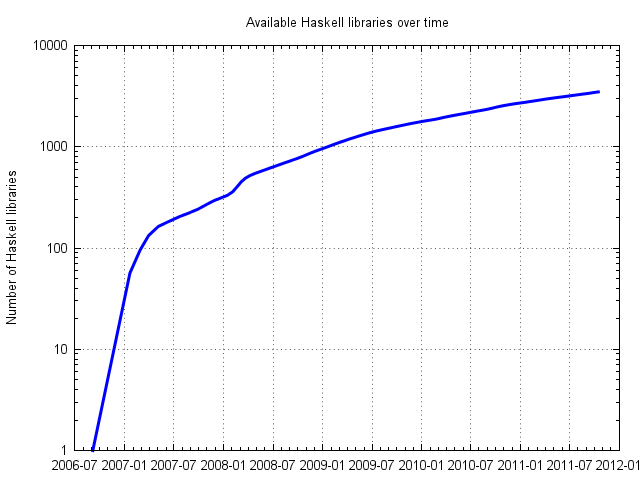
\includegraphics[width=12.5cm]{bilder/hackage.png}
\end{center}
\caption{The increasing data stock of hackageDB over the past five years}
\end{figure}

% currently just documentations accessible online

% \section{Motivation}

% doing a more complex project written in Hakell
% Hoogle, Hayoo as reference for Haskell functions
% Curr(y)gle > HayooI


% \section{Structure}

The further chapters of this theses are organized as follows. %
At first, \hyperref[preliminaries]{Chapter \ref*{preliminaries}} gives
the preliminiaries to understand this thesis. %
This includes basic information about the programming language Curry,
the representation of CurryDoc -- a tool to generate documentation of
a given Curry program,
and we introduce the Holumbus framework that is used to build the
search engine in connection with this thesis. %
In \hyperref[analysis]{Chapter \ref*{analysis}}, we analyze the
requirements to create an API search engine for Curry. %
It outlines the first ideas for the following implementation which is
given in \hyperref[implementation]{Chapter \ref*{implementation}}. %
Thereby, we focus on the most important implementation ideas and
decisions. %
At the very end, we discuss the results of this development. %
Also, we give a short outlook on features and ideas to expand the
given result. %
\chapter{Preliminaries}\label{preliminaries}
This chapter gives a brief introduction to background information that
are necessary to comprehend the following chapters. %
The first section gives an introduction to the programming language
Curry. %
It outlines main concepts and features of the language and gives short
explanations for a better understanding. %
The Curry implementation we refer to in the following sections is
PAKCS~\cite{pakcs}. Furthermore, we present CurryDoc~\cite{currydoc2}, a
tool to generate documentation that is distributed with PAKCS, in the
second section. %
The last section introduces the Holumbus\footnote{\url{http://holumbus.fh-wedel.de/trac}} framework, a
library written in Haskell to configure and build search engines. %

\section{The programming language Curry}\label{preliminaries:curry}

% Say that curry is a functional logic programming language and what
% this section is about.\\

Curry is a functional logic programming language that is an
international development project to provide a platform for research
and teaching mostly. %
As the description suggest, it offers features of both programming
paradigms. %
The first subsection will start with some general features, followed
by two subsections that cover functional and logic concepts of
Curry. %

% Start with the structure of a curry program. \\
\subsection{General Overview}
Like in Haskell, a program consists of function definitions and data
structures. %
A Curry module \emph{Test} is a program that is saved in a file named
\emph{Test.curry}. %
% After that explain how a function definition looks like and how
% pattern matching works (mention left-hand and right-hand
% side). Currys layout applies to the so called off-side rule. Add
% that Curry is strongly-typed and also type-inferred, so a signature
% is optional. \\
The syntax of a program is quite similar to Haskell, where function
application are also written in juxtaposition. %

\begin{hscode}\SaveRestoreHook
\column{B}{@{}>{\hspre}l<{\hspost}@{}}%
\column{E}{@{}>{\hspre}l<{\hspost}@{}}%
\>[B]{}\Varid{addTwo}\;\Varid{x}\mathrel{=}\Varid{x}\mathbin{+}\mathrm{2}{}\<[E]%
\ColumnHook
\end{hscode}\resethooks

The left-hand side of this function \ensuremath{\Varid{addTwo}\;\Varid{x}} is evaluated to the
right-hand side \ensuremath{\Varid{x}\mathbin{+}\mathrm{2}}, i.e., the call \ensuremath{\Varid{addTwo}\;\mathrm{3}} yields \ensuremath{\mathrm{3}\mathbin{+}\mathrm{3}\mathrel{=}\mathrm{5}}. %
Curry supports function definition with pattern matching, which is
often used in functional and logical programming languages. %
Pattern matching means that expressions with variables and data
constructors, like \ensuremath{\Conid{True}} and \ensuremath{\Conid{False}}, can occur in the arguments on
the left-hand side of a definition. %
The boolean operation \ensuremath{\neg }\footnote{Special characters are not
  allowed in Curry programs, we only use these symbols for the better
  understanding.} is a good example for a definition with pattern
matching. %
The definition distinguishes between more than one value, so we have
to write one rule for each possible input value. %

\begin{hscode}\SaveRestoreHook
\column{B}{@{}>{\hspre}l<{\hspost}@{}}%
\column{E}{@{}>{\hspre}l<{\hspost}@{}}%
\>[B]{}\neg \mathbin{::}\Conid{Bool}\to \Conid{Bool}{}\<[E]%
\\
\>[B]{}\neg \;\Conid{False}\mathrel{=}\Conid{True}{}\<[E]%
\\
\>[B]{}\neg \;\Conid{True}\mathrel{=}\Conid{False}{}\<[E]%
\ColumnHook
\end{hscode}\resethooks

The first line indicates that the function expects a boolean value as
argument and yields a boolean value as well\footnote{The symbol \ensuremath{\to }
  will be used for \emph{->} throughout this thesis}. %
The following two lines are rules, that describe that \ensuremath{\neg \;\Conid{False}}
yields \ensuremath{\Conid{True}}, whereas \ensuremath{\neg \;\Conid{True}} yields \ensuremath{\Conid{False}}. %
There are no more possible values for the argument of the function
\ensuremath{\neg }, since Curry is a strongly-typed language and \ensuremath{\Conid{True}} and \ensuremath{\Conid{False}}
are the only possible values with boolean type. %
In addition Curry also allows polymorphic functions. %
For instance, the identity function returns the argument that you
apply to the function, regardless of the input value's type. %
This means you can apply the function to all types of values, because
the type does not matter. %
You use a type variable in your type signature to indicate a
polymorphic type. %
The following code presents the type signature of the identity
function. %

\begin{hscode}\SaveRestoreHook
\column{B}{@{}>{\hspre}l<{\hspost}@{}}%
\column{E}{@{}>{\hspre}l<{\hspost}@{}}%
\>[B]{}\Varid{id}\mathbin{::}\Varid{a}\to \Varid{a}{}\<[E]%
\\
\>[B]{}\Varid{id}\;\Varid{value}\mathrel{=}\Varid{value}{}\<[E]%
\ColumnHook
\end{hscode}\resethooks

Overall a strong type system as well as polymorphism and pattern
matching are among Curry's general features. %
The next section covers functional characteristics of Curry.
% Mention that there are more concepts provided by Curry, which can be
% grouped by their underlying paradigm (use it as connection to the
% following subsections). Also the evaluation models are introduced.\\

% Curry is a functional logic programming language. As the name suggests
% it offers features of both programming paradigms. This section will
% outline the basic characteristics that Curry uses and give a short
% introduction to these characteristics.

% A program written in Curry is a collection of function definitions and
% data structures, which can be organized as a module. A module with the
% name \emph{M} is saved as \emph{M.curry} and can be imported in other
% modules. 
% The syntax of function definitions is quite similar to
% Haskell. Most functions are used as prefix operators, so the
% application of a function to an expression is denoted by
% juxtaposition. Arithmetic operators like |+| or |-| are infix
% operators like in the mathematical notation. Furthermore Curry also
% supports a conditional expression that corresponds to
% \emph{if-then-else}-expressions of other programming languages.

% In general one can say that Curry combines the features of the
% functional programming language Haskell and the logic programming
% language Prolog.

% \begin{itemize}
% \item pattern matching
% \item types (success)
% \item strongly typed
% \item type inference algorithm
% \item (pakcs) lazy, but incomplete - the strategy evaluates
%   non-deterministic choices sequentially instead of concurrently
% \item statically scoped (depends on layout - also: layout/off-side
%   rule), local scope with where and let
% \end{itemize}
\subsection{Functional Features}\label{preliminaries:curryInfo}
% Begin with data structures that als can be defined by the user. Use
% CurryInfo as example.\\
The boolean values mentioned in the previous section are part of the
predefined data types. %

\begin{hscode}\SaveRestoreHook
\column{B}{@{}>{\hspre}l<{\hspost}@{}}%
\column{E}{@{}>{\hspre}l<{\hspost}@{}}%
\>[B]{}\mathbf{data}\;\Conid{Bool}\mathrel{=}\Conid{True}\mid \Conid{False}{}\<[E]%
\ColumnHook
\end{hscode}\resethooks

This code defines a data type with the name \emph{Bool} that has
to constructors \ensuremath{\Conid{False}} and \ensuremath{\Conid{True}} with the type \ensuremath{\Conid{Bool}}. %
In this case the constructors are unary. %
Let's define a data structure that is more interesting and will be
used in the following chapters. %
For example a data structure that represents a Curry program, because
we want to create an API search engine for Curry. %
You can save a Curry program as a module and it exists of functions
and types (data structures). %

\begin{hscode}\SaveRestoreHook
\column{B}{@{}>{\hspre}l<{\hspost}@{}}%
\column{E}{@{}>{\hspre}l<{\hspost}@{}}%
\>[B]{}\mathbf{data}\;\Conid{CurryInfo}\mathrel{=}\Conid{CurryInfo}\;\Conid{ModuleInfo}\;[\mskip1.5mu \Conid{FunctionInfo}\mskip1.5mu]\;[\mskip1.5mu \Conid{TypeInfo}\mskip1.5mu]{}\<[E]%
\ColumnHook
\end{hscode}\resethooks

In this example \emph{CurryInfo} is the name of the type and also the
name of the constructor. %
As a constructor it needs three arguments, a \ensuremath{\Conid{ModuleInfo}} and a list
of \ensuremath{\Conid{FunctionInfo}} and \ensuremath{\Conid{TypeInfo}}. %
We define these data structures that hold the information about
specific proporties of the program in chapter 3. %

% Introduce the idea of higher-order functions.\\
Functions are first-class citizens in Curry. %
This means that they can appear as argument of an expression or even
in a data structure. %
The most popular use-case is the manipulation of all elements of a
list by a given function. %
PAKCS provides the function \ensuremath{\Varid{map}}, which also exists in Haskell, that
takes two arguments, a function and a list and returns a list. %
The important thing is that the type of the function matches the
elements of the list. %
For example, a function that converts an integer to a character can
be applied to a list of integers and yields to list of characters. %
The following code presents the a definition of the function \ensuremath{\Varid{map}}. %

\begin{hscode}\SaveRestoreHook
\column{B}{@{}>{\hspre}l<{\hspost}@{}}%
\column{E}{@{}>{\hspre}l<{\hspost}@{}}%
\>[B]{}\Varid{map}\mathbin{::}(\Varid{a}\to \Varid{b})\to [\mskip1.5mu \Varid{a}\mskip1.5mu]\to [\mskip1.5mu \Varid{b}\mskip1.5mu]{}\<[E]%
\\
\>[B]{}\Varid{map}\;\Varid{function}\;[\mskip1.5mu \mskip1.5mu]\mathrel{=}[\mskip1.5mu \mskip1.5mu]{}\<[E]%
\\
\>[B]{}\Varid{map}\;\Varid{function}\;(\Varid{element}\mathbin{:}\Varid{list})\mathrel{=}\Varid{function}\;\Varid{element}\mathbin{:}\Varid{map}\;\Varid{list}{}\<[E]%
\ColumnHook
\end{hscode}\resethooks

The syntax for lists is the same as in Haskell. %
\ensuremath{[\mskip1.5mu \mskip1.5mu]} is the empty list, whereas \ensuremath{\mathrm{1}\mathbin{:}\mathrm{2}\mathbin{:}\mathrm{3}\mathbin{:}[\mskip1.5mu \mskip1.5mu]} is the same as \ensuremath{[\mskip1.5mu \mathrm{1},\mathrm{2},\mathrm{3}\mskip1.5mu]} or
\ensuremath{\mathrm{1}\mathbin{:}[\mskip1.5mu \mathrm{2},\mathrm{3}\mskip1.5mu]}. %
The first representation is often used in pattern matching, to use the
first element of the list in the right-hand side of the definition. %
The first line presents the type signature. %
The function \ensuremath{(\Varid{a}\to \Varid{b})} takes a value of an unspecific type and returns
another unspecific type. %
The second argument is a list of elements with the type, that the
function expects. %
Furthermore, the resulting list contains elements that have the same
type as the resulting type of the function. %
The definition of map says that an empty list yields an empty list,
whereas the function is applied to the elements of a list with at
least one element recursively. %

% Explain lazy evaluation. Mention infinite structures.
The last functional concept Curry supports is \emph{lazy
  evaluation}. %
In general an expression is evaluated by replacing the left-hand side
of a definition by the right-hand side. %
The evaluation proceeds one replacement after another until it yields
a value. %
A value is an expression that does not consists of any defined
functions anymore, e.g. literals or data structures. %
If the last replacement does not result in a value, the evaluation
fails. %
If an evaluation has more than one possible replacement step, so
called subexpression can be evaluated. %
Lazy evaluation means that such a subexpression is only evaluated, if
its result is necessary to continue the evaluation and every
expression is evaluated just once. %

In summary Curry's functional programming features covers data
structures, higher-order functions and lazy evaluation as evaluation
strategy. %
Since the logic characteristics of Curry induce that there is another
strategy besides lazy evaluation, we will go one to the next section
and take a closer look into these characteristics. %
\subsection{Logic Features}
% Start with the connection between functional and logical programming:
% introduce the logical feature of non-deterministic functions. Therefor
% give an example for a rule and later a non-deterministic function.\\

Besides the already mentioned functional characteristics, Curry also
offers non-deterministic functions and logical variables. %
Logic programming languages consist of rules, for example a constant
function that represents my favourite number. %

\begin{hscode}\SaveRestoreHook
\column{B}{@{}>{\hspre}l<{\hspost}@{}}%
\column{E}{@{}>{\hspre}l<{\hspost}@{}}%
\>[B]{}\Varid{favouriteNumber}\;\Conid{Sandra}\mathrel{=}\mathrm{7}{}\<[E]%
\ColumnHook
\end{hscode}\resethooks

Let's now assume that I don't have one, but two favourite numbers. %
Curry as a hybrid of functional and logic programming language allows
multiple rules for function definitions. %

\begin{hscode}\SaveRestoreHook
\column{B}{@{}>{\hspre}l<{\hspost}@{}}%
\column{E}{@{}>{\hspre}l<{\hspost}@{}}%
\>[B]{}\Varid{favouriteNumber}\;\Conid{Sandra}\mathrel{=}\mathrm{3}{}\<[E]%
\\
\>[B]{}\Varid{favouriteNumber}\;\Conid{Sandra}\mathrel{=}\mathrm{7}{}\<[E]%
\ColumnHook
\end{hscode}\resethooks

This function is non-deterministic because it returns different values
for the same input. %
The pattern of this function overlaps in functional programming
languages, but Curry's ability to search for results allows to define
those non-deterministic functions. %

% After that explain how logical variables work.\\
% Give an example request with free variables. Mention the similarity
% to Prolog.
Curry also offers logical variables. %
A variable is called logical, if it appears on the right-hand side but
not on the left-hand side of a rule. %
These variables are unbound values, that are instantiated to evaluate
an expression. %
It is possible, that it exists more than one binding, since Curry
computes all possible solutions of an expression. %

% As connection to free variables, mention the evaluation methods
% ``narrowing'' and ``residuation'' next. Give an example with boolean and
% constraint equality. Connect this to flexible and rigid functions.\\

Curry provides two different approaches to evaluate an expression with
logical variables. %
The first approach suspends the evaluation in hopes that the logical
variable will be bound due to another evaluation of an expression. %
If there is no other expression to bind the value, the evaluation
fails. %
This approach is called residuation and Curry uses it for boolean
operators like the boolean equality \ensuremath{==}. %
The second approach, called narrowing, guesses a value for an unbound
value. %
Constraint operators like the boolean constraint \ensuremath{\mathbin{=.=}} use narrowing
for evaluation. %
In this context Curry distinguishes two types of operators: flexible
operators that narrow and rigid operators that use residuation. %
For example arithmetic (i.e. \ensuremath{\mathbin{+}}, \ensuremath{\mathbin{-}}, \ensuremath{\mathbin{*}} etc) and other primitive
operations are rigid. %
However these distinctions do not have any significance for
expressions without logical variables, so called \emph{ground
  expressions}. %
As mentioned in the previous section, Curry evaluates ground
expressions with lazy strategy.\\

Simply put, one can say that Curry combines the features of the
functional programming language Haskell and the logic programming
language Prolog. %

% \begin{itemize}
% \item Non-determinism
%   \begin{itemize}
%   \item choose
%   \item vs flexible functions
%   \item not in IO!
%   \end{itemize}
% \end{itemize}
\section{CurryDoc}\label{preliminaries:currydoc}
% Explain the idea of CurryDoc, mention the similarity to the known
% javadoc. Current status of the tool (HTML and LaTeX export).\\

CurryDoc is a tool to generate documentation for a program written in
Curry. %
The current version can generate either a HTML or \LaTeX~ file as
output. %
CurryDoc works similar to code generating tools like
javadoc\footnote{\url{http://www.oracle.com/technetwork/java/javase/documentation/index-jsp-135444.html}}
as it uses the comments in the source code, which are provided by the
user, to gain information about the function or data structure. %
It also provides the type signatures of functions, since Curry uses a
type inferencer algorithm. %
In addition the CurryDoc tool analyzes the program's structure and
approximates the run-time behavior to gain further
information~\cite{currydoc2}. %
This analysis includes information about in-/completeness, overlapping
pattern matches and non-/deterministic functions. %

Since CurryDoc is implemented in Curry, it uses the meta-programming
module
\emph{FlatCurry}\footnote{\url{http://www.informatik.uni-kiel.de/~pakcs/lib/CDOC/FlatCurry.html}}
that provides an intermediate language of the Curry program to analyze
the special function proporties. %
Such a FlatCurry~\cite{flat} program consists mainly of a list of
functions, a list of types and information about the module itself. %
% As you may notice, these are the informations we want to provide for
% the API search engine.

% Introduce FlatCurry program as utility. What is FlatCurry? Give an example of a
% Curry program and the corresponding FlatCurry program.\\

\section{The Holumbus Framework}\label{preliminaries:holumbus}
The Holumbus Framework is a Haskell library created by students of FH
Wedel in connection with three master's theses~\cite{searchingthesis}\cite{indexingthesis}. %
Holumbus is a library to build and configure a search engine. %
The main idea of the framework is to collect data with a specific
structure, like an API of a programming language, and to take
advantage of this structure to improve the search results. %
In addition to the framework, they also build an example application
named \emph{Hayoo!}~\cite{hayoo}, an API search engine for the
functional programming language Haskell. %

The framework supports three steps to create a search engine: the
crawling (1), the indexing (2) and the searching part (3) itself. %
\begin{enumerate} 
\item In the process of crawling, the World Wide Web is browsed
  automatically in order to collect all data and information
  respectively. %  
  Crawlers mainly copy all the visited pages, which then, are passed
  to the indexer in order to preprocess the data. %
\item The indexing describes a process to analyze and store data in
  order to provide a fast information retrieval. %
  The indexer preprocess the data in order to filter all relevant
  search criteria, e.g., an indexer can filter nothing and store each
  word of the given data. %
  Additionally, instead of keeping a copy of the original document,
  e.g., a web page, a characteristically data structure
  is created. %
\item Eventually, this fast information retrieval is the heart of the
  search engine. %
  One can access the information of the index by phrasing a search
  query. %
  Commonly, the search query is compared to the information stored in
  the index and convenient matches, i.e., documents, are returned as
  results. %
\end{enumerate}
We focus on the latter two steps, since we use them in our
implementation. %
Holumbus provides several modules for the indexing process (see
\hyperref[fig:holumbus]{Figure \ref*{fig:holumbus}}). %
Common provides interfaces for the data structure; This data structure
is composed of two parts: the index and documents. %
Holumbus calls the structure to hold the preprocessed data
\emph{index} and \emph{documents} is the name for new created data
structure. %
Further data structures that are used in the indexing process are
stores in the folder \emph{Common}, whereas \emph{Inverted} consists
of the implementation of the actual indexed data. %
In this case, Holumbus decided on a structure called \emph{inverted
  filed} or \emph{inverted index}. %
This structure stores the occurrences of each search criterion and a
reference to its corresponding document. %
Furthermore, Holumbus provides the mechanism to form a search request,
to process this request and a data structure to represent the result;
additionally, this result can be subjected to a ranking. %
(see \hyperref[fig:holumbus]{Figure \ref*{fig:holumbus}} again). %

\tikzstyle{every node}=[draw=black,thick,anchor=west]
\tikzstyle{selected}=[draw=red,fill=red!30]
\tikzstyle{optional}=[dashed]
\tikzstyle{file}=[rounded corners=2mm]
\begin{figure}[h!]
\begin{center}
\begin{tikzpicture}[%
  grow via three points={one child at (0.5,-0.7) and
  two children at (0.5,-0.7) and (0.5,-1.4)},
  edge from parent path={(\tikzparentnode.south) |- (\tikzchildnode.west)}]
  \node {Holumbus}
    child { node [optional] {Crawler} }		
    child { node [optional] {Data} }
    child { node {Index} }
    child { node {Query} };
\end{tikzpicture}
\begin{tikzpicture}[%
  grow via three points={one child at (0.5,-0.7) and
  two children at (0.5,-0.7) and (0.5,-1.4)},
  edge from parent path={(\tikzparentnode.south) |- (\tikzchildnode.west)}]
  \node {Query}
    child { node [optional] {Language} 
      child {node [file] {Grammar}}
      child {node [file,optional] {Parser}}}	
    child [missing] {}
    child [missing] {}
    child { node [file] {Processor} }
    child { node [file] {Ranking} }
    child { node [file] {Result} };
\end{tikzpicture}
\begin{tikzpicture}[%
  grow via three points={one child at (0.5,-0.7) and
  two children at (0.5,-0.7) and (0.5,-1.4)},
  edge from parent path={(\tikzparentnode.south) |- (\tikzchildnode.west)}]
  \node {Index}
    child { node {Common}}
    child { node [file] {Common}}
    child { node [file] {CompactDocuments} }
    child { node [file] {CompactIndex} }
    child { node {Inverted} };
\end{tikzpicture}
\end{center}
\caption{Directory Structure of the Holumbus Library}
\label{fig:holumbus}
\end{figure}
\chapter{Analysis}\label{analysis}
This chapter looks into the requirements to build and run Curr(y)gle,
an API search engine for Curry. %
The first section deals with the creation of an index, whereas the
second and third section addresses the process of searching for a
query. %
In this context, we take a closer look of the Holumbus framework and
its features related to searching and evaluate the criteria to
accomplish a user-friendly search mechanism. %
Furthermore, we discuss the features Curr(y)gle should provide to
specify a search query. %

% Above all we need a web application to handle user queries, which is
% analyzed in the last section.

% Give a short summary about the following sections.\\

% What do we need to create this search engine? 
% The possibility to generate and update the index.\\
% The possibility to search for these informations in the index. At
% best: user-friendly \\

% What do we want above all?
% A web application for queries.

% \section{Currydoc}

\section{Creating the Index}\label{analysis:indexer}
Search engines look up information, hence, we need to collect data
that we can search for. %
This data is called index and stores all the information we want to
provide. %
In our case, we want to collect data that relates to the API of
Curry. %
Therefore, we need to think what kind of information we can provide
and decide what we want to search for. %
Secondly, we introduce the data structure provided by the Holumbus
framework that holds these information.\\ %


% The data we want to extract from a given Curry module includes at
% least the list of defined functions and data types. %
% We also want to consider the name, corresponding module and
% description of these functions and data types. %
% Additionally, general information about the module like its name and
% author needs to be stored. %

Usually, a web crawler is applied to browse the world wide web for
data. %
But since Curry is currently organized by the module documentation
generated by CurryDoc, we already have a mechanism to gain these
information about a Curry module. %
In fact, we even have more function-related information % we stated
% in the \hyperref[preliminaries:curryInfo]{previous chapter} 
because we know if a function definition is non-deterministic or
deterministic and if a given function is flexible or rigid. %
In the following, we refer to these characteristics as contexts and the
following listing presents the information or, more precisely, the
contexts that we want to provide: %

\begin{itemize}
\item name (for modules, functions and types)
\item description (for modules, function and types)
\item type signatures (for functions and types)
\item corresponding module (for functions and types)
\item author (module)
\item rigid and flexible characteristics (function)
\item non-/deterministic characteristics (function)
\end{itemize}

CurryDoc processes Curry modules and generates documentation as HTML
or \LaTeX{} output. %
For our index, we are not interested in any document markup language,
but the pure information about the Curry module. %
This observation leads to the idea of generating a new readable data
structure as an extension to CurryDoc. %
In the process we take advantage of the FlatCurry representation of a
Curry module to access these information we mentioned above. %
We discuss the actual implementation in
\hyperref[implementation:currydoc]{Section
  \ref{implementation:currydoc}}. %
In preparation of the next chapter, we introduce the data
structure \ensuremath{\Conid{TypeExpr}} that is provided by the FlatCurry module. %

\begin{hscode}\SaveRestoreHook
\column{B}{@{}>{\hspre}l<{\hspost}@{}}%
\column{4}{@{}>{\hspre}l<{\hspost}@{}}%
\column{6}{@{}>{\hspre}l<{\hspost}@{}}%
\column{E}{@{}>{\hspre}l<{\hspost}@{}}%
\>[B]{}\mathbf{data}\;\Conid{TypeExpr}\mathrel{=}{}\<[E]%
\\
\>[B]{}\hsindent{6}{}\<[6]%
\>[6]{}\Conid{TVar}\;\Conid{TVarIndex}{}\<[E]%
\\
\>[B]{}\hsindent{4}{}\<[4]%
\>[4]{}\mid \Conid{FuncType}\;\Conid{TypeExpr}\;\Conid{TypeExpr}{}\<[E]%
\\
\>[B]{}\hsindent{4}{}\<[4]%
\>[4]{}\mid \Conid{TCons}\;\Conid{QName}\;[\mskip1.5mu \Conid{TypeExpr}\mskip1.5mu]{}\<[E]%
\ColumnHook
\end{hscode}\resethooks


\ensuremath{\Conid{TypeExpr}} represents type expression used in function and data type
signatures. %
It consists of three constructors to distinguish between %
\begin{itemize}
\item a function type - \ensuremath{\Conid{FuncType}\;\Conid{TypeExpr}\;\Conid{TypeExpr}} 
\item a type variable  - \ensuremath{\Conid{TVar}\;\Conid{TVarIndex}} and 
\item a type constructor application - \ensuremath{\Conid{TCons}\;\Conid{QName}\;[\mskip1.5mu \Conid{TypeExpr}\mskip1.5mu]}
\end{itemize}

For the latter, the list of \ensuremath{\Conid{TypeExpr}} stand for the type arguments. %
Furthermore, \ensuremath{\Conid{TVarIndex}} is just a type synonym for \ensuremath{\Conid{Int}} and \ensuremath{\Conid{QName}}
represents a qualified name consisting of the module's name and the
function's or type constructor's name. %
\ensuremath{\Conid{QName}} is a type synonym for a tuple \ensuremath{(\Conid{String},\Conid{String})}. %
An unary type like \ensuremath{\Conid{Bool}} is represented as a type constructor with an
empty list, i.e. without an application to type arguments. %
The following code shows some signatures and their representation in
the \ensuremath{\Conid{TypeExpr}} data structure. %

\begin{figure}[h!]
\begin{hscode}\SaveRestoreHook
\column{B}{@{}>{\hspre}l<{\hspost}@{}}%
\column{3}{@{}>{\hspre}l<{\hspost}@{}}%
\column{E}{@{}>{\hspre}l<{\hspost}@{}}%
\>[B]{}\Conid{TCons}\;(\Conid{Prelude},\Conid{Maybe})\;{}\<[E]%
\\
\>[B]{}\hsindent{3}{}\<[3]%
\>[3]{}[\mskip1.5mu (\Conid{TCons}\;(\Conid{Prelude},\Conid{Int})\;[\mskip1.5mu \mskip1.5mu]),{}\<[E]%
\\
\>[B]{}\hsindent{3}{}\<[3]%
\>[3]{}(\Conid{TCons}\;(\Conid{Prelude},[\mskip1.5mu \mskip1.5mu])\;[\mskip1.5mu (\Conid{TCons}\;(\Conid{Prelude},\Conid{Char}))\mskip1.5mu])\mskip1.5mu]{}\<[E]%
\ColumnHook
\end{hscode}\resethooks
\caption{The representation of \ensuremath{\Conid{Maybe}\;\Conid{Int}\;\Conid{String}} as \ensuremath{\Conid{TypeExpr}}}
\end{figure}
\begin{figure}[h!]
\begin{hscode}\SaveRestoreHook
\column{B}{@{}>{\hspre}l<{\hspost}@{}}%
\column{E}{@{}>{\hspre}l<{\hspost}@{}}%
\>[B]{}\Conid{FuncType}\;(\Conid{TCons}\;(\Conid{Prelude},\Conid{IO})\;[\mskip1.5mu \Conid{TVar}\;\mathrm{97}\mskip1.5mu])\;(\Conid{TCons}\;(\Conid{Prelude},\Conid{IO})\;[\mskip1.5mu \Conid{TVar}\;\mathrm{97}\mskip1.5mu]){}\<[E]%
\ColumnHook
\end{hscode}\resethooks
\caption{The representation of \ensuremath{\Conid{IO}\;\Varid{a}\to \Conid{IO}\;\Varid{a}} as \ensuremath{\Conid{TypeExpr}}}
\end{figure}
\begin{figure}[h!]
\begin{hscode}\SaveRestoreHook
\column{B}{@{}>{\hspre}l<{\hspost}@{}}%
\column{E}{@{}>{\hspre}l<{\hspost}@{}}%
\>[B]{}\Conid{FuncType}\;(\Conid{TCons}\;(\Conid{Prelude},\Conid{Bool})\;[\mskip1.5mu \mskip1.5mu])\;{}\<[E]%
\\
\>[B]{}(\Conid{FuncType}\;(\Conid{TCons}\;(\Conid{Prelude},\Conid{Int})\;[\mskip1.5mu \mskip1.5mu]))\;(\Conid{TCons}\;(\Conid{Prelude},\Conid{Int})\;[\mskip1.5mu \mskip1.5mu])){}\<[E]%
\ColumnHook
\end{hscode}\resethooks
\caption{The representation of \ensuremath{\Conid{Bool}\to \Conid{Int}\to \Conid{Int}} as \ensuremath{\Conid{TypeExpr}}}
\end{figure}

% What do we need to create an index that can be used for the Curry
% search engine?\\

% First: Curry specific information (CurryDoc)\\

% First start with the idea of the extension: instead of generating a
% document markup language, generate a readable data structure.\\

% Introduce the TypeExpr data structure that is part of the FlatCurry
% feature.\\

% Second: a data structure to hold the information (index and document
% structure from the Holumbus framework)\\

After we decide about the contents of the index, we need to discuss
the storage of these information. %
We make use of the Holumbus framework that provides data structures to
manage the collected data and interfaces to operate on these
structures. %a
The main idea is to use two structures to store the data, one for the
documents we are indexing and the other one stores the actual data we
traverse when a search is performed. %

At first, we introduce the data structures we use in our
implementation, which are provided by the framework. %
Secondly, we discuss the functionality of the interfaces. \\

In our implementation, we use \ensuremath{\Conid{Documents}\;\Varid{a}} as a data structures to
store the documents we are indexing, where \ensuremath{\Varid{a}} is the type of the
document. %
Each document of a collection has its unique identifier. %
For example, we want to construct the index for the Curry modules
\ensuremath{\Conid{Prelude}}, \ensuremath{\Conid{IO}} and \ensuremath{\Conid{Maybe}} and modules are represented
by a data structure \ensuremath{\Conid{ModuleInfo}}. %
Then these modules are the stored in \ensuremath{\Conid{Documents}\;\Conid{ModuleInfo}}. %
In order to simplify the idea, we sketch the example in pseudocode,
where the names of the modules represent values of the \ensuremath{\Conid{ModuleInfo}}
data structure. %

{\small
\begin{hscode}\SaveRestoreHook
\column{B}{@{}>{\hspre}l<{\hspost}@{}}%
\column{E}{@{}>{\hspre}l<{\hspost}@{}}%
\>[B]{}\{\mskip1.5mu (\Conid{Prelude},\mathrm{1}),(\Conid{IO},\mathrm{2}),(\Conid{Maybe},\mathrm{3})\mskip1.5mu\}{}\<[E]%
\ColumnHook
\end{hscode}\resethooks
}
Thus, \ensuremath{\Conid{Documents}\;\Varid{a}} can be described as a collection of documents,
where each document can be determined unambiguously.

Secondly the framework provides a structure \ensuremath{\Conid{Inverted}} for the actual
index data structure that is traversed in the search process. %
Simply put, the index stores pairs strings, where the
second entry is the word that can be searched and the first entry is
the context of this word. %
In order to provide another example, let's assume we have a Curry
module \ensuremath{\Conid{Duck}} and the following information about this module:

{\small
\begin{hscode}\SaveRestoreHook
\column{B}{@{}>{\hspre}c<{\hspost}@{}}%
\column{BE}{@{}l@{}}%
\column{4}{@{}>{\hspre}l<{\hspost}@{}}%
\column{E}{@{}>{\hspre}l<{\hspost}@{}}%
\>[B]{}({}\<[BE]%
\>[4]{}\text{\tt \char34 name\char34},\text{\tt \char34 Duck\char34}){}\<[E]%
\\
\>[B]{}({}\<[BE]%
\>[4]{}\text{\tt \char34 author\char34},\text{\tt \char34 Donald\char34}){}\<[E]%
\\
\>[B]{}({}\<[BE]%
\>[4]{}\text{\tt \char34 description\char34},{}\<[E]%
\\
\>[4]{}\text{\tt \char34 If~it~quacks~like~a~duck~\&~walks~like~a~duck,~it's~a~duck.\char34}){}\<[E]%
\ColumnHook
\end{hscode}\resethooks
}
% An example for our API search engine is the pair |(\textss{author},
% \textss{Donald Duck})|, with a context \emph{author},
% whose corresponding string is the author of a Curry
% module. %
As addition to the design, the identifier of the document is stored in
the index data structure to provide an association between the index
and the document the data was indexed from. %

In fact, this concept is called \emph{inverted index} or
\emph{inverted file}, which explains the name of the data type. %
Thus, in the end, the index is a collection of triples. %

{\small
\begin{hscode}\SaveRestoreHook
\column{B}{@{}>{\hspre}l<{\hspost}@{}}%
\column{3}{@{}>{\hspre}l<{\hspost}@{}}%
\column{6}{@{}>{\hspre}l<{\hspost}@{}}%
\column{E}{@{}>{\hspre}l<{\hspost}@{}}%
\>[B]{}\Conid{Documents}\mathrel{=}\{\mskip1.5mu (\Conid{Prelude},\mathrm{1}),(\Conid{IO},\mathrm{2}),(\Conid{Maybe},\mathrm{3}),(\Conid{Duck},\mathrm{4})\mskip1.5mu\}{}\<[E]%
\\
\>[B]{}\Conid{Inverted}\mathrel{=}{}\<[E]%
\\
\>[B]{}\hsindent{3}{}\<[3]%
\>[3]{}({}\<[6]%
\>[6]{}\text{\tt \char34 name\char34},\text{\tt \char34 Duck\char34},\mathrm{4}){}\<[E]%
\\
\>[B]{}\hsindent{3}{}\<[3]%
\>[3]{}(\text{\tt \char34 author\char34},\text{\tt \char34 Donald\char34},\mathrm{4}){}\<[E]%
\\
\>[B]{}\hsindent{3}{}\<[3]%
\>[3]{}(\text{\tt \char34 description\char34},\text{\tt \char34 If~it~quacks~[...]~it's~a~duck.\char34},\mathrm{4}){}\<[E]%
\ColumnHook
\end{hscode}\resethooks
}

Another type provided by the framework is \ensuremath{\Conid{HolumbusState}\;\Varid{a}}: a
combination of index and documents, polymorph by the data the documents
hold. %
For the examples presented above, we would use \ensuremath{\Conid{HolumbusState}\;\Conid{ModuleInfo}} for the index. %
In \hyperref[implementation:index]{Section \ref{implementation:index}}
we illustrate the use of these data structures in our implementation.

Holumbus provides more than these two explicit data structures to
handle the storage, it rather has multiple implementations to choose
from. %
All these implementations of the documents and index data structure
are instances of the provided interfaces. %
Therefore, we introduce the main functionalities of the interfaces we
use in our implementation. %
\ensuremath{\Conid{HolIndex}} is the name of the interface for the indexed data and the
main functionalities we are interested in, are the provided methods to
create a new triple and merge two existing structures. %
We need the same functionality for \ensuremath{\Conid{HolDocuments}}, the interface for
the document collection. %
Besides methods to merge two document collections and create a new one,
a function to change the identifier of each document in the collection
and to insert a document is provided as well.\\

To sum up, we want to extend the current CurryDoc implementation to
generate a new readable data structure about a given Curry module. %
These information cover, among other things, function and data
structure definitions, user comments and description in the source
code, and general information about the module. %
This new data structure determines the type of \ensuremath{\Conid{HolDocuments}\;\Varid{a}} and
forms one part of the index-document-duo that Holumbus provides. %

% \begin{itemize}
% \item HolDocuments - Stores the documents that correspond to the
%   index. A mapping is provided.
% \item HolIndex - Data structure to store the information, that is
%   traversed in the search process.
% \item HolumbusState a - the combination of index and document,
%   polymorph by the data the HolDocuments holds.
% \end{itemize}

\section{Searching}
% How do we search for the information in the index?
After creating the skeleton for the index and its storage, we want to
actually use these information in a search query. %
Thus, the first step is to think about the structure of a query, in the
second step we process the query and last we need a representation of
the results of the processed query for further use.\\

Fortunately, these are all features the Holumbus framework provides. At
first, we take a look at the search mechanism and the query representation. %
The data structure \ensuremath{\Conid{Query}} allows to search for a word and a phrase,
both case-insensitive and case-sensitive. %

\begin{hscode}\SaveRestoreHook
\column{B}{@{}>{\hspre}l<{\hspost}@{}}%
\column{3}{@{}>{\hspre}l<{\hspost}@{}}%
\column{E}{@{}>{\hspre}l<{\hspost}@{}}%
\>[B]{}\mathbf{data}\;\Conid{Query}\mathrel{=}{}\<[E]%
\\
\>[B]{}\hsindent{3}{}\<[3]%
\>[3]{}\Conid{Word}\;\Conid{String}\mid {}\<[E]%
\\
\>[B]{}\hsindent{3}{}\<[3]%
\>[3]{}\Conid{Phrase}\;\Conid{String}\mid {}\<[E]%
\\
\>[B]{}\hsindent{3}{}\<[3]%
\>[3]{}\Conid{CaseWord}\;\Conid{String}\mid {}\<[E]%
\\
\>[B]{}\hsindent{3}{}\<[3]%
\>[3]{}\Conid{CasePhrase}\;\Conid{String}\mid {}\<[E]%
\\
\>[B]{}\hsindent{3}{}\<[3]%
\>[3]{}\mathbin{...}{}\<[E]%
\ColumnHook
\end{hscode}\resethooks

Since the search depends on user-input, the framework also allows
\emph{fuzzy searching} to scan for results with spelling errors like
transposed letters. %
Since the index data structure of Holumbus uses pairs of words and
contexts, a special mechanism to search for one or more contexts is
given. %
Furthermore, the structure provides binary operators to combine
multiple queries; supported operators are conjunctions, disjunctions and
negations. %

\begin{hscode}\SaveRestoreHook
\column{B}{@{}>{\hspre}l<{\hspost}@{}}%
\column{3}{@{}>{\hspre}l<{\hspost}@{}}%
\column{E}{@{}>{\hspre}l<{\hspost}@{}}%
\>[B]{}\mathbf{data}\;\Conid{Query}\mathrel{=}{}\<[E]%
\\
\>[B]{}\hsindent{3}{}\<[3]%
\>[3]{}\mathbin{...}\mid {}\<[E]%
\\
\>[B]{}\hsindent{3}{}\<[3]%
\>[3]{}\Conid{FuzzySearch}\;\Conid{String}\mid {}\<[E]%
\\
\>[B]{}\hsindent{3}{}\<[3]%
\>[3]{}\Conid{Specifier}\;[\mskip1.5mu \Conid{Context}\mskip1.5mu]\;\Conid{Query}\mid {}\<[E]%
\\
\>[B]{}\hsindent{3}{}\<[3]%
\>[3]{}\Conid{BinQuery}\;\Conid{BinOp}\;\Conid{Query}\;\Conid{Query}{}\<[E]%
\\[\blanklineskip]%
\>[B]{}\mathbf{type}\;\Conid{Context}\mathrel{=}\Conid{String}{}\<[E]%
\\
\>[B]{}\mathbf{data}\;\Conid{BinOp}\mathrel{=}\Conid{And}\mid \Conid{Or}\mid \Conid{But}{}\<[E]%
\ColumnHook
\end{hscode}\resethooks

% And this data structure can be processed by processQuery (Holumbus.Query.Processor).
As next step, we pass the index, document and query to the function
\emph{processQuery} that, as the name suggests, processes the query. %
When processing the query, Holumbus only matches for prefixes of the
given word or phrase in a query, we need to keep this restriction in mind
when we create the index in \hyperref[implementation:index]{Section
  \ref{implementation:index}}. %


The return value of the successfully processed query is a data
structure \ensuremath{\Conid{Result}\;\Varid{a}} that consists of the matching documents with type
\ensuremath{\Varid{a}} as well as possible word completions. %

\begin{hscode}\SaveRestoreHook
\column{B}{@{}>{\hspre}l<{\hspost}@{}}%
\column{3}{@{}>{\hspre}l<{\hspost}@{}}%
\column{16}{@{}>{\hspre}l<{\hspost}@{}}%
\column{23}{@{}>{\hspre}l<{\hspost}@{}}%
\column{E}{@{}>{\hspre}l<{\hspost}@{}}%
\>[B]{}\mbox{\onelinecomment  Pseudocode with Haskell syntax}{}\<[E]%
\\
\>[B]{}\mathbf{data}\;\Conid{Result}\;\Varid{a}{}\<[16]%
\>[16]{}\mathrel{=}\Conid{Result}{}\<[E]%
\\
\>[B]{}\hsindent{3}{}\<[3]%
\>[3]{}\{\mskip1.5mu \Varid{documents}{}\<[23]%
\>[23]{}\mathbin{::}(\Conid{Document}\;\Varid{a},\Conid{Score}){}\<[E]%
\\
\>[B]{}\hsindent{3}{}\<[3]%
\>[3]{},\Varid{word}\;\Varid{completions}{}\<[23]%
\>[23]{}\mathbin{::}(\Conid{String},\Conid{Score}){}\<[E]%
\\
\>[B]{}\hsindent{3}{}\<[3]%
\>[3]{}\mskip1.5mu\}{}\<[E]%
\\
\>[B]{}\mathbf{type}\;\Conid{Score}\mathrel{=}\Conid{Float}{}\<[E]%
\ColumnHook
\end{hscode}\resethooks

Additionally, each document and word completion has a calculated score between \ensuremath{\mathrm{0}} and \ensuremath{\mathrm{1}} that determines the
relevance of the result. %
For documents, this score is calculated by the number of occurrences of
the search query in the document by default and represented as float. %
But Holumbus also provides a mechanism to apply a customized ranking
function to calculate the score. %

If we proceed the examples of the last section, we can construct the
query

\begin{hscode}\SaveRestoreHook
\column{B}{@{}>{\hspre}l<{\hspost}@{}}%
\column{E}{@{}>{\hspre}l<{\hspost}@{}}%
\>[B]{}\Conid{Specifier}\;[\mskip1.5mu \text{\tt \char34 description\char34}\mskip1.5mu]\;\text{\tt \char34 quack\char34}{}\<[E]%
\ColumnHook
\end{hscode}\resethooks

and after processing, we get all modules, i.e. documents, which
description consists of the word \textss{quack} and all possible word
completions (the scores a random values to complete the example). %

\begin{hscode}\SaveRestoreHook
\column{B}{@{}>{\hspre}l<{\hspost}@{}}%
\column{11}{@{}>{\hspre}l<{\hspost}@{}}%
\column{E}{@{}>{\hspre}l<{\hspost}@{}}%
\>[B]{}\Conid{Result}\mathrel{=}{}\<[11]%
\>[11]{}\{\mskip1.5mu \Varid{documents}\mathbin{:}\{\mskip1.5mu (\text{\tt \char34 Duck\char34},\mathrm{1}),\mathrm{0.75}\mskip1.5mu\}\mskip1.5mu\},{}\<[E]%
\\
\>[11]{}\{\mskip1.5mu \Varid{word}\;\Varid{completions}\mathbin{:}\{\mskip1.5mu \text{\tt \char34 quacks\char34},\mathrm{0.8}\mskip1.5mu\}\mskip1.5mu\}{}\<[E]%
\ColumnHook
\end{hscode}\resethooks

% The first is represented by |DocHits a| that is a mapping of |DocInfo
% a|, the contexts and the document's unique identifier. %
% On the other hand |DocInfo a| consists of the matching document and a
% score. %

% \begin{code} 
% data DocInfo a = DocInfo 
%   { document :: (Document a)
%   , docScore  :: Score
%  }
% type DocContextHits    = Map Context DocWordHits

% type DocWordHits       = Map Word Positions

% type DocHits a  = DocIdMap (DocInfo a, DocContextHits)
% \end{code}

% By default this score is calculated by the number of occurrences of
% the search query in the document and represented as |Float|. %
% But Holumbus also provides a mechanism to apply a customized ranking
% function to calculate the score. %
% |WordHits| illustrates the word completions and is represented by a
% mapping of the possible completions of the given prefix in combination
% with its score, i.e. |WordInfo|, and the contexts.\\
% Holumbus also provides a data structure that is returned after a query

% \begin{code}
% data WordInfo  = WordInfo 
%                 { terms     :: Terms
%                 , wordScore :: Score                
%                 }

% type WordHits          = Map Word (WordInfo, WordContextHits)

% type WordContextHits   = Map Context WordDocHits

% type WordDocHits       = Occurrences
% \end{code}


Summing up, we have discussed the mechanism to evaluate a query with
the Holumbus framework. %
The provided mechanism includes the data structures to represent a
query, which can be processed to a data structure consisting of the
matching documents and possible word completions. %
% But first the user input has to be parsed into the query structure to
% start the processing.

\section{Parsing User-Queries}\label{analysis:parser}
% Which criteria do we want to search for? Modules, functions, types,
% signatures, and  det./non-det., flexible/rigid functions. \\
The next question is how to construct the query for a given
user-input. %
At first we have to decide about the criteria users can search for. %
Since the index provides the pairs of contexts and search words, we
are able to restrict the search to all these contexts with the help of
the \ensuremath{\Conid{Query}} data structure and the \ensuremath{\Conid{Specifier}} constructor. %
This structure of the index allows us to search for modules,
functions, types, signatures and all other contexts we use during the
creation of the index.\\

% First describe the idea, that the use of a specific language increases
% the usability. But it also restricts the user in her usage of the
% search engine, if this language gets more complex. So this results in
% a compromise between a simply to use language and a language that can
% be parsed.  Show the example of searching IO, where the restriction to
% modules minimizes the result.\\
The search mechanism as part of the user-experience is supposed to be
as simple as possible. %
The right use of a specific language can increase the usability. %
A good example is the search term \ensuremath{\text{\tt \char34 io\char34}}, since in Curry \emph{IO}
is the name for a module, a type and a constructor. %
Furthermore, there are many functions in the IO module that contain
the word \emph{io}. Thus, the search for \emph{io} results in a great
amount of hits. %
We can restrict the search to a specific context to reduce the number
of hits. %
Therefore, we want to provide specifiers the user combines with the
search term, for example \ensuremath{\text{\tt \char34 :function~IO\char34}} searches for \emph{IO} in
the context of function names only. %
But this special syntax restricts the user in the use of the search
engine, if the language gets more complex. %
Thus, in order to provide a user-friendly search engine, we have to make a
compromise between a simple language and a language that can be
parsed. %

% Set the focus on signatures. Because Hayoo! does not find signatures with
% redundant parentheses, Curr(y)gle supports parenthesized signatures
% and parenthesized query parts in general. \\
Besides these specifiers we want to parse type signatures of Curry
functions and data types. %
During our test phase, we also studied Hayoo!, the first search engine
that was build with the Holumbus Framework. %
We recognized that Hayoo! is not able to parse redundant parenthesized
signatures.  In our opinion, this parsing behavior can be irritating
in the usage of the search engine, therefore, we want to address the
problem of redundant parentheses with great care when we parse
signatures. %
For instance, let's assume a beginner searches for a function with the
type signature \ensuremath{\text{\tt \char34 IO~->~(IO~Int)\char34}}. %
The type \emph{IO Int} and type constructors in general do not need
parentheses, but as beginner you might think they do. %
Thus, we want to support parenthesized signatures and parenthesized
query parts in general. %

Last but not least we want to provide binary conjunctions like
\emph{And}, \emph{Or} and \emph{Not}. %
On the one hand, a combination of more search words is desirable
because popular search engines like Google\texttrademark~ support
binary operations as feature. %
The popularity increases the probability that users assume binary
operations are standard features and expect search engines to provide
the conjunction of several search terms. %
On the other hand, if the desired result is still vague, a combination
of more search words by a disjunction \emph{Or} helps to narrow down
the search results.\\
% In addition: binary operations/conjunctions. \\
% Explain that in most cases, a combination of more search words is
% desirable, because first popular search engines like Google\texttrademark~use this
% feature so it's common knowledge (the user expects this features) and
% second it's easier to search for more search words, if the desired
% result is still vague.

In the end, we want to provide an intuitive but powerful syntax for
the search engine. %
With specifiers to restrict the search results to a given context and
with binary operations to narrow down or extend the contexts, we want
to provide a simple language for the user queries. %
Additionally, type signatures should be recognized, including
function, construction and primitive types as well as redundant
parenthesized signatures. %
As the number of the supported features increases, the query gets more
complex to read. %
Thus, to reach this goal, we need to analyse the user input and
rebuild it as an expression of our \ensuremath{\Conid{Query}} data structure. %
The following figures describe the language the parser supports and in
\hyperref[implementation:parser]{Section \ref{implementation:parser}}
we discuss our actual implementation. % 

\chapter{Implementation}\label{implementation}
% Mention that the implementation is done in Haskell or Curry.\\
% Give a short summary of the next sections.

This chapter presents the implementation of the search engine on the
basis of some code examples and the corresponding design ideas and
decisions. %
After we give a short overview of the Curry and Haskell project in
general, we take a look at the extension for the current version of
CurryDoc. %
In this context we illustrate the interaction between this extension
and the index creation. %
The latter determines the topic of the second section. %
We specify the index and document data in more detail and state some
difficulties that arose due to the usage of the Holumbus framework. %
The third section addresses the implemented parser to convert the user
input into a query that can be processed by Holumbus. %
We illustrate the general idea and implementation approach of a parser
to introduce into the subject. %
Furthermore, we give an excerpt of the implemented parser. %

The last step to our search engine is the application itself. %
In order run the search engine as web application, we use the
\emph{Snap
  Framework}\footnote{\url{http://snapframework.com/about}}. %
Snap is a Haskell library to simplify web development on unix
systems. % 
We do not go into detail on this topic, albeit, the simple usage to
run the application is shown in \hyperref[currysearch]{Appendix
  \ref{currysearch}}. %
% The last section covers features and implementations of the web
% application for the search engine. %

\section{Environment}

The underlying environment for the development is an Apple 64-bit Mac OS
X/Version 10.7.4 system. %
Further, the implementations are mostly written in the functional
programming language Haskell; we use the functional logic programming
language
Curry for the CurryDoc extension only.\\
For the Haskell implementation, we use the Glasgow Haskell Compiler
7.0.4\footnote{\url{http://www.haskell.org/ghc/}}. %
As mentioned before, we use the PAKCS implementation of Curry and the
SICStus-Prolog Version
4.2.1\footnote{\url{http://www.sics.se/sicstus/docs/4.2.1/html/relnotes/index.html}}. %
In the \hyperref[preliminaries:curry]{second section}, we already
discussed Curry in a detail, next, we also want to present the main
features of Haskell. %
Therefore, we summarize the characteristics mentioned in the Haskell
language report~\cite{haskellreport}:

\begin{itemize}
\item purely functional programming language
\item higher-order function
\item non-strict semantics
\item static polymorphic types
\item user-defined data types
\item pattern-matching
\item list comprehension
\item a module system
\item a monadic I/O system
\item rich set of primitive data types
\end{itemize} 
% \begin{quote}
%   Haskell is a general purpose, purely functional programming language
%   incorporating many recent innovations in programming language
%   design. Haskell provides higher-order functions, non-strict
%   semantics, static polymorphic typing, user-defined algebraic
%   datatypes, pattern-matching, list comprehensions, a module system,
%   a monadic I/O system, and a rich set of primitive datatypes,
%   including lists, arrays, arbitrary and fixed precision integers, and
%   floating-point numbers. Haskell is both the culmination and
%   solidification of many years of research on non-strict functional
%   languages. 
% \end{quote}

We chose Haskell as programming language because the paradigm of
declarative and functional languages respectively caught our
attention. %
When you start to learn a functional language, you renew your
knowledge of programming and programming techniques. %
In the main part of our curriculum in computer science, we learn
languages like C or Java, in which case you focus on \emph{the
  problem} you want to solve. %
Whereas in functional programming you always need to ask yourself
\emph{how} to solve a problem. %
Therefore, we wanted to learn more about this different kind of
approach, and if this idea is well suited to daily use because you
often read about the lack of functional programming in the industry~\cite{noone}. %

\section{CurryDoc Extension}\label{implementation:currydoc}

In the previous chapter we discussed the general idea of an extension
for CurryDoc to generate a data structure. %
Later this data structure serves as source for the index creation. %
In this section we take a look at the implementation of this
extension.

% Present the general structure of the |CurryInfo| data and the
% sub-structures |ModuleInfo|, |FunctionInfo| and |TypeInfo|.
Since CurryDoc is written in Curry, we implemented our extension in
Curry as well. %
With this decision we benefit from already implemented
functionalities and, on the other hand, using the same programming
language simplifies the integration of our implementation with the
current CurryDoc version.\\

CurryDoc uses the meta-programming language FlatCurry to gain an
intermediate data structure. %
We can use this data structure for our purposes. %
Additionally, we can use other functions provided by CurryDoc that
are already implemented. %
For example, CurryDoc supports a special comment syntax to annotate
the author and version of a module. %
Furthermore, the arguments and the return value of a function can be
described as well as general descriptions.

But at first, we discuss which information we want to provide in our
data structures. %

\begin{hscode}\SaveRestoreHook
\column{B}{@{}>{\hspre}l<{\hspost}@{}}%
\column{3}{@{}>{\hspre}l<{\hspost}@{}}%
\column{E}{@{}>{\hspre}l<{\hspost}@{}}%
\>[B]{}\mathbf{data}\;\Conid{CurryInfo}\mathrel{=}{}\<[E]%
\\
\>[B]{}\hsindent{3}{}\<[3]%
\>[3]{}\Conid{CurryInfo}\;\Conid{ModuleInfo}\;[\mskip1.5mu \Conid{FunctionInfo}\mskip1.5mu]\;[\mskip1.5mu \Conid{TypeInfo}\mskip1.5mu]{}\<[E]%
\ColumnHook
\end{hscode}\resethooks

We already introduced \emph{CurryInfo} as structure for a Curry
program in the \hyperref[preliminaries:currydoc:curryInfo]{second
  chapter}. %
As next step, we want to describe \ensuremath{\Conid{ModuleInfo}}, \ensuremath{\Conid{FunctionInfo}} and
\ensuremath{\Conid{TypeInfo}}, since they are a part of the \ensuremath{\Conid{CurryInfo}} data structure. %
% You can take a look at these data structures and their definitions in
% advance in \hyperref[fig:curryInfo]{Figure \ref{fig:curryInfo}}.

% \begin{figure}[h]
% \begin{code}
% -- || The CurryInfo data holds information about the module, and
% --  corresponding  functions, data and type declaration of a given 
% --  Curry module.
% data CurryInfo = 
%   CurryInfo ModuleInfo [FunctionInfo] [TypeInfo]
% %//%
% -- || ModuleInfo holds information about the name, author,
% --    and the description of a given module.
% data ModuleInfo = 
%   ModuleInfo String String String
% %//%
% -- || FunctionInfo holds information about the name, signature, corresponding 
% -- module, description and flexible/rigid status of a function and 
% -- its non-/deterministic behaviour.
% data FunctionInfo = 
%   FunctionInfo String (QName, TypeExpr) String String Bool
%   FlexRigidResult
% %//%
% -- || TypeInfo holds information about the name, signature, type variables,
% -- corresponding module, and description of a given type.
% data TypeInfo = 
%   TypeInfo String [(QName, [TypeExpr])] [Int] String String
% \end{code}
% \caption{The data structures representing a Curry program}
% \label{fig:curryInfo}
% \end{figure}

\begin{hscode}\SaveRestoreHook
\column{B}{@{}>{\hspre}l<{\hspost}@{}}%
\column{3}{@{}>{\hspre}l<{\hspost}@{}}%
\column{11}{@{}>{\hspre}l<{\hspost}@{}}%
\column{E}{@{}>{\hspre}l<{\hspost}@{}}%
\>[B]{}\mathbf{data}\;\Conid{ModuleInfo}\mathrel{=}\Conid{ModuleInfo}{}\<[E]%
\\
\>[B]{}\hsindent{3}{}\<[3]%
\>[3]{}\Conid{String}{}\<[11]%
\>[11]{}\mbox{\onelinecomment  name}{}\<[E]%
\\
\>[B]{}\hsindent{3}{}\<[3]%
\>[3]{}\Conid{String}{}\<[11]%
\>[11]{}\mbox{\onelinecomment  author}{}\<[E]%
\\
\>[B]{}\hsindent{3}{}\<[3]%
\>[3]{}\Conid{String}{}\<[11]%
\>[11]{}\mbox{\onelinecomment  description}{}\<[E]%
\ColumnHook
\end{hscode}\resethooks

Like the name suggests, \ensuremath{\Conid{ModuleInfo}} represents the data corresponding
to a Curry module. %
The main information about a module consists of its name, author and
description. %
We can also provide the version number of the implementation or the
imported modules, but we decided against it. %
The latter seems to be useless information for the search engine,
since the Curry modules are highly interrelated. %
Thus, searching for a module results in a great amount of hits, since
every correlating module will be shown as well. %
Furthermore, we think the version number is not a significant
characteristic for a module. %
Therefore, we decided to focus on the three mentioned proporties only.
{\small
\begin{hscode}\SaveRestoreHook
\column{B}{@{}>{\hspre}l<{\hspost}@{}}%
\column{3}{@{}>{\hspre}l<{\hspost}@{}}%
\column{20}{@{}>{\hspre}l<{\hspost}@{}}%
\column{E}{@{}>{\hspre}l<{\hspost}@{}}%
\>[B]{}\mathbf{data}\;\Conid{FunctionInfo}\mathrel{=}\Conid{FunctionInfo}{}\<[E]%
\\
\>[B]{}\hsindent{3}{}\<[3]%
\>[3]{}\Conid{String}{}\<[20]%
\>[20]{}\mbox{\onelinecomment  name}{}\<[E]%
\\
\>[B]{}\hsindent{3}{}\<[3]%
\>[3]{}\Conid{TypeExpr}{}\<[20]%
\>[20]{}\mbox{\onelinecomment  type signature}{}\<[E]%
\\
\>[B]{}\hsindent{3}{}\<[3]%
\>[3]{}\Conid{String}{}\<[20]%
\>[20]{}\mbox{\onelinecomment  corresponding module}{}\<[E]%
\\
\>[B]{}\hsindent{3}{}\<[3]%
\>[3]{}\Conid{String}{}\<[20]%
\>[20]{}\mbox{\onelinecomment  description}{}\<[E]%
\\
\>[B]{}\hsindent{3}{}\<[3]%
\>[3]{}\Conid{Bool}{}\<[20]%
\>[20]{}\mbox{\onelinecomment  True if the function is non-deterministic}{}\<[E]%
\\
\>[B]{}\hsindent{3}{}\<[3]%
\>[3]{}\Conid{FlexRigidResult}{}\<[20]%
\>[20]{}\mbox{\onelinecomment  flexible/rigid characteristic, conflicted or unknown value }{}\<[E]%
\ColumnHook
\end{hscode}\resethooks
}
\ensuremath{\Conid{FunctionInfo}} consists of characteristics for a given function like
the function's name and description. %
Additionally, we decide to add the corresponding module to provide a
connection between the function and its module. %
This decision is based on the cause that we do not keep the
\ensuremath{\Conid{CurryInfo}} data structure as whole for the index construction, but
the three arguments consisting of the list of functions, the list of
types and the module information. %
Thanks to FlatCurry, we can also access function characteristics like
nondeterminism and determinism, along with the information if a given
function is rigid or flexible. %
Since these are important characteristics to differ between Curry
functions, \ensuremath{\Conid{FunctionInfo}} stores these information as property. %
In addition FlatCurry provides a data structure \ensuremath{\Conid{TypeExpr}} to describe
type signatures (see \hyperref[fig:typeExpr]{last chapter}),
furthermore, we get the actual definition of a function. %
We use a function's type signature as part of the \ensuremath{\Conid{FunctionInfo}} data
structure, but decided against the usage of a function's definition
since we could not think of a relevant use-case for our search
engine. %

\begin{hscode}\SaveRestoreHook
\column{B}{@{}>{\hspre}l<{\hspost}@{}}%
\column{3}{@{}>{\hspre}l<{\hspost}@{}}%
\column{26}{@{}>{\hspre}l<{\hspost}@{}}%
\column{E}{@{}>{\hspre}l<{\hspost}@{}}%
\>[B]{}\mathbf{data}\;\Conid{TypeInfo}\mathrel{=}\Conid{TypeInfo}{}\<[E]%
\\
\>[B]{}\hsindent{3}{}\<[3]%
\>[3]{}\Conid{String}{}\<[26]%
\>[26]{}\mbox{\onelinecomment  name}{}\<[E]%
\\
\>[B]{}\hsindent{3}{}\<[3]%
\>[3]{}[\mskip1.5mu (\Conid{QName},[\mskip1.5mu \Conid{TypeExpr}\mskip1.5mu])\mskip1.5mu]{}\<[26]%
\>[26]{}\mbox{\onelinecomment  constructors and their signatures}{}\<[E]%
\\
\>[B]{}\hsindent{3}{}\<[3]%
\>[3]{}[\mskip1.5mu \Conid{Int}\mskip1.5mu]{}\<[26]%
\>[26]{}\mbox{\onelinecomment  type variables}{}\<[E]%
\\
\>[B]{}\hsindent{3}{}\<[3]%
\>[3]{}\Conid{String}{}\<[26]%
\>[26]{}\mbox{\onelinecomment  corresponding module}{}\<[E]%
\\
\>[B]{}\hsindent{3}{}\<[3]%
\>[3]{}\Conid{String}{}\<[26]%
\>[26]{}\mbox{\onelinecomment  description}{}\<[E]%
\ColumnHook
\end{hscode}\resethooks

The data structure for types looks quite similar to \ensuremath{\Conid{FunctionInfo}}. %
\ensuremath{\Conid{TypeInfo}} consists of a type's name, description and corresponding
module. %
Since FlatCurry provides type signatures for functions, we also get
information about constructors for a given type. %
Therefore we store a list of \ensuremath{\Conid{TypeExpr}} representing the type's
constructors. %
Additionally, \ensuremath{\Conid{TypeInfo}} holds a list of integer to represent possible
type variables. %
The decision to use integer corresponds to the definition of
\ensuremath{\Conid{TypeExpr}}, where type variables are represented as integer as well.\\

In the end, we feed the \ensuremath{\Conid{CurryInfo}} data structure with the specific
module, function and type information of a given Curry program, and our
CurryDoc extension writes the data structure into a file. %
For example, we want to index the \emph{Prelude}, thus, we get a file named
\emph{Prelude.cdoc}. %
The final CurryDoc version allows two mechanisms to generate the
\ensuremath{\Conid{CurryInfo}} structure. %
You can generate the \emph{.cdoc}-file only or you initiate the HTML
generation, where the \emph{.cdoc}-file is also part of the output. %
In \hyperref[currydoc]{Appendix \ref{currydoc}} we provide further
instruction for the usage of CurryDoc.

Due to the similar syntax, we can use the same data structures in
Haskell as in Curry to exchange those structures. %
More precisely, we can read the \emph{.cdoc}-file within our Haskell
implementation and work with the data structure. %
In order to do work with this structure, we need a Haskell program that defines all the
data structures used in \ensuremath{\Conid{CurryInfo}} including the nested structures. %
Thus, we generate \ensuremath{\Conid{CurryInfo}} to use it as data structure in the
process of the index creation.
% The same data structure is used on the Haskell side that implements
% the search engine.

\section{CurryIndexer Implementation}\label{implementation:index}

This section illustrates how to create the index for our search
engine. % In the following we refer to this process as indexer. %
In our analysis, we discussed some data structures to handle the index
creation and the information we want to store. %
In the following, we talk about the advantages and disadvantages of
using the Holumbus framework and describe our implementation of the
index creation in more detail. %
The following implementation is done in the functional
programming language Haskell. %
This decision allows us to use the Holumbus framework for our purpose
and a good number of functional, pure and strict features.\\

In the previous section we already mentioned the required preparation
to create the index. %
On the Haskell side, we need to define the data structures we use to
build the \ensuremath{\Conid{CurryInfo}} structure. %
Then we can read the file produced by the CurryDoc extension for
further usage. %
Since \ensuremath{\Conid{CurryInfo}} and its substructures \ensuremath{\Conid{ModuleInfo}}, \ensuremath{\Conid{FunctionInfo}}
and \ensuremath{\Conid{TypeInfo}} already provide the information we want to store in our
index, it is not necessary to filter these structures. %
Instead, we only have to process these data to fit the data structures
provided by Holumbus. %
In the end we can either create a new index by writing each structure
to a file to store our information or update an existing index with
additional Curry modules. %
In order to update an existing index, we load the index and document
files and merge them with new data. %
Due to lazy evaluation, we cannot read and write to the same file; it
is not assured that we finish reading before we start to rewrite the
file. %
Therefore we have to write temporary files and rename these files
afterwards to guarantee a clean outcome. %

During the testing phase of the indexer, we noticed problems regarding
duplicate data. %
In particular, when we add a Curry module to the index twice, there is
no mechanism to detect the duplicated data. %
For this reason only we added a list of the modules that are stored in
the index as output file. %
So every time we update the index with a given module, we check if it
already exists in the saved list. %
We only start the processing of the data, if the module does not occur
in our list and, on the other hand, we add the module's name to the
list.\\ %

\subsection{Index Construction}
In the previous chapter, we introduced the idea of storing two
structures: an index \ensuremath{\Conid{Inverted}} and a document \ensuremath{\Conid{Documents}\;\Varid{a}}. %
In the following, we present this idea in more detail, beginning with
the index. %

As mentioned before, the main idea behind the index data structure is
to manage pairs of strings. %

\begin{hscode}\SaveRestoreHook
\column{B}{@{}>{\hspre}l<{\hspost}@{}}%
\column{17}{@{}>{\hspre}l<{\hspost}@{}}%
\column{E}{@{}>{\hspre}l<{\hspost}@{}}%
\>[B]{}\mathbf{type}\;\Conid{IndexPair}{}\<[17]%
\>[17]{}\mathrel{=}(\Conid{Context},\Conid{Word}){}\<[E]%
\\
\>[B]{}\mathbf{type}\;\Conid{Word}{}\<[17]%
\>[17]{}\mathrel{=}\Conid{String}{}\<[E]%
\\
\>[B]{}\mathbf{type}\;\Conid{Context}{}\<[17]%
\>[17]{}\mathrel{=}\Conid{String}{}\<[E]%
\ColumnHook
\end{hscode}\resethooks

The first entry describes the context and the second entry stands for
the actual word, we want to store in the index. %
Both are represented as \ensuremath{\Conid{String}}. %
In the background, Holumbus data structure \ensuremath{\Conid{Inverted}} maps the words
to their location, i.e., the document. %

\begin{hscode}\SaveRestoreHook
\column{B}{@{}>{\hspre}l<{\hspost}@{}}%
\column{19}{@{}>{\hspre}l<{\hspost}@{}}%
\column{E}{@{}>{\hspre}l<{\hspost}@{}}%
\>[B]{}\mathbf{type}\;\Conid{Inverted}{}\<[19]%
\>[19]{}\mathrel{=}\Conid{Map}\;\Conid{Pair}\;\Conid{Occurrences}{}\<[E]%
\\
\>[B]{}\mathbf{type}\;\Conid{Occurrences}{}\<[19]%
\>[19]{}\mathrel{=}\Conid{Map}\;\Conid{DocId}\;\Conid{Positions}{}\<[E]%
\\
\>[B]{}\mathbf{type}\;\Conid{Positions}{}\<[19]%
\>[19]{}\mathrel{=}[\mskip1.5mu \Conid{Int}\mskip1.5mu]{}\<[E]%
\\
\>[B]{}\mathbf{type}\;\Conid{DocId}{}\<[19]%
\>[19]{}\mathrel{=}\Conid{Int}{}\<[E]%
\ColumnHook
\end{hscode}\resethooks

More precisely, \ensuremath{\Conid{Inverted}} maps the word and its context to
\ensuremath{\Conid{Occurrences}}, which, on the other hand, maps a reference to a document
(\ensuremath{\Conid{DocId}}) and its \ensuremath{\Conid{Positions}}. %
With these \ensuremath{\Conid{Positions}} that consist of a set of \ensuremath{\Conid{Int}}, we can
reconstruct a phrase of document. %
However, we only need these \ensuremath{\Conid{Positions}}, if we want to provide phrase
queries. %
Since our main goal is to search fore signatures or function,
module and type name, we decided against the support of phrase
queries. %
Therefore, we do not use the \ensuremath{\Conid{Position}} when indexing our data. %
The code examples illustrate a sketch of the idea behind the
\ensuremath{\Conid{Inverted}} structure; the actual implementation does not matter for
our implementation since we mostly use the provided interface. %
Furthermore, the words are stored in prefix trees, which only allows
prefix search, like we mentioned before. %
Due to the prefix search, we came across some difficulties which we
discuss later. %

Nevertheless, when we implement the indexing, we can make use of a function
provided by Holumbus that allows to create the index structure from a
list. %
Simply put, this list consists of a triple: the pair of strings and
a reference to the document we are indexing. %
When we index the \ensuremath{\Conid{CurryInfo}} structure, we examine its substructures
\ensuremath{\Conid{ModuleInfo}}, \ensuremath{\Conid{FunctionInfo}} and \ensuremath{\Conid{TypeInfo}} to gain the characteristic
information. %
In this process, all information are paired with a context and the
contexts' names correspond to the information in these
substructures. %
For instance, in \ensuremath{\Conid{ModuleInfo}} we keep the module's name, author and
description; therefore we have our first contexts, named
\emph{\textss{module}} for the name, \emph{\textss{author}} and
\emph{\textss{description}} (see \hyperref[t:modcontext]{Table
  \ref{t:modcontext}}). %

\begin{table}[h]
\centering{
\begin{tabular}{|l|l|l|}
\hline \multicolumn{2}{|c|}{ModuleInfo} \\
\hline property & context name \\
\hline name & "module''\\
author & "author''\\
description & "description"\\
\hline
\end{tabular}
}
\caption{The contexts for a \ensuremath{\Conid{ModuleInfo}} data structure}
\label{t:modcontext}
\end{table}

We do not have much to do for a module's name, but since a module can
be written by several authors, we have to add a context for each
author stored in \ensuremath{\Conid{ModuleInfo}}. %
Since we only have a representation as \ensuremath{\Conid{String}}, we need to process
the string containing the author information. %
In fact, the representation is not the main problem; the prefix search
frustrates the usage of the whole string as word for our index. %
If we search for an author named \emph{\textss{Duck}}, we will not
find \emph{\textss{Donald Duck}} since the search word
\emph{\textss{Duck}} is not a prefix. %
Therefore we have to spilt the string on whitespace to gain and add
all parts individually. %
A similar problem applies to the description, so we split the
description on whitespace too. %
In addition, we filter biased words that are shorter than two
characters to minimize redundant or, more precisely, useless data in
the index. %
The same preparation and context names hold for the name of a function
and its description in \ensuremath{\Conid{FunctionInfo}} and the type's name and
description in \ensuremath{\Conid{TypeInfo}}. %
Both structures hold their corresponding module's name that we want to
add to the index. %
At first we used the same context as for the name in \ensuremath{\Conid{ModuleInfo}}. %
However, we want to distinguish between a search for a module's name
and a function or data structure in a specific module. %
Therefore we decide to use two different contexts: one for
\ensuremath{\Conid{ModuleInfo}} that we already introduced and the second one in the
context of a corresponding module for a function or data structure;
for the latter we use \emph{\textss{inModule}}. %
Next we take a look at signatures, where we have the same problems due
to the prefix search. %
As first step, we convert the \ensuremath{\Conid{TypeExpr}} we store in \ensuremath{\Conid{FunctionInfo}}
and \ensuremath{\Conid{TypeInfo}} into a valid type signature that is consistent to the
Curry syntax. %
This conversion yields a \ensuremath{\Conid{String}} for further processing. %
Now let's assume we want to search for a function that yields the type
\ensuremath{\Conid{HTMLExp}}. %
The first idea is to search for \emph{\textss{:type HTMLExp}} and look
for further information in the documentation. %
The problem is, we do not want the user to look for information in the
documentation, we rather want to provide a mechanism to cover this
scenario. %
Since we provide type signatures, the user can search for \ensuremath{\Conid{HTMLExp}} in
signatures to get information about all the functions (and data
structures) that consist of the type \ensuremath{\Conid{HTMLExp}}. %
Unfortunately, in order to provide this behaviour we have to modify
the signatures too. %
Due to the prefix search we can only search type signatures that begin
with \ensuremath{\Conid{HTMLExp}}, but a function's type signature that yields the type
\ensuremath{\Conid{HTMLExp}} ends with \ensuremath{\Conid{HTMLExp}}. %
The first idea is to split a given type string, like \ensuremath{\text{\tt \char34 String~->~String~->~HTMLExp\char34}}, on function arrow \ensuremath{\to } and add each part to the
context. %
As first consequence, we lose function types like in \textss{\ensuremath{(\Conid{Int}\to \Conid{String})\to \Conid{String}\to \Conid{HTMLExp}}} because we get the partitions \textss{\ensuremath{(\Conid{Int}}},
\textss{\ensuremath{\Conid{String})}}, \textss{\ensuremath{\Conid{String}}}, \textss{\ensuremath{\Conid{HTMLExp}}}. %
Secondly, we cannot only add primitive or constructor types (like
\ensuremath{\Conid{String}} or \ensuremath{\Conid{Maybe}\;\Conid{Int}}) to the index, if we want to provide the
search for type signatures with at least one function arrow. %
Thus, we decided not to convert the \ensuremath{\Conid{TypeExpr}} to the corresponding
string, but to decompose the signature into all its valid suffixes
first. %
In this way, each suffix is paired with the context
\emph{\textss{signature}}, converted into a type signature represented
as \ensuremath{\Conid{String}} and added to the index. The conversion function takes a
list of types represented as strings, concatenate this list with the
function arrow \ensuremath{\to } between each element of the list and yields a
\ensuremath{\Conid{String}}. %
Since \ensuremath{\Conid{TypeInfo}} stores a list of \ensuremath{\Conid{TypeExpr}} representing its
constructors' type signatures, we have to apply the mentioned
mechanism to all \ensuremath{\Conid{TypeExpr}}. %
Additionally, we have to add the constructor name to the index
manually because it is not part of the \ensuremath{\Conid{TypeExpr}}, since its usage is
more similar to a function than to a type. %
\hyperref[t:typcontext]{Table \ref{t:typcontext}} summarizes the
contexts of \ensuremath{\Conid{TypeInfo}}, whereas there a still contexts of
\ensuremath{\Conid{FunctionInfo}} left to be discussed. %

\begin{table}[h]
\centering{
\begin{tabular}{|l|l|}
\hline \multicolumn{2}{|c|}{TypeInfo} \\
\hline property & context name \\
\hline name & "type''\\
 corres. module & "inModule''\\
 signature & "signature"\\
 description & "description"\\
\hline
\end{tabular}
}
\caption{The contexts for a \ensuremath{\Conid{TypeInfo}} data structure}
\label{t:typcontext}
\end{table}

We distinguish between non-/deterministic and flexible or rigid
functions. %
For each characteristic that applies to a function, we add the given
context to the index. %
In case of a deterministic and flexible function, we
add \ensuremath{(\text{\tt \char34 flexible\char34},\text{\tt \char34 ~\char34})} and \ensuremath{(\text{\tt \char34 det\char34},\text{\tt \char34 ~\char34})}. %
The summary of all contexts concerning a function is shown in
\hyperref[t:funcontext]{Table \ref{t:funcontext}}.

\begin{table}[h]
\centering{
\begin{tabular}{|l|l|}
\hline \multicolumn{2}{|c|}{FunctionInfo} \\
\hline  property & context name \\
\hline name & "function''\\
 corres. module & "inModule''\\
 signature & "signature"\\
 description & "description"\\
 \multirow{2}{*}{flexible/rigid} & "flexible'' \\  & "rigid' \\
\multirow{2}{*}{non-/deterministic} &  "nondet'' \\ & "det'' \\
\hline
\end{tabular}
}
\caption{The contexts for a \ensuremath{\Conid{FunctionInfo}} data structure}
\label{t:funcontext}
\end{table}

Summing up, we process \ensuremath{\Conid{CurryInfo}}'s substructures \ensuremath{\Conid{ModuleInfo}},
\ensuremath{\Conid{FunctionInfo}} and \ensuremath{\Conid{TypeInfo}} to pair their information with a
context. %
The last \emph{unknown value} of the indexing process is the third
entry of the triple: the reference to the document. %
Thus, we segue from the index data structure into the next section,
where we discuss the data structure of the documents. %


\subsection{Document Construction}

As next step, we take a look at the second structure of the index:
\ensuremath{\Conid{Documents}\;\Varid{a}}. %
This data structure is just a collection of \ensuremath{\Conid{Document}\;\Varid{a}} data types,
where every document is provided with an unique identifier. %
In this context, we discuss the document's role and value as part of
the triple. %

Each \ensuremath{\Conid{Document}\;\Varid{a}} consists of a title, an URI and customizable
information. %
The latter has the type \ensuremath{\Varid{a}} and determines the type for a document,
for example the \ensuremath{\Conid{CurryInfo}} structure. %

\begin{hscode}\SaveRestoreHook
\column{B}{@{}>{\hspre}l<{\hspost}@{}}%
\column{19}{@{}>{\hspre}l<{\hspost}@{}}%
\column{28}{@{}>{\hspre}l<{\hspost}@{}}%
\column{E}{@{}>{\hspre}l<{\hspost}@{}}%
\>[B]{}\mathbf{data}\;\Conid{Document}\;\Varid{a}\mathrel{=}\Conid{Document}{}\<[E]%
\\
\>[B]{}\hsindent{19}{}\<[19]%
\>[19]{}\{\mskip1.5mu \Varid{title}{}\<[28]%
\>[28]{}\mathbin{::}\Conid{Title}{}\<[E]%
\\
\>[B]{}\hsindent{19}{}\<[19]%
\>[19]{},\Varid{uri}{}\<[28]%
\>[28]{}\mathbin{::}\Conid{URI}{}\<[E]%
\\
\>[B]{}\hsindent{19}{}\<[19]%
\>[19]{},\Varid{custom}\mathbin{::}(\Conid{Maybe}\;\Varid{a}){}\<[E]%
\\
\>[B]{}\hsindent{19}{}\<[19]%
\>[19]{}\mskip1.5mu\}{}\<[E]%
\ColumnHook
\end{hscode}\resethooks
                
% In order to have a faster access to a specific document, |Documents a|
% also stores the highest document id used in the mapping as well as a
% mapping from the document's uri to the document's identifier. %

For the creation of the index, we have to feed \ensuremath{\Conid{Documents}\;\Varid{a}} with
actual data. %
As mentioned before, we can read the \ensuremath{\Conid{CurryInfo}} structure and use it
in the process. %
The first idea is to construct a document with \ensuremath{\Conid{CurryInfo}} as data
structure for the custom information. %
This idea is easy to implement since we just use the unmodified data
structure that CurryDoc produces. %
As consequence, all the information in the corresponding index map to
this document only. %
When we search our index for an information, we can relate a given
search result only to the corresponding \ensuremath{\Conid{CurryInfo}}; we cannot
distinguish if the search result is associated to the module, function
or type information of the given \ensuremath{\Conid{CurryInfo}} structure. %
In order to provide a more differentiated representation of a Curry
module in the index, we choose not to use \ensuremath{\Conid{CurryInfo}} but its
substructures \ensuremath{\Conid{ModuleInfo}}, \ensuremath{\Conid{FunctionInfo}} and \ensuremath{\Conid{TypeInfo}} as document
types, i.e., the custom information. %
However, if we want to distinguish between these three sources of
information, we need to store three types of documents. %
Nevertheless, this decision allows us to relate the information of a
Curry module to its functions, types or information about the module
itself. %
Furthermore, we decide that a Curry module is converted into more than
this three documents. %
We rather want to create a document for each function and data
structure of a given Curry module plus the module's general
information. %
In the end, we trace back a search result to the exact function, data
structure or module information, since we can take advantage of the
devision of the \ensuremath{\Conid{CurryInfo}} data structure. %

This design already determines the decision regarding the title and
the URI. %
The title corresponds to the name of the function, type or module. %
The value of the URI is an argument to fill by the user when
generating the index; the URI can point to a local or online source
for documentation. %
We designed the URI representation according to the HTML-documentation provided
by CurryDoc since the current main source for Curry documentation,
that can be accessed
online\footnote{\url{http://www.informatik.uni-kiel.de/~pakcs/lib/CDOC}},
is generated via CurryDoc. %
Since this HTML-structure of a Curry module documentation provides
anchors to the module's defined functions and data structures, we use
this link mechanism for our URIs as well. %
Thus, the URIs are build according to the following schema:

\begin{hscode}\SaveRestoreHook
\column{B}{@{}>{\hspre}l<{\hspost}@{}}%
\column{14}{@{}>{\hspre}l<{\hspost}@{}}%
\column{E}{@{}>{\hspre}l<{\hspost}@{}}%
\>[B]{}\Varid{moduleURI}{}\<[14]%
\>[14]{}\mathrel{=}\Varid{baseURL}\plus \Varid{moduleName}\plus \text{\tt \char34 .html\char34}{}\<[E]%
\\
\>[B]{}\Varid{functionURI}{}\<[14]%
\>[14]{}\mathrel{=}\Varid{baseURL}\plus \Varid{moduleName}\plus \text{\tt \char34 .html\char34}\plus \text{\tt \char34 \#\char34}\plus \Varid{funcName}{}\<[E]%
\\
\>[B]{}\Varid{typeURI}{}\<[14]%
\>[14]{}\mathrel{=}\Varid{baseURL}\plus \Varid{moduleName}\plus \text{\tt \char34 .html\char34}\plus \text{\tt \char34 \#\char34}\plus \Varid{typeName}{}\<[E]%
\ColumnHook
\end{hscode}\resethooks

% \begin{code}
% data URI a = 
%   ModuleURI (a -> String) | 
%   FctOrTypeURI (a -> String) (a -> String)
% \end{code}

% The data structure |URI a| can describe an URI for a module and a type
% or function. %
% The first URI constructor takes a function that yields the module's
% name for a |ModuleInfo| structure. %
% The latter constructor takes two functions, the first to yield the
% name of a function's or type's corresponding module and the second to
% yield the function's or type's name. %
% The function |uriTypeToUriPath :: String -> URI a -> a -> String| distinguishes
% between the two constructors to build the URI and combines it with the URI
% path given by the user.

% \begin{code}
% ModuleURI baseURI -> 
%        uriPath ++ baseURI info ++ ".html"
% \end{code}

% In the case of an URI for a module, we just combine the URI path with
% the module's name and add the \emph{.html} extension.

% \begin{code}
% FctOrTypeURI baseURI name -> 
%        uriPath ++ baseURI info ++ ".html" ++ "#" ++ name info
% \end{code}

% On other hand, we construct the URI as above, add the anchor symbol
% and the function's and types' name to generate the URI linking to the
% documentation.
     
% \begin{figure}[h]
% \begin{code}
% doc :: String -> (a -> String) -> URI a -> a -> Document a
% doc uriPath fiName uriType info = Document 
%   { title  = fiName info
%   , uri    = uriP
%   , custom = Just info
%   }
%  where uriP = 
%    case uriType of
%      ModuleURI baseURI -> 
%        uriPath ++ baseURI info ++ ".html"
%      FctOrTypeURI baseURI name -> 
%        uriPath ++ baseURI info ++ ".html" ++ "#" ++ name info

% %//%
% data URI a = 
%   ModuleURI (a -> String) | 
%   FctOrTypeURI (a -> String) (a -> String)
% \end{code}
% \caption{A function to build |Document a| and the data structure to
%   distinguish between an URI with or without anchors}
% \label{fig:uri}
% \end{figure}


\subsection{Conclusion and Example}
All in all, we have a mechanism to create an index data structure that
is traversed, when we perform a search query and one mechanism to
store the corresponding document that is linked to the index
structure again. %
We create these structures for the three substructures of \ensuremath{\Conid{CurryInfo}}
and combine them into a \ensuremath{\Conid{HolumbusState}\;\Varid{a}}, where \ensuremath{\Varid{a}} defines the type
of the document. %
In the end, each of the three \ensuremath{\Conid{HolumbusState}\;\Varid{a}} data structures are
written into a two files (separating index and document structure
again); these files serve aus our index. \\

Since we do not want or search engine to be build on just one Curry
program, we update the index with new data. %
We already adressed the problem concerning lazy evaluation, but we ran
into another problems as well. %
When we write the \ensuremath{\Conid{HolumbusState}\;\Varid{a}} structure into a file, the data is
compressed into structures named \ensuremath{\Conid{CompactInverted}} and \ensuremath{\Conid{SmallDocuments}\;\Varid{a}}. %
This means, when we load our files again, the index as well as the
document structures does not harmonize with \ensuremath{\Conid{Inverted}} and \ensuremath{\Conid{Documents}\;\Varid{a}} anymore. %
We solve this problem by creating the \ensuremath{\Conid{Inverted}} and \ensuremath{\Conid{Documents}\;\Varid{a}} as
usually and as second step, we convert \ensuremath{\Conid{Inverted}} into
\ensuremath{\Conid{CompactInverted}} and \ensuremath{\Conid{Documents}\;\Varid{a}} into \ensuremath{\Conid{SmallDocuments}\;\Varid{a}}. %
We cannot merge the structs just yet, since we created new documents
with identifiers starting with \ensuremath{\mathrm{1}}. %
We need to adapt the \ensuremath{\Conid{DocId}}s such that the minimum of the new
structure is the maximum of the old one. %
Thereafter, we can merge the documents and index structure and write
the new file. \\

\todo[inline]{Version A}
The following code serves as showcase for an index construction with
the information of a function. %
In the end, we build a \ensuremath{\Conid{HolumbusState}\;\Conid{FunctionInfo}} structure. %

We have a \ensuremath{\Conid{CurryInfo}} structure named \ensuremath{\Varid{curryDoc}} and extract the list
of \ensuremath{\Conid{FunctionInfo}} structures. %

% \begin{code}
% listOfFunctionInfoStructures = functionInfos curryDoc 
% \end{code}

Next, for each element of the list, we construct the pairs of contexts and words that we need
for the \ensuremath{\Conid{Inverted}} index structure; this behaviour is described by the
function \ensuremath{\Varid{contextsF}}.

\begin{hscode}\SaveRestoreHook
\column{B}{@{}>{\hspre}l<{\hspost}@{}}%
\column{3}{@{}>{\hspre}l<{\hspost}@{}}%
\column{4}{@{}>{\hspre}l<{\hspost}@{}}%
\column{E}{@{}>{\hspre}l<{\hspost}@{}}%
\>[B]{}\Varid{contextsF}\;\Varid{aFunctionInfoStructure}\mathrel{=}{}\<[E]%
\\
\>[B]{}\hsindent{3}{}\<[3]%
\>[3]{}[\mskip1.5mu (\text{\tt \char34 function\char34},\Varid{fName}\;\Varid{aFunctionInfoStructure})\mskip1.5mu]{}\<[E]%
\\
\>[3]{}\hsindent{1}{}\<[4]%
\>[4]{}\plus [\mskip1.5mu (\text{\tt \char34 inModule\char34},\Varid{fModule}\;\Varid{aFunctionInfoStructure})\mskip1.5mu]{}\<[E]%
\\
\>[3]{}\hsindent{1}{}\<[4]%
\>[4]{}\plus (\Varid{signature}\mathbin{\$}\Varid{signatureComponents}\mathbin{\$}\Varid{fSignature}\;\Varid{aFunctionInfoStructure}){}\<[E]%
\\
\>[3]{}\hsindent{1}{}\<[4]%
\>[4]{}\plus (\Varid{flexRigid}\mathbin{\$}\Varid{fFlexRigid}\;\Varid{aFunctionInfoStructure}){}\<[E]%
\\
\>[3]{}\hsindent{1}{}\<[4]%
\>[4]{}\plus (\Varid{nonDet}\mathbin{\$}\Varid{fNonDet}\;\Varid{aFunctionInfoStructure}){}\<[E]%
\\
\>[3]{}\hsindent{1}{}\<[4]%
\>[4]{}\plus (\Varid{description}\mathbin{\$}\Varid{fDescription}\;\Varid{aFunctionInfoStructure}){}\<[E]%
\ColumnHook
\end{hscode}\resethooks
% $
The function \ensuremath{\Varid{description}} just pairs the context, i.e., the string
\ensuremath{\text{\tt \char34 description\char34}}, with the given data of \ensuremath{\Varid{aFunctionInfoStructure}},
i.e., the description of a function and returns a list of this pair; %
\ensuremath{\Varid{flexRigid}} and \ensuremath{\Varid{nonDet}} do the same with the addition that they first
check, which context to apply; %
\ensuremath{\Varid{signatureComponents}} is the function that deconstructs a type
signature into valid suffixes and \ensuremath{\Varid{signature}} pairs all these suffixes
with the context and returns the list of all these pairs. %

Since we are just building tuples, we need to add the reference to the
corresponding document as \ensuremath{\Conid{Occurrences}} to construct the required
triple. %
We gain the \ensuremath{\Conid{DocId}} to build \ensuremath{\Conid{Occurrences}} when we insert a document
into a new \ensuremath{\Conid{Documents}\;\Varid{a}} structure. %

\begin{hscode}\SaveRestoreHook
\column{B}{@{}>{\hspre}l<{\hspost}@{}}%
\column{E}{@{}>{\hspre}l<{\hspost}@{}}%
\>[B]{}\Varid{insertDoc}\mathbin{::}\Conid{Documents}\;\Varid{a}\to \Conid{Document}\;\Varid{a}\to (\Conid{DocId},\Conid{Documents}\;\Varid{a}){}\<[E]%
\ColumnHook
\end{hscode}\resethooks

Thus, we create a document structure for each \ensuremath{\Conid{FunctionInfoStructure}}
(i.e., each element in \ensuremath{\Varid{listOfFunctionInfoStructures}}) and insert each
document to a new collection, i.e., a new \ensuremath{\Conid{Documents}\;\Conid{FunctionInfo}} structure. %

\begin{hscode}\SaveRestoreHook
\column{B}{@{}>{\hspre}l<{\hspost}@{}}%
\column{3}{@{}>{\hspre}l<{\hspost}@{}}%
\column{12}{@{}>{\hspre}l<{\hspost}@{}}%
\column{E}{@{}>{\hspre}l<{\hspost}@{}}%
\>[B]{}\Varid{newDocument}\;\Varid{uriPath}\;\Varid{aFunctionInfoStructure}\mathrel{=}{}\<[E]%
\\
\>[B]{}\hsindent{3}{}\<[3]%
\>[3]{}\Conid{Document}{}\<[E]%
\\
\>[B]{}\hsindent{3}{}\<[3]%
\>[3]{}\{\mskip1.5mu \Varid{title}{}\<[12]%
\>[12]{}\mathrel{=}\Varid{fName}\;\Varid{aFunctionInfoStucture}{}\<[E]%
\\
\>[B]{}\hsindent{3}{}\<[3]%
\>[3]{},\Varid{uri}{}\<[12]%
\>[12]{}\mathrel{=}\Varid{uriPath}{}\<[E]%
\\
\>[B]{}\hsindent{3}{}\<[3]%
\>[3]{},\Varid{custom}\mathrel{=}\Conid{Just}\;\Varid{aFunctionInfoStructure}{}\<[E]%
\\
\>[B]{}\hsindent{3}{}\<[3]%
\>[3]{}\mskip1.5mu\}{}\<[E]%
\ColumnHook
\end{hscode}\resethooks

We use the \ensuremath{\Conid{DocId}} to add the \ensuremath{\Conid{Occurrences}} to each pair of our
contexts to gain the list of triples.

\begin{hscode}\SaveRestoreHook
\column{B}{@{}>{\hspre}l<{\hspost}@{}}%
\column{3}{@{}>{\hspre}l<{\hspost}@{}}%
\column{E}{@{}>{\hspre}l<{\hspost}@{}}%
\>[B]{}\mbox{\onelinecomment  with FunctionInfo as type for a}{}\<[E]%
\\
\>[B]{}\Varid{triples}\mathbin{::}\Varid{a}\to \Conid{DocId}\to (\Conid{Context},\Conid{Word},\Conid{Occurrences}){}\<[E]%
\\
\>[B]{}\Varid{triples}\;\Varid{aFunctionInfoStructure}\;\Varid{docId}\mathrel{=}{}\<[E]%
\\
\>[B]{}\hsindent{3}{}\<[3]%
\>[3]{}\Varid{map}\;(\lambda (\Varid{c},\Varid{w})\to (\Varid{c},\Varid{w},\Varid{occ}\;\Varid{docId}))\;(\Varid{contextsF}\;\Varid{aFunctionInfoStructure}){}\<[E]%
\ColumnHook
\end{hscode}\resethooks

Fortunately, the \ensuremath{\Conid{HolIndex}} interface provides a function to build an
\ensuremath{\Conid{Inverted}} structure from a list of these triples. %
In this example, we create a new index, therefore we provide the empty
index as basis. %

\begin{hscode}\SaveRestoreHook
\column{B}{@{}>{\hspre}l<{\hspost}@{}}%
\column{E}{@{}>{\hspre}l<{\hspost}@{}}%
\>[B]{}\Varid{invertedIndex}\mathbin{::}\Conid{Inverted}{}\<[E]%
\\
\>[B]{}\Varid{invertedIndex}\;\Varid{contextList}\mathrel{=}\Varid{fromList}\;\Varid{emptyInverted}\;\Varid{contextList}{}\<[E]%
\ColumnHook
\end{hscode}\resethooks

In the end, for each function we construct the corresponding \ensuremath{\Conid{Document}\;\Conid{FunctionInfo}}, insert it into a new \ensuremath{\Conid{Documents}\;\Conid{Function}} structure,
pair the contexts with the information about the function and add the
obtained \ensuremath{\Conid{DocId}} to gain the \ensuremath{\Conid{Inverted}} index. %
Then we merge one index after another and also collect the
corresponding \ensuremath{\Conid{Document}\;\Conid{FunctionInfo}} structures to construct a \ensuremath{\Conid{Documents}\;\Conid{FunctionInfo}} structure. %

\begin{hscode}\SaveRestoreHook
\column{B}{@{}>{\hspre}l<{\hspost}@{}}%
\column{3}{@{}>{\hspre}l<{\hspost}@{}}%
\column{7}{@{}>{\hspre}l<{\hspost}@{}}%
\column{26}{@{}>{\hspre}l<{\hspost}@{}}%
\column{E}{@{}>{\hspre}l<{\hspost}@{}}%
\>[B]{}\Varid{ixDoc}\;(\Varid{funtionInfo}\mathbin{:}\Varid{infos})\;(\Varid{doc1}\mathbin{:}\Varid{docs})\;(\Conid{IndexerState}\;\Varid{index}\;\Varid{doc})\mathrel{=}{}\<[E]%
\\
\>[B]{}\hsindent{3}{}\<[3]%
\>[3]{}\mathbf{let}\;(\Varid{docId},\Varid{documents})\mathrel{=}\Varid{insertDoc}\;\Varid{doc}\;\Varid{doc1}{}\<[E]%
\\
\>[3]{}\hsindent{4}{}\<[7]%
\>[7]{}\Varid{newIndex}{}\<[26]%
\>[26]{}\mathrel{=}\Varid{mergeIndexes}\;\Varid{index}\mathbin{\$}\Varid{invertedIndex}\;(\Varid{contextF}\;\Varid{functionInfo}){}\<[E]%
\\
\>[B]{}\hsindent{3}{}\<[3]%
\>[3]{}\mathbf{in}\;\Varid{ixDoc}\;\Varid{infos}\;\Varid{docs}\;(\Varid{makeIndexerState}\;\Varid{newIndex}\;\Varid{documents}){}\<[E]%
\\
\>[B]{}\Varid{ixDoc}\;\anonymous \;\anonymous \;\anonymous \;\Varid{holumbusState}\mathrel{=}\Varid{holumbusState}{}\<[E]%
\ColumnHook
\end{hscode}\resethooks

Since we can also merge the new created \ensuremath{\Conid{HolumbusState}\;\Conid{FunctionInfo}}
with existing data, we pass an empty \ensuremath{\Conid{HolumbusState}\;\Conid{FunctionInfo}} when
constructing a new index. %

\begin{hscode}\SaveRestoreHook
\column{B}{@{}>{\hspre}l<{\hspost}@{}}%
\column{3}{@{}>{\hspre}l<{\hspost}@{}}%
\column{E}{@{}>{\hspre}l<{\hspost}@{}}%
\>[B]{}\Varid{fctState}\mathrel{=}\Varid{ixDoc}{}\<[E]%
\\
\>[B]{}\hsindent{3}{}\<[3]%
\>[3]{}\Varid{contextsF}{}\<[E]%
\\
\>[B]{}\hsindent{3}{}\<[3]%
\>[3]{}(\Varid{functionInfos}\;\Varid{curryDoc}){}\<[E]%
\\
\>[B]{}\hsindent{3}{}\<[3]%
\>[3]{}(\Varid{map}\;(\Varid{doc}\;\Varid{uriPath}\;\Varid{fName})\mathbin{\$}\Varid{functionInfos}\;\Varid{curryDoc}){}\<[E]%
\\
\>[B]{}\hsindent{3}{}\<[3]%
\>[3]{}\Varid{emptyFunctionInfoState}{}\<[E]%
\ColumnHook
\end{hscode}\resethooks

In our example, we use the function \ensuremath{\Varid{contextsF}} to generate the list
of contexts, \ensuremath{(\Varid{info}\mathbin{:}\Varid{infos})} with the given \ensuremath{\Conid{FunctionInfo}} structures,
\ensuremath{(\Varid{doc1}\mathbin{:}\Varid{docs})} is the list of \ensuremath{\Conid{Document}\;\Conid{FunctionInfo}} structures
and \ensuremath{\Conid{IndexerState}\;\Varid{ix}\;\Varid{dc}} is an empty \ensuremath{\Conid{HolumbusState}\;\Conid{FunctionInfo}}. %

If there are no more functions left to process, we return the
constructed \ensuremath{\Conid{HolumbusState}} structure. \\

\todo[inline]{Version B} In the following, we list the steps of an
example index construction for one Curry program; we only consider the
function information. %
Thus, in the end, we build a \ensuremath{\Conid{HolumbusState}\;\Conid{FunctionInfo}} structure. %

\begin{itemize}
\item Extract the list of \ensuremath{\Conid{FunctionInfo}} of the given \ensuremath{\Conid{CurryInfo}}
  structure
\item For each \ensuremath{\Conid{FunctionInfo}}, we construct the pair of contexts and
  words and return the list of pairs. %
\begin{hscode}\SaveRestoreHook
\column{B}{@{}>{\hspre}l<{\hspost}@{}}%
\column{3}{@{}>{\hspre}l<{\hspost}@{}}%
\column{6}{@{}>{\hspre}l<{\hspost}@{}}%
\column{E}{@{}>{\hspre}l<{\hspost}@{}}%
\>[B]{}\mbox{\onelinecomment  contexts}{}\<[E]%
\\
\>[B]{}[\mskip1.5mu (\text{\tt \char34 function\char34},\Varid{functionName}),{}\<[E]%
\\
\>[B]{}\hsindent{3}{}\<[3]%
\>[3]{}(\text{\tt \char34 inModule\char34},\Varid{functionModule}),{}\<[E]%
\\
\>[B]{}\hsindent{3}{}\<[3]%
\>[3]{}(\text{\tt \char34 signature\char34},\Varid{functionSignature}),{}\<[E]%
\\
\>[3]{}\hsindent{3}{}\<[6]%
\>[6]{}(\text{\tt \char34 flexible\char34},\Varid{functionFlexibleRigidStatus}){}\<[E]%
\\
\>[B]{}\hsindent{3}{}\<[3]%
\>[3]{}\Varid{or}\;(\text{\tt \char34 rigid\char34},\Varid{functionFlexibleRigidStatus}),{}\<[E]%
\\
\>[3]{}\hsindent{3}{}\<[6]%
\>[6]{}(\text{\tt \char34 nondet\char34},\Varid{functionNonDetStatus}){}\<[E]%
\\
\>[B]{}\hsindent{3}{}\<[3]%
\>[3]{}\Varid{or}\;(\text{\tt \char34 det\char34},\Varid{functionNonDetStatus}),{}\<[E]%
\\
\>[B]{}\hsindent{3}{}\<[3]%
\>[3]{}(\text{\tt \char34 description\char34},\Varid{functionDescription}){}\<[E]%
\\
\>[B]{}\mskip1.5mu]{}\<[E]%
\ColumnHook
\end{hscode}\resethooks
\item Next, for each \ensuremath{\Conid{FunctionInfo}}, we need to construct the
  \ensuremath{\Conid{Document}\;\Conid{FunctionInfo}} structure to store the data structure. %

\begin{hscode}\SaveRestoreHook
\column{B}{@{}>{\hspre}l<{\hspost}@{}}%
\column{3}{@{}>{\hspre}l<{\hspost}@{}}%
\column{12}{@{}>{\hspre}l<{\hspost}@{}}%
\column{E}{@{}>{\hspre}l<{\hspost}@{}}%
\>[B]{}\mbox{\onelinecomment  new document}{}\<[E]%
\\
\>[B]{}\Conid{Document}\;{}\<[E]%
\\
\>[B]{}\hsindent{3}{}\<[3]%
\>[3]{}\{\mskip1.5mu \Varid{title}{}\<[12]%
\>[12]{}\mathrel{=}\Varid{functionName}{}\<[E]%
\\
\>[B]{}\hsindent{3}{}\<[3]%
\>[3]{},\Varid{uri}{}\<[12]%
\>[12]{}\mathrel{=}\Varid{uriPath}{}\<[E]%
\\
\>[B]{}\hsindent{3}{}\<[3]%
\>[3]{},\Varid{custom}\mathrel{=}\Conid{Just}\;\Varid{theFunctionInfoStructure}{}\<[E]%
\\
\>[B]{}\hsindent{3}{}\<[3]%
\>[3]{}\mskip1.5mu\}{}\<[E]%
\ColumnHook
\end{hscode}\resethooks

\item We add all documents to construct the collection \ensuremath{\Conid{Documents}\;\Conid{FunctionInfo}} and the first part of the index is complete. % 

\item When we add each document to the collection, we can access the
  unique identifiers. %
  We use these identifiers to add the required document reference for
  the lists of context-word-pairs. %

\item In order to construct the \ensuremath{\Conid{Inverted}} structure, we use a
  function Holumbus provides to build this structure from a list of
  the required triples. %

\item In the end, we merge all \ensuremath{\Conid{Inverted}} structures.

\item In case of (the first module of) a new index construction, the
  process is complete and we gained a \ensuremath{\Conid{HolumbusState}\;\Conid{FunctionInfo}}
  structured that is written into a file. %

\item Otherwise, we need to merge the new constructed \ensuremath{\Conid{HolumbusState}\;\Conid{FunctionInfo}} structure with an existing index. %
\end{itemize}

\todo[inline]{}
In the end, there are one requirement and two ways to build an index. %
The requirement is the generation of a \emph{.cdoc}-file for at least
one Curry program. %
Then you can start the indexing for the given file and the URI to the
corresponding documentation to either create a new index or to update
an existing one. %
We also provide a mechanism to read out a \emph{.txt}-file consisting
of pairs of paths to \emph{.cdoc}-files and the corresponding URI. %
Further information about the usage is provided in
\hyperref[currysearch]{Appendix \ref{currysearch}}. %

% First mention that the interesting parts (that we want to add to the
% index) are already filtered by the CurryDoc part. So the indexer only
% processes the information to the structure provided by the Holumbus
% framework (HolumbusState). First the .cdoc file is read and resolved
% into the index and document structure.

% Present the output (files) the indexer produces. In addition to that, say something
% about refreshing and checking the list of modules.

% After that introduce the concept of documents and index. Mention the
% three different kinds of documents for the three structures: module,
% function, type.
% \begin{code}
% -- || Pair of index and documents of the type ModuleInfo
% type CurryModIndexerState         = HolumbusState ModuleInfo

% -- || Pair of index and documents of the type FunctionInfo
% type CurryFctIndexerState         = HolumbusState FunctionInfo

% -- || Pair of index and documents of the type TypeInfo
% type CurryTypeIndexerState        = HolumbusState TypeInfo
% \end{code}

% Refer to the appendix, where the usage of the curryIndexer is
% explained.
 
\section{Searching}\label{implementation:parser}

In the main part of this section, we discuss the general idea of a
parser, connect this idea with our search engine and develop a simple
parser as example. %
The example addresses the problem of parsing expressions that can
occur with and without parentheses. %
We choose this example because we need the same functionality for the
user queries in our search engine. %
Furthermore, we introduce
\emph{Parsec}\footnote{\url{http://hackage.haskell.org/package/parsec}}\footnote{\url{http://legacy.cs.uu.nl/daan/parsec.html}},
a Haskell library to build a strong and fast parser. %
In this context, we present some code examples of our implementation
and outline the advantages of using Parsec as well as some problems
that occurred during the development. %

The process of searching mainly consists of parsing the query since
the Holumbus framework already takes care of other requirements and
tasks, like processing the query and providing the result structure. %
The only task left is to submit a score calculation and preprocess the
given result for the web application. %
Therefore, we only focus on the query parser instead. %

\subsection{General Idea and Usage of Parser}

A parser is used to analyze a given input and compose a new data
structure depending on the information of the input. %
Parsing is an important topic among functional programmers and hence
many papers discuss the development of parsers. %
The most popular approaches use monadic parsers~\cite{monpars} since
they can parse context-sensitive grammers, but there also alternatives
using higher-order functions~\cite{funcpar}. %

In general, we want the parser to take an input value and transform it
into another structure. Thus, a parser can be described as
follows:

\begin{hscode}\SaveRestoreHook
\column{B}{@{}>{\hspre}l<{\hspost}@{}}%
\column{E}{@{}>{\hspre}l<{\hspost}@{}}%
\>[B]{}\mathbf{type}\;\Conid{Parser}\;\sigma \;\alpha \mathrel{=}\sigma \to \alpha {}\<[E]%
\ColumnHook
\end{hscode}\resethooks

With the type definition above, we can run one parser on a given
input. %
Commonly, this input is of type \ensuremath{\Conid{String}}, but in order to explain the
general idea, we consider an abstract input type \ensuremath{\sigma } first. %
The main idea behind parsing is to apply several parsers and combine
the results. %
In order to combine the results, the parser type needs a pair
consisting of the parsing result and the rest of the input, which was
not parsed. %
Additionally, we need to consider that the parsing of an input is
ambiguous. %
This means, there can be more than one way to parse the input and it
is also possible that the input can be parsed at all. %
Thus, we extend the result type to a be a list of pairs, representing
the different parsing combinations or the empty list, if the parser
fails. %
This approach of lists as success values was introduce by Philip
Wadler~\cite{successlist}. %
Additionally, if we think about combining several parsers, we have to
adjust the applied argument. %
Instead of just of one \emph{entity} of the input type, we want to
parse \emph{several} input types with \emph{several} parsers. %
Therefore, we apply the parser to a list of \ensuremath{\sigma }.

\begin{hscode}\SaveRestoreHook
\column{B}{@{}>{\hspre}l<{\hspost}@{}}%
\column{E}{@{}>{\hspre}l<{\hspost}@{}}%
\>[B]{}\mathbf{type}\;\Conid{Parser}\;\sigma \;\alpha \mathrel{=}[\mskip1.5mu \sigma \mskip1.5mu]\to [\mskip1.5mu (\alpha ,[\mskip1.5mu \sigma \mskip1.5mu])\mskip1.5mu]{}\<[E]%
\ColumnHook
\end{hscode}\resethooks

Summing up, a parser is parametrized with the type to parse, in the
following used as \ensuremath{\sigma }, and the resulting type \ensuremath{\alpha }. %
The parser takes a list of \ensuremath{\sigma } and returns a list of
possible parsed structures and rest strings. %
These structures are pairs, where the first entry is the composed
result and the second entry represents the remaining input. %
An empty list denotes failure, whereas a non-empty list stands for
success. %

% Explain the general idea of parsers: a parser is used to analyze the
% user query with these different kinds of information. While parsing
% the string, a new data structure is composed for further use. This
% data structure is provided by the Holumbus framework and is used to
% start the process that returns the search results.

% Introduce the parser type that is parametrized with the type to parse and the
% resulting type.

In order to make use of more than one parser, we need parser
combinators. %
At first, we take a look at combinator for alternatives (also: choice combinator). %

% Explain the operator |(<||>)| that applies two parsers and concatenates the
% parsing results.  

\begin{hscode}\SaveRestoreHook
\column{B}{@{}>{\hspre}l<{\hspost}@{}}%
\column{E}{@{}>{\hspre}l<{\hspost}@{}}%
\>[B]{}(\rotatebox[origin=c]{90}{$\ominus$})\mathbin{::}\Conid{Parser}\;\sigma \;\alpha \to \Conid{Parser}\;\sigma \;\alpha \to \Conid{Parser}\;\sigma \;\alpha {}\<[E]%
\\
\>[B]{}\Varid{p}~\rotatebox[origin=c]{90}{$\ominus$}~\Varid{q}\mathrel{=}(\lambda \Varid{ts}\to \Varid{p}\;\Varid{ts}\plus \Varid{q}\;\Varid{ts}){}\<[E]%
\ColumnHook
\end{hscode}\resethooks

For a given input, we apply parser \ensuremath{\Varid{p}} first and concatenate the
resulting list with the result of the application of parser \ensuremath{\Varid{q}} to
the input. %
We get all possible combinations that can be parsed by parser \ensuremath{\Varid{p}} and
parser \ensuremath{\Varid{q}}. %

Additionally, we want to combine a sequence of parsers. %
There are three possibilities to combine two parses, the first two are
similar to the monadic bind operator \ensuremath{\sequ } and the third one follows
the same idea as \ensuremath{\bind } . %
We start with the latter combinator. The operator allows us to
sequence the parser and combine their results.

% Introduce the combination of two parsers that is similar to a monadic
% bind operator. 
\begin{hscode}\SaveRestoreHook
\column{B}{@{}>{\hspre}l<{\hspost}@{}}%
\column{E}{@{}>{\hspre}l<{\hspost}@{}}%
\>[B]{}(\circledast)\mathbin{::}\Conid{Parser}\;\sigma \;(\alpha \to \beta )\to \Conid{Parser}\;\sigma \;\alpha \to \Conid{Parser}\;\sigma \;\beta {}\<[E]%
\\
\>[B]{}\Varid{p}\circledast\Varid{q}\mathrel{=}\lambda \Varid{ts}\to [\mskip1.5mu (\Varid{f}\;\Varid{x},\Varid{ts}_{2})\mid (\Varid{f},\Varid{ts}_{1})\leftarrow \Varid{p}\;\Varid{ts},(\Varid{x},\Varid{ts}_{2})\leftarrow \Varid{q}\;\Varid{ts}_{1}\mskip1.5mu]{}\<[E]%
\ColumnHook
\end{hscode}\resethooks

At first, we apply the input to parser \ensuremath{\Varid{p}} and gain a tuple consisting
of \ensuremath{\Varid{f}\mathbin{::}\alpha \to \beta } and the rest of the input \ensuremath{\Varid{ts}_{1}\mathbin{::}\sigma }. %
Then we apply parser \ensuremath{\Varid{q}} on the rest input, which results to a further
tuple \ensuremath{(\Varid{x},\Varid{ts}_{2})\mathbin{::}(\alpha ,\sigma )}. %
Finally, we apply the gained function \ensuremath{\Varid{f}\;\Varid{x}\mathbin{::}\beta } and return it as
pair with the remaining input \ensuremath{\Varid{ts}_{2}}.

In order to actually use the binding operator, we have to apply a
function that determines the conversion. %

% Now show that a function has to be applied, to use the binding
% operator.

\begin{hscode}\SaveRestoreHook
\column{B}{@{}>{\hspre}l<{\hspost}@{}}%
\column{15}{@{}>{\hspre}l<{\hspost}@{}}%
\column{E}{@{}>{\hspre}l<{\hspost}@{}}%
\>[B]{}(\circledS)\mathbin{::}(\alpha \to \beta )\to \Conid{Parser}\;\sigma \;\alpha \to \Conid{Parser}\;\sigma \;\beta {}\<[E]%
\\
\>[B]{}\Varid{f}~\circledS~\Varid{p}\mathrel{=}{}\<[15]%
\>[15]{}\lambda \Varid{ts}\to [\mskip1.5mu (\Varid{f}\;\Varid{x},\Varid{ts}_{1})\mid (\Varid{x},\Varid{ts}_{1})\leftarrow \Varid{p}\;\Varid{ts}\mskip1.5mu]{}\<[E]%
\ColumnHook
\end{hscode}\resethooks

This function runs the parser \ensuremath{\Varid{p}} for a given input, applies the given
function to the first entry of the resulting pair and returns the
modified result. %

We define the other two sequence combinators to show the interaction
of the two functions \ensuremath{\circledast} and \ensuremath{\circledS}. %
The other twos equence combinators also take two parsers, but discard
one parser's result and return the other. %

\begin{hscode}\SaveRestoreHook
\column{B}{@{}>{\hspre}l<{\hspost}@{}}%
\column{E}{@{}>{\hspre}l<{\hspost}@{}}%
\>[B]{}(*\!\!\!>)\mathbin{::}\Conid{Parser}\;\sigma \;\alpha \to \Conid{Parser}\;\sigma \;\beta \to \Conid{Parser}\;\sigma \;\beta {}\<[E]%
\\
\>[B]{}\Varid{p}~*\!\!\!>\Varid{q}\mathrel{=}(\mathbin{\char92 \char95 }\Varid{qResult}\to \Varid{qResult})~\circledS~(\lambda \Varid{ts}\to (\Varid{p}\circledast\Varid{q})\;\Varid{ts}){}\<[E]%
\ColumnHook
\end{hscode}\resethooks

This function discards the result of the first parser and returns the
result of the second. %
Whereas the next function works the other way around: the second
result is discarded and we return the result of the first parser.

\begin{hscode}\SaveRestoreHook
\column{B}{@{}>{\hspre}l<{\hspost}@{}}%
\column{E}{@{}>{\hspre}l<{\hspost}@{}}%
\>[B]{}(<\!\!\!*)\mathbin{::}\Conid{Parser}\;\sigma \;\alpha \to \Conid{Parser}\;\sigma \;\beta \to \Conid{Parser}\;\sigma \;\alpha {}\<[E]%
\\
\>[B]{}\Varid{p}<\!\!\!*~\Varid{q}\mathrel{=}(\lambda \Varid{pResult}\;\anonymous \to \Varid{pResult})~\circledS~(\lambda \Varid{ts}\to (\Varid{p}\circledast\Varid{q})\;\Varid{ts}){}\<[E]%
\ColumnHook
\end{hscode}\resethooks


These function illustrate the fundamentals to build effictive
parsers. %
In order to get a better image of the usage, we present a small
example. %
In most cases you parse \ensuremath{\Conid{String}} as input, so we get the following type for our
parser. %

\begin{hscode}\SaveRestoreHook
\column{B}{@{}>{\hspre}l<{\hspost}@{}}%
\column{E}{@{}>{\hspre}l<{\hspost}@{}}%
\>[B]{}\mathbf{type}\;\Conid{Parser}\;\alpha \mathrel{=}\Conid{String}\to [\mskip1.5mu (\alpha ,\Conid{String})\mskip1.5mu]{}\<[E]%
\ColumnHook
\end{hscode}\resethooks

At first, we want to construct a parser to read a character and return
it in the resulting pair. %
Otherwise the parser returns an empty list for an empty \ensuremath{\Conid{String}} as
input. %

\begin{hscode}\SaveRestoreHook
\column{B}{@{}>{\hspre}l<{\hspost}@{}}%
\column{3}{@{}>{\hspre}l<{\hspost}@{}}%
\column{E}{@{}>{\hspre}l<{\hspost}@{}}%
\>[B]{}\Varid{parsePredicate}\mathbin{::}(\Conid{Char}\to \Conid{Bool})\to \Conid{Parser}\;\Conid{Char}{}\<[E]%
\\
\>[B]{}\Varid{parsePredicate}\;\Varid{predicate}\mathrel{=}{}\<[E]%
\\
\>[B]{}\hsindent{3}{}\<[3]%
\>[3]{}(\lambda (\Varid{t}\mathbin{:}\Varid{ts})\to \mathbf{if}\;\Varid{predicate}\;\Varid{t}\;\mathbf{then}\;[\mskip1.5mu (\Varid{t},\Varid{ts})\mskip1.5mu]\;\mathbf{else}\;[\mskip1.5mu ([\mskip1.5mu \mskip1.5mu],\Varid{t}\mathbin{:}\Varid{ts})\mskip1.5mu]){}\<[E]%
\\
\>[B]{}\Varid{parsePredicate}\;\anonymous \mathrel{=}\lambda \Varid{ts}\to [\mskip1.5mu \mskip1.5mu]{}\<[E]%
\ColumnHook
\end{hscode}\resethooks

With this function we can define simple parser like \ensuremath{\Varid{parseAny}} that
parses any alphanumeric characters %

\begin{hscode}\SaveRestoreHook
\column{B}{@{}>{\hspre}l<{\hspost}@{}}%
\column{E}{@{}>{\hspre}l<{\hspost}@{}}%
\>[B]{}\Varid{parseAny}\mathbin{::}\Conid{Parser}\;\Conid{Char}{}\<[E]%
\\
\>[B]{}\Varid{parseAny}\mathrel{=}\Varid{parseSymbol}\;\Varid{isAlphaNum}{}\<[E]%
\ColumnHook
\end{hscode}\resethooks

or \ensuremath{\Varid{parseT}} that parses the character \ensuremath{\Varid{t}}. %

\begin{hscode}\SaveRestoreHook
\column{B}{@{}>{\hspre}l<{\hspost}@{}}%
\column{E}{@{}>{\hspre}l<{\hspost}@{}}%
\>[B]{}\Varid{parseT}\mathbin{::}\Conid{Parser}\;\Conid{Char}{}\<[E]%
\\
\>[B]{}\Varid{parseT}\mathrel{=}\Varid{parseSymbol}\;(\Varid{t}==){}\<[E]%
\ColumnHook
\end{hscode}\resethooks

One of the reasons we need to parse the user queries for our search
engine are signatures. %
Since Curry is a functional languages, the most important search terms
are the functions' names and functions' type signatures. %
Like we mentioned before, we especially want to parse redundant
parenthesized signatures or partial queries. %
The following code illustrates how to parse expressions that can occur
with or with parentheses. %
In this example, an expression a sequence of alphanumeric characters. %

% Present the concept by writing a parser for expressions with or without
% parentheses using |<||>| and |<*>|. `

With the same schema as above, we can construct a parser that reads an
open parenthesis and a parser that reads a close parenthesis. %

\begin{hscode}\SaveRestoreHook
\column{B}{@{}>{\hspre}l<{\hspost}@{}}%
\column{14}{@{}>{\hspre}l<{\hspost}@{}}%
\column{15}{@{}>{\hspre}l<{\hspost}@{}}%
\column{E}{@{}>{\hspre}l<{\hspost}@{}}%
\>[B]{}\Varid{parseOpen}\mathbin{::}\Conid{Parser}\;\Conid{Char}{}\<[E]%
\\
\>[B]{}\Varid{parseOpen}\mathrel{=}{}\<[14]%
\>[14]{}\Varid{parsePredicate}\;(\text{\tt '('}==){}\<[E]%
\\[\blanklineskip]%
\>[B]{}\Varid{parseClose}\mathbin{::}\Conid{Parser}\;\Conid{Char}{}\<[E]%
\\
\>[B]{}\Varid{parseClose}\mathrel{=}{}\<[15]%
\>[15]{}\Varid{parsePredicate}\;(\text{\tt ')'}==){}\<[E]%
\ColumnHook
\end{hscode}\resethooks

Next, we need to defined a parser for the expressions. %
Since we already have a parser for characters and we want to parse the
a \ensuremath{\Conid{String}}, the main idea is to parse a sequence of characters,
i.e., to combine a sequence of \ensuremath{\Varid{parsePredicate}}. %

\begin{hscode}\SaveRestoreHook
\column{B}{@{}>{\hspre}l<{\hspost}@{}}%
\column{3}{@{}>{\hspre}l<{\hspost}@{}}%
\column{36}{@{}>{\hspre}l<{\hspost}@{}}%
\column{E}{@{}>{\hspre}l<{\hspost}@{}}%
\>[B]{}\Varid{parseExpression}\mathbin{::}\Conid{Parser}\;\Conid{String}{}\<[E]%
\\
\>[B]{}\Varid{parseExpression}\mathrel{=}{}\<[E]%
\\
\>[B]{}\hsindent{3}{}\<[3]%
\>[3]{}\lambda \Varid{ts}\to (\lambda (\Varid{c},\Varid{cs})\to \Varid{c}\mathbin{:}\Varid{cs})~\circledS~{}\<[36]%
\>[36]{}(\Varid{parseAny}\circledast\Varid{parseExpression})\;\Varid{ts}{}\<[E]%
\ColumnHook
\end{hscode}\resethooks

For a given input \ensuremath{\Conid{String}} we run \ensuremath{\Varid{parseAny}} that reads the first
character. %
Next, \ensuremath{\Varid{parseExpression}} is executed with the remaining input, hence we
read one character after another until the parsing fails or the input
is read entirely. %
The parsed characters are then composed to a list, so all in all, the
parser returns the parsed \ensuremath{\Conid{String}}, i.e., the expression. %

Finally, we want a parser to read a parenthesized expression, but
discard the parentheses. %
\begin{hscode}\SaveRestoreHook
\column{B}{@{}>{\hspre}l<{\hspost}@{}}%
\column{3}{@{}>{\hspre}l<{\hspost}@{}}%
\column{E}{@{}>{\hspre}l<{\hspost}@{}}%
\>[B]{}\Varid{parseParenWord}\mathbin{::}\Conid{Parser}\;\Conid{String}{}\<[E]%
\\
\>[B]{}\Varid{parseParenWord}\mathrel{=}{}\<[E]%
\\
\>[B]{}\hsindent{3}{}\<[3]%
\>[3]{}\lambda \Varid{ts}\to (\mathbin{\char92 \char95 }\Varid{expr}\;\anonymous \to \Varid{expr})~\circledS~(\Varid{parseOpen}\circledast\Varid{parseWord}\circledast\Varid{parseClose})\;\Varid{ts}{}\<[E]%
\ColumnHook
\end{hscode}\resethooks

With these parser combinators, we read the open parenthesis first,
then the expression and finally the close parenthesis. %
The function to combine the three results just returns the result of
the expression. %
If we are more precisly, the parser above does not parse an expression
with \emph{or} without parentheses like we promised before. %
In order to fix the parser, we need to add the choice combinator. %
Additionally, we want to present the second implementation to discard
the read parentheses. % 

\begin{hscode}\SaveRestoreHook
\column{B}{@{}>{\hspre}l<{\hspost}@{}}%
\column{3}{@{}>{\hspre}l<{\hspost}@{}}%
\column{4}{@{}>{\hspre}l<{\hspost}@{}}%
\column{E}{@{}>{\hspre}l<{\hspost}@{}}%
\>[B]{}\Varid{parseParenWord2}\mathbin{::}\Conid{Parser}\;\Conid{String}{}\<[E]%
\\
\>[B]{}\Varid{parseParenWord2}\mathrel{=}{}\<[E]%
\\
\>[B]{}\hsindent{3}{}\<[3]%
\>[3]{}\lambda \Varid{ts}\to (\Varid{parseOpen}~*\!\!\!>\Varid{parseWord}<\!\!\!*~\Varid{parseClose}){}\<[E]%
\\
\>[3]{}\hsindent{1}{}\<[4]%
\>[4]{}~\rotatebox[origin=c]{90}{$\ominus$}~\Varid{parseWord}{}\<[E]%
\ColumnHook
\end{hscode}\resethooks

Summing up, we introduced the basic idea of parsers and implemented a
small parser that can read a word with or without parentheses. %
In the following, we have to keep in mind that we build a strong parser
by combining several parses that parse substructures. %

\subsection{Parsec library}

In our implementation we use the Haskell library Parsec to
build the parser to read and analyze the user queries. %
The main idea of Parsec is to use parser combinators instead of parser
generators. % 
The latter can generate a parser for a given grammer, whereas the
combination of several parses correlates to the idea we presented
above. %

The Parsec library provides a set of parser combinators that look
similar to the operators we introduced above. %
Unfortunately, they do not perform the exact same task. %
Thus, we take a look at the functionality Parsec provides first. %

The choice combinator follows a deterministic predictive approach with
limited lookahead~\cite{parsec1}, i.e., the parser \ensuremath{\Varid{p}~\rotatebox[origin=c]{90}{$\ominus$}~\Varid{q}} only
tries the second parser \ensuremath{\Varid{q}}, if the first parser did not consumed any
input. %
In order to gain the functionality that both parsers a applied to the
input, Parsec provides the function \ensuremath{\Varid{try}} that discards the read input
a parser, if it fails during parsing. %

\begin{hscode}\SaveRestoreHook
\column{B}{@{}>{\hspre}l<{\hspost}@{}}%
\column{E}{@{}>{\hspre}l<{\hspost}@{}}%
\>[B]{}\Varid{parsePorQ}\mathbin{::}\Conid{Parser}\;\Conid{String}{}\<[E]%
\\
\>[B]{}\Varid{parsePorQ}\mathrel{=}(\Varid{try}\;\Varid{p})~\rotatebox[origin=c]{90}{$\ominus$}~\Varid{q}{}\<[E]%
\ColumnHook
\end{hscode}\resethooks

Thus, the parser tries \ensuremath{\Varid{p}} first; if it succeeds, parser \ensuremath{\Varid{q}} is not
applied anymore; if it fails, the consumed input is discarded and
parser \ensuremath{\Varid{q}} is applied to the unmodified input. %

The sequence combinators \ensuremath{\circledast}, \ensuremath{<\!\!\!*} and \ensuremath{*\!\!\!>} as well as the operator
\ensuremath{\circledS} are not part of the Parsec library. %
These functions apply to general concepts of sequening (also:
application) that are provided by the \emph{Applicative} interface
\footnote{\url{http://hackage.haskell.org/packages/archive/base/4.5.0.0/doc/html/Control-Applicative.html}}. %
The concept of applicative programming is an idea introduced by Conor
McBride and Ross Patterson~\cite{applicative}. %
However, the parser type that Parsec implements is an instance of
Applicative, which means, without limitation, we can use these functions in our
implementation. \\ %

The Parsec library called our attention, since the Holumbus framework
uses the library to provide a simple parser. %
The parser handles binary operations like \ensuremath{\Conid{AND}}, \ensuremath{\Conid{OR}} and \ensuremath{\Conid{NOT}} for
user queries. %
In the \hyperref[analysis:parser]{previous chapter} we already
mentioned our requirements on a parser for user queries, therefore we
do not use Holumbus' parser, but implement our own parser. %
In \hyperref[syntax]{Appendix \ref{syntax}} we give an overview of
the language we provide for the user queries. %
After this introduction of the basic ideas of a parser and the provided
Haskell libraries, we want to present an excerpt of our
implementation. \\ %

\subsection{Signature Parser}

The following code focuses on our implementation of the
parser for signatures, since the signatures are the main reason we
decided to build a new parser. %
Furthermore, the implementation uses some special features Parsec
provides that we want to introduce. \\ %

At first, we take a look at all kinds of type expression that can
compose a type signature. %

\begin{itemize}
\item type variables -- \ensuremath{\Varid{a}}
\item primitive types -- \ensuremath{\Conid{Int}}, \ensuremath{\Conid{Bool}}
\item type constructors, -- \ensuremath{\Conid{Maybe}\;\Conid{Int}}, \ensuremath{\Conid{IO}\;()}
\item function types -- \ensuremath{\Conid{Int}\to \Conid{Bool}}
\item lists -- \ensuremath{[\mskip1.5mu \Conid{Int}\mskip1.5mu]}
\item tuples -- \ensuremath{(\Conid{String},\Conid{Int})}
\end{itemize}

We use these substructures to build our parser for type signatures. %
Each item on the list needs to be analyzed by its own parser and step
by step, we combine all parsers according to valid Curry syntax for
type signatures. \\

If you take a closer look at the our list of type expressions, you see
that all identifiers we have to parse, start with an upper-case
letter, except for type variables. %
Thus, at first, we need a parser that reads all valid identifiers. %
Luckily, Parsec provides a feature to define tokens that are used
by the language and compose a parser for these tokens. %
Tokens are constructs like white space, comments, identifiers,
reserved words, numbers or strings. %

The module \ensuremath{\Conid{ParsecToken}} exports a function \ensuremath{\Varid{makeTokenParser}} that
takes such a language definition as argument and returns a record with a set of
lexical parsers. %
Every lexical parser already considers trailing white spaces, hence
we do not need to consider white spaces when we use a parser of the
language record. %
The following code shows our language definition for type signatures:

\begin{hscode}\SaveRestoreHook
\column{B}{@{}>{\hspre}l<{\hspost}@{}}%
\column{3}{@{}>{\hspre}l<{\hspost}@{}}%
\column{19}{@{}>{\hspre}l<{\hspost}@{}}%
\column{21}{@{}>{\hspre}l<{\hspost}@{}}%
\column{24}{@{}>{\hspre}l<{\hspost}@{}}%
\column{E}{@{}>{\hspre}l<{\hspost}@{}}%
\>[B]{}\Varid{signatureDef}\mathrel{=}\Varid{emptyDef}{}\<[E]%
\\
\>[B]{}\hsindent{3}{}\<[3]%
\>[3]{}\{\mskip1.5mu \Varid{identStart}{}\<[21]%
\>[21]{}\mathrel{=}\Varid{upper}{}\<[E]%
\\
\>[B]{}\hsindent{3}{}\<[3]%
\>[3]{},\Varid{identLetter}{}\<[19]%
\>[19]{}\mathrel{=}\Varid{alphaNum}{}\<[E]%
\\
\>[B]{}\hsindent{3}{}\<[3]%
\>[3]{},\Varid{reservedNames}{}\<[21]%
\>[21]{}\mathrel{=}{}\<[24]%
\>[24]{}[\mskip1.5mu \text{\tt \char34 AND\char34},\text{\tt \char34 NOT\char34},\text{\tt \char34 OR\char34}\mskip1.5mu]{}\<[E]%
\\
\>[B]{}\hsindent{3}{}\<[3]%
\>[3]{}\mskip1.5mu\}{}\<[E]%
\ColumnHook
\end{hscode}\resethooks

In order to define such a language, we take an empty definition record
and rewrite the fields we want to use. %
Identifier start with an upper case (we handle type variables
separately) and the consists of alphanumeric characters. %

\begin{figure}[h!]
\begin{center}
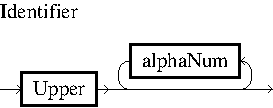
\includegraphics{bilder/Identifier}
\end{center}
\end{figure}

The reserved names are words that are not allows to occur as name of
an type expression. %
Our parser also knows the binary operations \ensuremath{\Conid{AND}}, \ensuremath{\Conid{NOT}} and \ensuremath{\Conid{OR}} and
since they are starting with an upper character, they are potential
type expressions. %
Therefore we need the parser to fail on these reserved names when
parsing type signatures. %

\begin{hscode}\SaveRestoreHook
\column{B}{@{}>{\hspre}l<{\hspost}@{}}%
\column{E}{@{}>{\hspre}l<{\hspost}@{}}%
\>[B]{}\Varid{specifierTokenParser}\mathrel{=}\Varid{makeTokenParser}\;\Varid{specifierDef}{}\<[E]%
\ColumnHook
\end{hscode}\resethooks

All parser the definitions generates are lexical parser, which means
they handle surrounding white spaces. % 
Hence, we do not need to consider white spaces, if we use one the
these parsers. %
As example, we get the parser that handles identifiers according to the defined
language. %

\begin{hscode}\SaveRestoreHook
\column{B}{@{}>{\hspre}l<{\hspost}@{}}%
\column{E}{@{}>{\hspre}l<{\hspost}@{}}%
\>[B]{}\Varid{sigIdentifier}\mathrel{=}\Varid{identifier}\;\Varid{signatureTokenParser}{}\<[E]%
\ColumnHook
\end{hscode}\resethooks

Other lexical parser we will use in our code includes \ensuremath{\Varid{whitespace}},
\ensuremath{\Varid{aSymbol}} and \ensuremath{\Varid{lexemer}}, where the latter takes a parser as argument
and parses trailing white spaces; \ensuremath{\Varid{aSymbol}} does the same, but
takes a string as argument.%
Additionally, we have parsers \ensuremath{\Varid{paren}} and \ensuremath{\Varid{bracket}} for parentheses
and brackets. %

Before we examine the first substructure, we need to consider the type
of our parser. %
We are parsing a \ensuremath{\Conid{String}} into a \ensuremath{\Conid{TypeExpr}}, thus, in the definitions
we used above, the type of our parser corresponds to: %

\begin{hscode}\SaveRestoreHook
\column{B}{@{}>{\hspre}l<{\hspost}@{}}%
\column{E}{@{}>{\hspre}l<{\hspost}@{}}%
\>[B]{}\Conid{TypeExprParser}\mathrel{=}\Conid{Parser}\;\Conid{String}\;\Conid{TypeExpr}{}\<[E]%
\ColumnHook
\end{hscode}\resethooks

In contrary to the parser structure we presented above, Parsec does
not return a list of possible results. % 
The data structure follows a different approach to determine if the
parser application was successful or not. % 
In the end, on success, the parser returns the longest possible
match. %

The first substructures we want to parse are type variables and
primitive types. %
Therefore, we first take a look at the following rail-road diagram,
where we illustrate the schema of the parser. %

\begin{figure}[h!]
\begin{center}
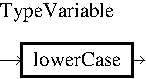
\includegraphics{bilder/TypeVariable}
\end{center}
\end{figure}

A type variables is one lower-case character. %

\begin{hscode}\SaveRestoreHook
\column{B}{@{}>{\hspre}l<{\hspost}@{}}%
\column{3}{@{}>{\hspre}l<{\hspost}@{}}%
\column{E}{@{}>{\hspre}l<{\hspost}@{}}%
\>[B]{}\Varid{varParser}\mathbin{::}\Conid{TypeExprParser}{}\<[E]%
\\
\>[B]{}\Varid{varParser}\mathrel{=}{}\<[E]%
\\
\>[B]{}\hsindent{3}{}\<[3]%
\>[3]{}\Varid{var}~\circledS~\Varid{lower}<\!\!\!*~\Varid{notFollowedBy}\;\Varid{alphaNum}){}\<[E]%
\ColumnHook
\end{hscode}\resethooks

Thus, we do not allow type variables like \ensuremath{\Conid{IO}\;\Varid{abc}}, \ensuremath{\Varid{varParser}} fails
on \ensuremath{\Varid{abc}} and our signature parser only reads \ensuremath{\Conid{IO}} as primitive type. %
After parsing, the function \ensuremath{\Varid{var}} converts the character into a
\ensuremath{\Conid{TypeExpr}}\footnote{\ensuremath{\Varid{a}} => \ensuremath{\Conid{TVar}\;\mathrm{97}}}. %
At the beginning, we followed the idea to parse one character only and
discard the rest, i.e., \ensuremath{\Conid{IO}\;\Varid{abc}} will be parsed as \ensuremath{\Conid{IO}\;\Varid{a}}, but
eventually decided against this concept. %
Later, we discuss this decision in more detail. %
% Type variables alone will not be parsed without the context of
% signatures (|":signature"|), because i

% If we parse type variables as part of a list or tuple, we need a
% slight change in our definition. %
% We still parse one lower-case character, but a type variable can
% appear in the middle of a tuple like |(Int, a, Int)| and hence, the
% type variables is followed by a semicolon. %
% The same reason applies for a type variable at the of a tuple or in a
% list, since we have to parse the closing bracket and parenthesis
% respectively. %
% Therefore, we only forbid another identifier to appear after a type
% variable in a list or tuple. %

The next parser handles primitive types like \ensuremath{\Conid{Int}} and \ensuremath{\Conid{Bool}},
but also the unit type \ensuremath{()}. 

\begin{figure}[h!]
\begin{center}
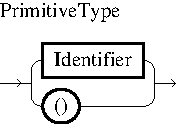
\includegraphics{bilder/PrimitiveType}
\end{center}
\end{figure}

For primitive types we need to parse one identifier and consider the
unit type \ensuremath{()} as special constructor. %

\begin{hscode}\SaveRestoreHook
\column{B}{@{}>{\hspre}l<{\hspost}@{}}%
\column{3}{@{}>{\hspre}l<{\hspost}@{}}%
\column{13}{@{}>{\hspre}l<{\hspost}@{}}%
\column{E}{@{}>{\hspre}l<{\hspost}@{}}%
\>[B]{}\Varid{primParser}\mathbin{::}\Conid{TypeExprParser}{}\<[E]%
\\
\>[B]{}\Varid{primParser}\mathrel{=}{}\<[E]%
\\
\>[B]{}\hsindent{3}{}\<[3]%
\>[3]{}\Varid{prim}~\circledS~(\Varid{sigIdentifier}{}\<[E]%
\\
\>[B]{}\Varid{x}{}\<[13]%
\>[13]{}~\rotatebox[origin=c]{90}{$\ominus$}~\Varid{aSymbol}\;\text{\tt \char34 ()\char34}){}\<[E]%
\ColumnHook
\end{hscode}\resethooks

The function \ensuremath{\Varid{prim}} wraps this identifier into a \ensuremath{\Conid{TCons}}-structure
with no type arguments\footnote{A little reminder: \ensuremath{\Conid{Int}} => \ensuremath{\Conid{TCons}\;(\text{\tt \char34 Prelude\char34},\text{\tt \char34 Int\char34})\;[\mskip1.5mu \mskip1.5mu]}}. %

In case of a n-ary type constructor, we parse at least one identifier
a white space and another type expression. %
At first, we parse an identifier like we do for primitive types and
additionally, we need a white space and another type expression to
follow. %

\begin{hscode}\SaveRestoreHook
\column{B}{@{}>{\hspre}l<{\hspost}@{}}%
\column{4}{@{}>{\hspre}l<{\hspost}@{}}%
\column{E}{@{}>{\hspre}l<{\hspost}@{}}%
\>[B]{}\Varid{consParser}\mathbin{::}\Conid{TypeExprParser}{}\<[E]%
\\
\>[B]{}\Varid{consParser}\mathrel{=}{}\<[E]%
\\
\>[B]{}\Varid{a}\;{}\<[4]%
\>[4]{}((\lambda \Varid{constr}\;\anonymous \;\Varid{expr}\to \Varid{cons}\;\Varid{constr}\;\Varid{expr}){}\<[E]%
\\
\>[4]{}~\circledS~\Varid{sigIdentifier}{}\<[E]%
\\
\>[4]{}\circledast\Varid{whitespace}{}\<[E]%
\\
\>[4]{}\circledast\Varid{sepBy1}\;(\Varid{signatureTerm}\;\Conid{False})\;\Varid{whitespace}){}\<[E]%
\ColumnHook
\end{hscode}\resethooks

The function \ensuremath{\Varid{sebBy1}} takes two parsers as arguments, where the second
parser is a separator that occurs between two tokens of the same
kind. %
At least one type signature (but no white space) needs to occur,
otherwise the parser \ensuremath{\Varid{sepBy1}} fails and altogether \ensuremath{\Varid{consParser}}
fails. %
Thus, in our case we parse at least two type expressions separated by
a white space or just one type expression. %
The parser \ensuremath{\Varid{signatureTerm}} handles all the substructures we listed
above, except for function types, but we discuss this later. %
The boolean value indicates, if a constructor type may occur without
parentheses. %
In the defintion above, further constructor types are only allowed to
occur with parentheses. %
As example to assure the accuracy of this idea: \ensuremath{\Conid{IO}\;\Varid{a}} and \ensuremath{\Conid{Maybe}\;\Varid{a}}
are type constructors with one type argument. If we combine these type
constructors to one expression, we get \ensuremath{\Conid{Maybe}\;(\Conid{IO}\;\Varid{a})} or \ensuremath{\Conid{IO}\;(\Conid{Maybe}\;\Varid{a})}. %
We have to parenthesize the inner type constructor because otherwise
\ensuremath{\Conid{IO}\;\Conid{Maybe}\;\Varid{a}} and \ensuremath{\Conid{Maybe}\;\Conid{IO}\;\Varid{a}} suggest that both constructors take two
type arguments instead of one. %
For a better unstanding, the following figures illustrate the idea of
this parser. %

\todo{constructor type does not fit here well}
\begin{figure}[h!]
\begin{center}
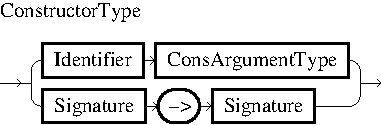
\includegraphics{bilder/ConstructorType}
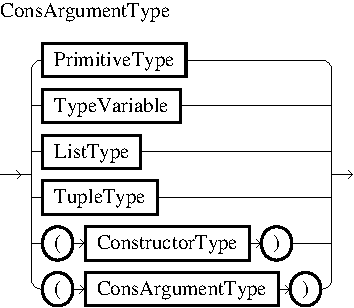
\includegraphics{bilder/ConsArgumentType}
\end{center}
\end{figure}


Next, let's take a look at the parsers for lists an tuples. %

\begin{figure}[h!]
\begin{center}
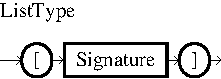
\includegraphics{bilder/ListType}
\end{center}
\end{figure}

The parser for lists is pretty simple, since a list can be any valid
type signature between brackets. %

\begin{hscode}\SaveRestoreHook
\column{B}{@{}>{\hspre}l<{\hspost}@{}}%
\column{3}{@{}>{\hspre}l<{\hspost}@{}}%
\column{E}{@{}>{\hspre}l<{\hspost}@{}}%
\>[B]{}\Varid{listParser}\mathbin{::}\Conid{TypeExprParser}{}\<[E]%
\\
\>[B]{}\Varid{listParser}\mathrel{=}{}\<[E]%
\\
\>[B]{}\hsindent{3}{}\<[3]%
\>[3]{}(\lambda \Varid{texpr}\to \Varid{cons}\;\text{\tt \char34 []\char34}\;[\mskip1.5mu \Varid{texpr}\mskip1.5mu])~\circledS~\Varid{bracket}\;(\Varid{signatureParser}\;\Conid{True}){}\<[E]%
\ColumnHook
\end{hscode}\resethooks

In the end, we wrap the result in a type constructor with \ensuremath{[\mskip1.5mu \mskip1.5mu]} as
constructor and the type signature as type arguments. %
Whereas \ensuremath{\Varid{signatureTerm}} is the parser for any type expression besides
function types, \ensuremath{\Varid{signatureParser}} parses the type signatures
altogether. %
The boolean value indicates again, if a constructor type may appear
without surrounding parentheses. %

Next, we present the parser for tuples in three steps.

\begin{figure}[h!]
\begin{center}
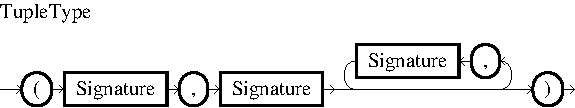
\includegraphics{bilder/TupleType}
\end{center}
\end{figure}
The first (and main) part looks similiar to the constructor parser. %
Only this time we parse any kind of type expressions seperated by a
comma instead of a white space. %

\begin{hscode}\SaveRestoreHook
\column{B}{@{}>{\hspre}l<{\hspost}@{}}%
\column{3}{@{}>{\hspre}l<{\hspost}@{}}%
\column{4}{@{}>{\hspre}l<{\hspost}@{}}%
\column{13}{@{}>{\hspre}c<{\hspost}@{}}%
\column{13E}{@{}l@{}}%
\column{E}{@{}>{\hspre}l<{\hspost}@{}}%
\>[B]{}\Varid{parseTuple}{}\<[13]%
\>[13]{}\mathrel{=}{}\<[13E]%
\\
\>[B]{}\hsindent{3}{}\<[3]%
\>[3]{}(\lambda \Varid{item}\;\anonymous \;\Varid{itemList}\to \Varid{item}\mathbin{:}\Varid{itemList})~\circledS~{}\<[E]%
\\
\>[3]{}\hsindent{1}{}\<[4]%
\>[4]{}(\Varid{signatureParser}\;\Conid{True}){}\<[E]%
\\
\>[3]{}\hsindent{1}{}\<[4]%
\>[4]{}\circledast\Varid{aSymbol}\;\text{\tt \char34 ,\char34}{}\<[E]%
\\
\>[3]{}\hsindent{1}{}\<[4]%
\>[4]{}\circledast\Varid{sepBy1}\;(\Varid{signatureParser}\;\Conid{True})\;(\Varid{aSymbol}\;\text{\tt \char34 ,\char34}){}\<[E]%
\ColumnHook
\end{hscode}\resethooks

We combine the first type expressions and the list of following type
expression to a list. %
This list represents the type arguments for the tuple constructor. %
Next, we need to build the tuple constructor because it depends on
the number of arguments: \ensuremath{(,)} is a tuple constructor for a pair,
whereas for a triple we need \ensuremath{(,,,)}. %

\begin{hscode}\SaveRestoreHook
\column{B}{@{}>{\hspre}l<{\hspost}@{}}%
\column{17}{@{}>{\hspre}l<{\hspost}@{}}%
\column{E}{@{}>{\hspre}l<{\hspost}@{}}%
\>[B]{}\Varid{tupleCons}\;\Varid{list}{}\<[17]%
\>[17]{}\mathrel{=}\text{\tt \char34 (\char34}\plus \Varid{replicate}\;(\Varid{length}\;\Varid{list}\mathbin{-}\mathrm{1})\;\text{\tt ','}\plus \text{\tt \char34 )\char34}{}\<[E]%
\ColumnHook
\end{hscode}\resethooks

Thus, depending on the list of type arguments, we construct the tuple
constructor. %
And in the end, we combine these functions to gain a parser for
tuples: %

\begin{hscode}\SaveRestoreHook
\column{B}{@{}>{\hspre}l<{\hspost}@{}}%
\column{3}{@{}>{\hspre}l<{\hspost}@{}}%
\column{5}{@{}>{\hspre}l<{\hspost}@{}}%
\column{E}{@{}>{\hspre}l<{\hspost}@{}}%
\>[B]{}\Varid{tupleParser}\mathbin{::}\Conid{TypeExprParser}{}\<[E]%
\\
\>[B]{}\Varid{tupleParser}\mathrel{=}{}\<[E]%
\\
\>[B]{}\hsindent{3}{}\<[3]%
\>[3]{}((\lambda \Varid{tuple}\to \Varid{cons}\;(\Varid{tupleCons}\;\Varid{tuple})\;\Varid{tuple}){}\<[E]%
\\
\>[3]{}\hsindent{2}{}\<[5]%
\>[5]{}~\circledS~\Varid{paren}\;\Varid{parseTuple}){}\<[E]%
\ColumnHook
\end{hscode}\resethooks
     
The last parser we need to discuss handles function types like \ensuremath{\Conid{Int}\to \Conid{Int}}. %
For an infix operator, we always need to look ahead after parsing an
identifier, if we come across the \ensuremath{\to }-operator next. %
Luckily, the Parsec library provides a mechanism to relieve us of
parsing operators. %

At first, we define the affix and associativity of the operator and
assign a function that determines the result of the parsing. %

\begin{hscode}\SaveRestoreHook
\column{B}{@{}>{\hspre}l<{\hspost}@{}}%
\column{3}{@{}>{\hspre}l<{\hspost}@{}}%
\column{E}{@{}>{\hspre}l<{\hspost}@{}}%
\>[B]{}\Varid{signatureTable}\mathrel{=}{}\<[E]%
\\
\>[B]{}\hsindent{3}{}\<[3]%
\>[3]{}[\mskip1.5mu [\mskip1.5mu \Conid{Infix}\;((\lambda \anonymous \to \Conid{FuncType})~\circledS~(\Varid{aSymbol}\;\text{\tt \char34 ->\char34}\;\Varid{x}))\;\Conid{AssocRight}\mskip1.5mu]\mskip1.5mu]{}\<[E]%
\ColumnHook
\end{hscode}\resethooks

Thus, when parsing a function arrow \ensuremath{\to } in an infix position, we
return the partial application of \ensuremath{\Conid{FuncType}} because the two
arguments of this constructor are the type expression to the left and
right of the operator\footnote{\ensuremath{\Conid{Int}\to \Conid{Int}} => \ensuremath{\Conid{FuncType}\;(\Conid{TCons}\;(\text{\tt \char34 \char34},\text{\tt \char34 Int\char34})\;[\mskip1.5mu \mskip1.5mu])\;(\Conid{TCons}\;(\text{\tt \char34 \char34},\text{\tt \char34 Int\char34})\;[\mskip1.5mu \mskip1.5mu]}}. %

In order to use this parser, we use Parsec's function
\ensuremath{\Varid{buildExpressionParser}} that takes such an definition table and
another parser to combine the two oft them. %

\begin{hscode}\SaveRestoreHook
\column{B}{@{}>{\hspre}l<{\hspost}@{}}%
\column{3}{@{}>{\hspre}l<{\hspost}@{}}%
\column{E}{@{}>{\hspre}l<{\hspost}@{}}%
\>[B]{}\Varid{signatureParser}\mathbin{::}\Conid{Bool}\to \Conid{TypeExprParser}{}\<[E]%
\\
\>[B]{}\Varid{signatureParser}\;\Varid{inAListOrTuple}\mathrel{=}{}\<[E]%
\\
\>[B]{}\hsindent{3}{}\<[3]%
\>[3]{}\Varid{buildExpressionParser}\;\Varid{signatureTable}\;(\Varid{signatureTerm}\;\Conid{True}\;\Varid{inAListOrTuple}){}\<[E]%
\ColumnHook
\end{hscode}\resethooks

The other parser that we assign is \ensuremath{\Varid{signatureTerm}}. %
We need to parametrize \ensuremath{\Varid{signatureParser}} as well, in order to indicate if we are
in the process of parsing a tuple or list. %
A list or a tuple can consist of function types without parentheses,
whereas for a valid constructor type, a function type as arguments
needs to be parenthesized. %
Additionally, we want to parse redundant parenthesized signatures as
well. %
We can offer this functionality with the following definition of
signatureTerm:

\begin{hscode}\SaveRestoreHook
\column{B}{@{}>{\hspre}l<{\hspost}@{}}%
\column{3}{@{}>{\hspre}l<{\hspost}@{}}%
\column{E}{@{}>{\hspre}l<{\hspost}@{}}%
\>[B]{}\Varid{signatureTerm}\mathbin{::}\Conid{Bool}\to \Conid{Bool}\to \Conid{TypeExprParser}{}\<[E]%
\\
\>[B]{}\Varid{signatureTerm}\;\Varid{allowConsParser}\;\Varid{inAListOrTuple}\mathrel{=}{}\<[E]%
\\
\>[B]{}\hsindent{3}{}\<[3]%
\>[3]{}(\Varid{guard}\;\Varid{allowConsParser}\sequ \Varid{try}\;\Varid{consParser}){}\<[E]%
\\
\>[B]{}\hsindent{3}{}\<[3]%
\>[3]{}~\rotatebox[origin=c]{90}{$\ominus$}~\Varid{try}\;\Varid{tupleParser}{}\<[E]%
\\
\>[B]{}\hsindent{3}{}\<[3]%
\>[3]{}~\rotatebox[origin=c]{90}{$\ominus$}~\Varid{paren}\;(\Varid{signatureParser}\;\Conid{False}){}\<[E]%
\\
\>[B]{}\hsindent{3}{}\<[3]%
\>[3]{}~\rotatebox[origin=c]{90}{$\ominus$}~\Varid{listParser}{}\<[E]%
\\
\>[B]{}\hsindent{3}{}\<[3]%
\>[3]{}~\rotatebox[origin=c]{90}{$\ominus$}~\Varid{primParser}{}\<[E]%
\\
\>[B]{}\hsindent{3}{}\<[3]%
\>[3]{}~\rotatebox[origin=c]{90}{$\ominus$}~(\Varid{varParser}\;\Varid{inAListOrTuple}){}\<[E]%
\ColumnHook
\end{hscode}\resethooks

In order to guarantee that we can parse tuples, parenthesized function
types and redundant parentheses, we cannot parse any characters in
case \ensuremath{\Varid{tupleParser}} fails, otherwise the parser for parenthesized
expressions fails too. %
Therefore, we have to try \ensuremath{\Varid{tuplesParser}} first; if it fails, the
result is discarded and we can try for parenthesized expressions
next. %
We do not need a try for the parenthesized expression because there
are no other valid expressions that start with an opening parenthesis,
since we already ruled out the possibility of tuples. %
Therefore, the parser \ensuremath{\Varid{paren}\;(\Varid{signatureParser}\;\Conid{False})} either fails on
the first character of an input or parses a valid parenthesized
expression.\footnote{Here we only consider well-balanced parentheses
  and discuss the handling of incorrect user input later.} %
The same logic holds for the following parsers, since they all expect
different first characters. %
For lists, the first input character has to be an open bracket,
\ensuremath{\Varid{primParser}} only accepts an upper-case character and \ensuremath{\Varid{varParser}} the
opposite, a lower-case character. \\ %

In the end, the signature parser joins the group of parses for
specifiers (\textss{\ensuremath{\mathbin{:}\mathbf{module}\;\Conid{IO}}}, \textss{\ensuremath{\mathbin{:}\Varid{function}\;\Varid{map}}} etc.) and
binary operators (\ensuremath{\Conid{AND}}, \ensuremath{\Conid{OR}}, \ensuremath{\Conid{NOT}}). %

\begin{figure}[h!]
\begin{minipage}{0.85\textwidth}
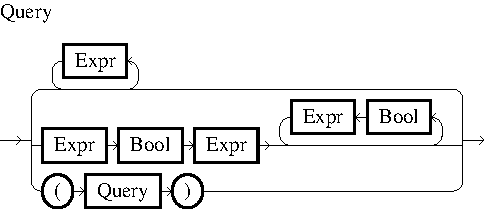
\includegraphics{bilder/Query}
\hspace{0.4cm}
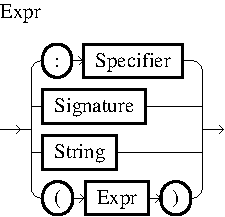
\includegraphics{bilder/Expr}
\end{minipage}
\hspace{-0.5cm}
\begin{minipage}{0.15\textwidth}
\vspace{-.7cm}
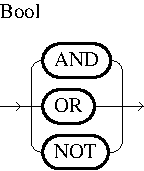
\includegraphics{bilder/Bool}
\end{minipage}
\end{figure}

Since we already parse any trailing white spaces, the actual parser
for queries we eventually call needs to parse all leading white
spaces. %
On the first layer, we apply the parser for the binary operations,
since we want to combine specifiers, signatures and pure search
terms. %
Under specification of several contexts and a pure search term without
any binary operations, the parser implicitly combines the
substructures with conjunctions, i.e., \textss{\ensuremath{\mathbin{:}\Varid{function}\;\Varid{map}\;\Varid{a}\to \Varid{b}}}
searches for a function starting with \emph{map}, which signature
consists of \ensuremath{\Varid{a}\to \Varid{b}}. %
The parser for signatures applies for the context of signatures, but
also for any word starting with an upper-case character that forms a
valid type expression and type signature respectively. %
This means, the search terms \textss{\ensuremath{\mathbin{:}\Varid{signature}\;\Varid{io}})} and
\textss{\ensuremath{\Conid{IO}}} yield the same \ensuremath{\Conid{Query}}-structure, hence the same search
results. %
On the contrary, type variables alone are not parsed implicitly
because we also want to search for words without context, i.e., we
search without a context for any word starting with a lower-case
character. %
In addition to the EBNF we already mentioned in
\hyperref[analysis:parser]{the last chapter}, we also provide the
summarised figures of this chapter with the additional parsers that
represent the query parser altogether (see
\hyperref[a:railroad]{Appendix \ref{a:railroad}}). %
Additionally, the parser always tries to parse as much words and
characters respectively. %
For example, if a valid expression is followed by nonsense, we parse
the first part and discard the other, i.e., \textss{\ensuremath{\Conid{IO}\;\mathrm{1}\;\anonymous \mathbin{!@\#\char94 }}}
yields the same results as \textss{\ensuremath{\Conid{IO}}}. %
And, as a last resort, we parse unbalanced parentheses that occur in
the beginning or end of the search term. %
We expect an intuitiv usage of the search engine of this underlying
parser and all the features the parser provides. %


% Give a definition of the language (EBNF(?) / appendix). 


%  query ::= expr [ expr ] | expr bool expr | (expr)
%  expr ::= (expr) | specifier | signature | string
%  bool ::= "AND" | "OR" | "NOT" 
%  specifier ::=  ":module" [ alphaNum ] | ":signature"  [ signature ]
%  |  ":function" [ alphaNum ] | ":flexible" | ":rigid" |  ":nondet" | ":det" 
%  signature ::= Upper alphaNum | function | constructor 
%  function ::= signature "->" signature  | lower "->" signature |
%  signature "->" lower
%  constructor ::= Upper alphaNum signature | Upper alphaNum lower
\chapter{Conclusion}\label{conclusion}

In the last chapter of this thesis, we complete this thesis with a
conclusion. %
At first, we review the progress of our implementation and tie in with
our introduction and the goals, requirements and ideas we had in the
beginning, respectively. %
Furthermore, we give an insight about lessons we learned and provide
an overview of ideas for future works. %

\section{Summary and Results}

The main goal was to build a search engine for the functional logic
programming language Curry in order to provide a simple way to look up
functions, modules and data types of Curry libraries, e.g.,
the libraries distributed with PAKCS. %
Therefore, we presented the CurryDoc tool to generate informative
documentations for a given Curry program. %
In \hyperref[implementation:currydoc]{chapter
  \ref{implementation:currydoc}} we demonstrated an extension of
CurryDoc in order to create a source of our information of Curry
libraries. %
This source produces a data structure that represents the given Curry
program that is eventually analysed in
\hyperref[implementation:index]{the following section} in order to
create an index for the search engine. %
The index consists of the data we want to search for, i.e., in our
case the API of the mentioned Curry libraries. %
The data we are indexing can be paired with a \textss{context} or,
more precisely, every information we are indexing is categorized
corresponding to its \textss{role} in the Curry program, e.g., a
function's name, the description of the module, a data type's
signature. %
These pairs of context and word allow us to improve our search engine
because we can restrict a search term to one of these contexts. %
This restrictions can minimize unwanted results and, therefore, make a
contribution to a user-friendly search engine. %
In order to provide the usage of such specifiers to restrict a search
term, we need a non-ambiguous language for the search queries. %
Therefore, we present a parser to analyze the search term in
\hyperref[implementation:parser]{the last section of chapter
  \ref{implementation}}. %
In the end, we have build a search engine to run as web
application. \\ %

In retrospective, we spent the most time studying the Holumbus
framework in detail and all the features it provides. %
After we consult the master's theses concerning the framework, the
main idea and general usage was clear pretty fast. %
Unfortunately, we discovered that these documentations of the
framework are quite out-of-date. %
Since the theses were written in 2008, the framework had many
improvements and new ideas were implemented. %
Thus, the fact, that it takes a lot of time to familiarise oneself
with an existing complex framework, was the first lesson that we
learned. %
However, after first approaches and a lot of time of progressive
implementation, we increased our knowledge of the structures that the
Holumbus framework provides. %
Eventually, we think that we interpenetrated how to use the framework
correctly. %
Furthermore, we entered a new field of analytics and semantics when we
studied the general idea of parser and eventually implemented our own
parser for the search queries. %
In this context, we used the Haskell library Parsec and had to
confront ourselves with a new complex library all over again. %
Fortunately, after a short time, we achieved good results and had
first successes with the implementation of our parser. %
In the end, it took several testing phases to pass all the
requirements and we often found improvements to simplify the
implementation but, all in all, we had very positive experiences with
Parsec and its functionality.\\ %

\todo[inline]{
  more?
}

\section{Outlook}

Last but not least, we want to discuss some ideas to extend this
project. %
One functionality we do not provide is an \emph{intelligent} way to
search for polymorphic types, like Hoogle, the search engine for
Haskell, does. %
For example, let's assume we search for a function that concatenates
two lists of integer. %
The best idea is to search for the signature of this function, i.e.,
\ensuremath{\text{\tt \char34 [Int]~->~[Int]\char34}}. %
Unfortunately, we will not find any results, since there is no
function with this specific type signature. %
But it exist a function to concatenate two lists of any type, i.e.,
\ensuremath{[\mskip1.5mu \Varid{a}\mskip1.5mu]\to [\mskip1.5mu \Varid{a}\mskip1.5mu]}. %
Like we mentioned, Hoogle uses a mechanism to search for more general
types in order to find the convenient function in our example. %
In our opinion, there is one simple approach to gain this
functionality and another one that requires more resources. %
The first approach just replaces each appearance of a type with a
fixed type variable. %
For our example, we can transform \ensuremath{[\mskip1.5mu \Conid{Int}\mskip1.5mu]\to [\mskip1.5mu \Conid{Int}\mskip1.5mu]} to \ensuremath{[\mskip1.5mu \Varid{a}\mskip1.5mu]\to [\mskip1.5mu \Varid{a}\mskip1.5mu]} if
we look at the first type \ensuremath{\Conid{Int}} and replace this and all following
occurrences with the type variable \ensuremath{\Varid{a}}. %
Another idea is to unify each type signature, that we have in the
index, with the searched signature and also return the successful
unifications. %
In the development period of this search engine, we simply did not
find the time to concern ourselves with this topic. %
Albeit, we think such a feature would be an excellent addition of the
already existing functionality. \\ %

Furthermore, we think that the widely-used "did you mean?" suggestion
can make our search engine even more user-friendly. %
In case of misspellings, this feature helps to find words that are
lexicographical similar with the search term in order to proceed the
search. %
The actual implementation will not be too complicated, since the
Holumbus framework already provides a fuzzy search that can help to
find the best result for misspelled words. \\ %

At last, we want to mention, that the interaction between the CurryDoc
extension and the Haskell implementation could be more modular. %
We tried to accomodate the search engine with the existing CurryDoc
and its function of generating documentation. %
For example, we compose the URI to provide the reference between a
result entry and the documentation in our search engine
implementation. %
Another approach would be to provide these kind of information in the
CurryDoc extension because, then, we can automatically consider
adjustments in the documentation process, like changes in the URI
construction. %
Another example can be the contexts; maybe a more flexible adjustment
of the context names is desirable. % 
One method could be to use construct the \ensuremath{\Conid{CurryInfo}} data structures
with several tuples, where the first entry represents the context and
the second entry the value. %
For example, \ensuremath{\Conid{ModuleInfo}} could look like this:

\begin{hscode}\SaveRestoreHook
\column{B}{@{}>{\hspre}l<{\hspost}@{}}%
\column{3}{@{}>{\hspre}l<{\hspost}@{}}%
\column{21}{@{}>{\hspre}l<{\hspost}@{}}%
\column{E}{@{}>{\hspre}l<{\hspost}@{}}%
\>[B]{}\mathbf{data}\;\Conid{ModuleInfo}\mathrel{=}{}\<[E]%
\\
\>[B]{}\hsindent{3}{}\<[3]%
\>[3]{}(\Conid{String},\Conid{String}){}\<[21]%
\>[21]{}\mbox{\onelinecomment  (context, name)}{}\<[E]%
\\
\>[B]{}\hsindent{3}{}\<[3]%
\>[3]{}(\Conid{String},\Conid{String}){}\<[21]%
\>[21]{}\mbox{\onelinecomment  (context, author)}{}\<[E]%
\\
\>[B]{}\hsindent{3}{}\<[3]%
\>[3]{}(\Conid{String},\Conid{String}){}\<[21]%
\>[21]{}\mbox{\onelinecomment  (context, description)}{}\<[E]%
\ColumnHook
\end{hscode}\resethooks

These are just some ideas we had in the end of our development. %
In the end, we had to differ between requirements and features and, of
course, we decided to focus on the requirements. %
We think, the features, that we just mentioned, are purely optional
and our search engine meets the requirements we made, provides a good
user-experience and is a good starting point for further
developments. %
During the implementation of the CurryDoc extension, we wanted to look
up a lot of functions and suffered from the lack of a
Hoogle-equivalent. %
We got really frustrated when browsing the online documentation and
reading each module in search of the convenient function. %
Hence, we hope to do some good with this search engine and help to
provide a more efficient work-environment for Curry. \\ %

\todo[inline]{something missing here?}


% Setze Numerierung wieder auf römisch zurück und setzte von oben fort
% Wert ist demnach der von 'roemisch'
\newpage
\pagenumbering{Roman}
\setcounter{page}{\value{roemisch}}

% Appendix, falls vorhanden
\appendix
\chapter{CurryDoc Instruction}\label{currydoc}
\section{Installation}

The installation requires a running Curry and curry2prolog system, we
recommend the PAKCS and
KICS2\footnote{\url{http://www-ps.informatik.uni-kiel.de/kics2/}}
implementation. \\

If you have a running Curry system, you can go on and modify the
included \emph{Makefile}. %
The first variable defines the path to your Curry implementation and
has to be modified. %
The following three stand for the provided libraries and the analysis
tool. %

\begin{tabbing}\tt
~CURRY\char61{}\char47{}path\char47{}to\char47{}your\char47{}CurryImplementation\\
\tt ~LIB\char61{}\char36{}\char123{}CURRY\char125{}\char47{}lib\\
\tt ~META\char61{}\char36{}\char123{}LIB\char125{}\char47{}meta\\
\tt ~ANADIR\char61{}\char36{}\char123{}CURRY\char125{}\char47{}tools\char47{}analysis
\end{tabbing}

The next path must link to the executable of your Curry implementation
and the last path must be modified to the directory of
the\emph{Makefile}.

\section{How-to-use}

You can either generate the \emph{.cdoc}-file itself or the HTML
representation, since the latter generates the \emph{.cdoc}-file as well.
 
\begin{tabbing}\tt
~\char36{}~currydoc~\char91{}\char45{}\char45{}nomarkdown\char93{}~\char91{}\char45{}\char45{}html\char124{}\char45{}\char45{}tex\char124{}\char45{}\char45{}cdoc\char93{}~\char60{}module\char95{}name\char62{}\\
\tt ~\char36{}~currydoc~\char91{}\char45{}\char45{}nomarkdown\char93{}~\char91{}\char45{}\char45{}html\char124{}\char45{}\char45{}tex\char124{}\char45{}\char45{}cdoc\char93{}~\\
\tt ~~~~\char60{}doc~directory\char62{}~\char60{}module\char95{}name\char62{}\\
\tt ~\char36{}~currydoc~\char91{}\char45{}\char45{}nomarkdown\char93{}~\char45{}\char45{}noindexhtml~\\
\tt ~~~~\char60{}doc~directory\char62{}~\char60{}module\char95{}name\char62{}\\
\tt ~\char36{}~currydoc~\char45{}\char45{}onlyindexhtml~\char60{}doc~directory\char62{}~\char60{}module\char95{}names\char62{}
\end{tabbing}

\chapter{Installation and Usage of Curr(y)gle}\label{currysearch}

\section{Installation}

This directory contains cabal-file, for the installation you simply
have to run cabal.

\begin{tabbing}\tt
~\char36{}~cabal~configure~\\
\tt ~\char36{}~cabal~build~\\
\tt ~\char36{}~cabal~install
\end{tabbing}

Alternatively you can use the provided \emph{Setup.hs}.
\begin{tabbing}\tt
~\char36{}~runhaskell~Setup\char46{}hs~configure\\
\tt ~\char36{}~runhaskell~Setup\char46{}hs~build\\
\tt ~\char36{}~runhaskell~Setup\char46{}hs~install
\end{tabbing}

\section{How-to-use}

The installation process creates to binaries: \emph{curryIndexer} and
\emph{curryServer}. %
The first creates the index for a given directory that contains at
least one \emph{.cdoc}-file and a corresponding URI. %
The \emph{.cdoc}-file can be generated with the extended CurryDoc for
a given Curry module, the URI is the corresponding HTML documentation
that also can be generated with CurryDoc. %
This package provides an example-directory with three Curry modules
generated with CurryDoc that provide some \emph{.cdoc}-files. %
So you can generate an index with these examples and the documentation
provided by PAKCS. %
The curryIndexer can either generate a new index or update the
existing one, to distinguish between these options, you can use the
flag \emph{- -n} for generating a new index and \emph{- -u} for
updating the index.

\begin{tabbing}\tt
~\char36{}~curryIndexer~\char46{}\char47{}example\char47{}CDOC\char95{}HTML~\\
\tt ~~~~http\char58{}\char47{}\char47{}www\char46{}informatik\char46{}uni\char45{}kiel\char46{}de\char47{}\char126{}pakcs\char47{}lib\char47{}CDOC\char47{}~\char45{}\char45{}n\\
\tt ~\char36{}~curryIndexer~\char46{}\char47{}example\char47{}CDOC\char95{}URL~\\
\tt ~~~~http\char58{}\char47{}\char47{}www\char46{}informatik\char46{}uni\char45{}kiel\char46{}de\char47{}\char126{}pakcs\char47{}lib\char47{}CDOC\char47{}~\char45{}\char45{}u\\
\tt ~\char36{}~curryIndexer~\char46{}\char47{}example\char47{}CDOC\char95{}XML~\\
\tt ~~~~http\char58{}\char47{}\char47{}www\char46{}informatik\char46{}uni\char45{}kiel\char46{}de\char47{}\char126{}pakcs\char47{}lib\char47{}CDOC\char47{}~\char45{}\char45{}u
\end{tabbing}

Since it can take a very long time to add each single module, you can
pass a \emph{.txt}-file as argument that consists of pairs of \emph{.cdoc-file} and
URI to generate the index.

\begin{tabbing}\tt
~\char36{}~curryIndexer~\char46{}\char47{}example\char47{}test\char46{}txt~\char45{}\char45{}n
\end{tabbing}

If you have generated an index, you can run the web application on your
localhost on a given port with the curryServer.

\begin{tabbing}\tt
~\char36{}~curryServer~\char45{}p~1337
\end{tabbing}

\chapter{User-Query Syntax}\label{syntax}

\section{EBNF}\label{a:ebnf}
\begin{hscode}\SaveRestoreHook
\column{B}{@{}>{\hspre}l<{\hspost}@{}}%
\column{27}{@{}>{\hspre}l<{\hspost}@{}}%
\column{29}{@{}>{\hspre}l<{\hspost}@{}}%
\column{E}{@{}>{\hspre}l<{\hspost}@{}}%
\>[B]{}\Conid{Query}{}\<[27]%
\>[27]{}\mathbin{::=}\{\mskip1.5mu \Conid{Expr}\mskip1.5mu\}\mid \Conid{Expr}\;\Conid{Bool}\;\Conid{Expr}\;\{\mskip1.5mu \Conid{Bool}\;\Conid{Expr}\mskip1.5mu\}\mid \text{\tt \char34 (\char34}\;\Conid{Query}\;\text{\tt \char34 )\char34};{}\<[E]%
\\
\>[B]{}\Conid{Expr}{}\<[27]%
\>[27]{}\mathbin{::=}\text{\tt \char34 :\char34}\;\Conid{Specifier}\mid \Conid{Signature}\mid \Conid{String}\mid \text{\tt \char34 (\char34}\;\Conid{Expr}\;\text{\tt \char34 )\char34};{}\<[E]%
\\
\>[B]{}\Conid{Bool}{}\<[27]%
\>[27]{}\mathbin{::=}\text{\tt \char34 AND\char34}\mid \text{\tt \char34 OR\char34}\mid \text{\tt \char34 NOT\char34};{}\<[E]%
\\
\>[B]{}\Conid{String}{}\<[27]%
\>[27]{}\mathbin{::=}\Conid{IdentStart}\;\{\mskip1.5mu \Conid{IdentLetter}\mskip1.5mu\}\mid \{\mskip1.5mu \Conid{Operator}\mskip1.5mu\};{}\<[E]%
\\
\>[B]{}\Conid{IdentStart}{}\<[27]%
\>[27]{}\mathbin{::=}\text{\tt \char34 \char95 \char34}\mid \Varid{lower};{}\<[E]%
\\
\>[B]{}\Conid{IdentLetter}{}\<[27]%
\>[27]{}\mathbin{::=}\Varid{alphaNum}\mid \text{\tt \char34 '\char34};{}\<[E]%
\\
\>[B]{}\Conid{Operator}{}\<[27]%
\>[27]{}\mathbin{::=}\text{\tt \char34 :\char34}\mid \text{\tt \char34 !\char34}\mid \text{\tt \char34 \#\char34}\mid \text{\tt \char34 \$\char34}\mid \text{\tt \char34 \%\char34}\mid \text{\tt \char34 \&\char34}\mid \text{\tt \char34 *\char34}\mid \text{\tt \char34 +\char34}\mid \text{\tt \char34 .\char34}{}\<[E]%
\\
\>[27]{}\hsindent{2}{}\<[29]%
\>[29]{}\mid \text{\tt \char34 /\char34}\mid \text{\tt \char34 <\char34}\mid \text{\tt \char34 /\char34}\mid \text{\tt \char34 <\char34}\mid \text{\tt \char34 =\char34}\mid \text{\tt \char34 >\char34}\mid \text{\tt \char34 ?\char34}\mid \text{\tt \char34 @\char34}\mid \text{\tt \char34 \char92 \char92 \char34}{}\<[E]%
\\
\>[27]{}\hsindent{2}{}\<[29]%
\>[29]{}\mid \text{\tt \char34 \char94 \char34}\mid \text{\tt \char34 |\char34}\mid \text{\tt \char34 -\char34}\mid \text{\tt \char34 \char126 \char34}\mid \text{\tt \char34 \char95 \char34};{}\<[E]%
\\
\>[B]{}\Conid{Signature}{}\<[27]%
\>[27]{}\mathbin{::=}\Conid{ConstructorType}\mid \Conid{ConsArgumentType};{}\<[E]%
\\[\blanklineskip]%
\>[B]{}\Conid{ConstructorType}{}\<[27]%
\>[27]{}\mathbin{::=}\Conid{Identifier}\;\Conid{ConsArgumentType}\mid \Conid{Signature}\;\text{\tt \char34 ->\char34}\;\Conid{Signature};{}\<[E]%
\\
\>[B]{}\Conid{ConsArgumentType}{}\<[27]%
\>[27]{}\mathbin{::=}\Conid{PrimitiveType}\mid \Conid{TypeVariable}\mid \Conid{ListType}\mid \Conid{TupleType}{}\<[E]%
\\
\>[27]{}\hsindent{2}{}\<[29]%
\>[29]{}\mid \text{\tt \char34 (\char34}\;\Conid{ConstructorType}\;\text{\tt \char34 )\char34}\mid \text{\tt \char34 (\char34}\;\Conid{ConsArgumentType}\;\text{\tt \char34 )\char34};{}\<[E]%
\\
\>[B]{}\Conid{ListType}{}\<[27]%
\>[27]{}\mathbin{::=}\text{\tt \char34 [\char34}\;\Conid{Signature}\;\text{\tt \char34 ]\char34};{}\<[E]%
\\
\>[B]{}\Conid{TupleType}{}\<[27]%
\>[27]{}\mathbin{::=}\text{\tt \char34 (\char34}\;\Conid{Signature}\;\text{\tt \char34 ,\char34}\;\Conid{Signature}\;\{\mskip1.5mu \text{\tt \char34 ,\char34}\;\Conid{Signature}\mskip1.5mu\}\;\text{\tt \char34 )\char34};{}\<[E]%
\\
\>[B]{}\Conid{PrimitiveType}{}\<[27]%
\>[27]{}\mathbin{::=}\Conid{Identifier}\mid \text{\tt \char34 ()\char34};{}\<[E]%
\\
\>[B]{}\Conid{TypeVariable}{}\<[27]%
\>[27]{}\mathbin{::=}\Varid{lowerCase};{}\<[E]%
\\
\>[B]{}\Conid{Identifier}{}\<[27]%
\>[27]{}\mathbin{::=}\Conid{Upper}\;\{\mskip1.5mu \Varid{alphaNum}\mskip1.5mu\};{}\<[E]%
\ColumnHook
\end{hscode}\resethooks

\begin{hscode}\SaveRestoreHook
\column{B}{@{}>{\hspre}l<{\hspost}@{}}%
\column{27}{@{}>{\hspre}l<{\hspost}@{}}%
\column{29}{@{}>{\hspre}l<{\hspost}@{}}%
\column{E}{@{}>{\hspre}l<{\hspost}@{}}%
\>[B]{}\Conid{Specifier}{}\<[27]%
\>[27]{}\mathbin{::=}\Conid{SignatureSpecifier}\mid \Conid{ModuleSpecifier}\mid \Conid{FunctionSpecifier}{}\<[E]%
\\
\>[27]{}\hsindent{2}{}\<[29]%
\>[29]{}\mid \Conid{TypeSpecifier}\mid \Conid{AuthorSpecifier}\mid \Conid{InModuleSpecifier}{}\<[E]%
\\
\>[27]{}\hsindent{2}{}\<[29]%
\>[29]{}\mid \Conid{FlexibleSpecifier}\mid \Conid{RigidSpecifier}{}\<[E]%
\\
\>[27]{}\hsindent{2}{}\<[29]%
\>[29]{}\mid \Conid{NonDetSpecifier}\mid \Conid{DetSpecifier};{}\<[E]%
\\
\>[B]{}\Conid{SignatureSpecifier}{}\<[27]%
\>[27]{}\mathbin{::=}\text{\tt \char34 signature\char34}\;[\mskip1.5mu \Conid{Signature}\mskip1.5mu]\mid \text{\tt \char34 s\char34}\;[\mskip1.5mu \Conid{Signature}\mskip1.5mu];{}\<[E]%
\\
\>[B]{}\Conid{ModuleSpecifier}{}\<[27]%
\>[27]{}\mathbin{::=}\text{\tt \char34 module\char34}\;[\mskip1.5mu \Varid{alphaNum}\mskip1.5mu]\mid \text{\tt \char34 m\char34}\;[\mskip1.5mu \Varid{alphaNum}\mskip1.5mu];{}\<[E]%
\\
\>[B]{}\Conid{FunctionSpecifier}{}\<[27]%
\>[27]{}\mathbin{::=}\text{\tt \char34 function\char34}\;[\mskip1.5mu \Varid{alphaNum}\mskip1.5mu]\mid \text{\tt \char34 f\char34}\;[\mskip1.5mu \Varid{alphaNum}\mskip1.5mu];{}\<[E]%
\\
\>[B]{}\Conid{TypeSpecifier}{}\<[27]%
\>[27]{}\mathbin{::=}\text{\tt \char34 type\char34}\;[\mskip1.5mu \Varid{alphaNum}\mskip1.5mu]\mid \text{\tt \char34 t\char34}\;[\mskip1.5mu \Varid{alphaNum}\mskip1.5mu];{}\<[E]%
\\
\>[B]{}\Conid{AuthorSpecifier}{}\<[27]%
\>[27]{}\mathbin{::=}\text{\tt \char34 author\char34}\;[\mskip1.5mu \Varid{alphaNum}\mskip1.5mu]\mid \text{\tt \char34 a\char34}\;[\mskip1.5mu \Varid{alphaNum}\mskip1.5mu];{}\<[E]%
\\
\>[B]{}\Conid{InModuleSpecifier}{}\<[27]%
\>[27]{}\mathbin{::=}\text{\tt \char34 inModule\char34}\;[\mskip1.5mu \Varid{alphaNum}\mskip1.5mu]\mid \text{\tt \char34 in\char34}\;[\mskip1.5mu \Varid{alphaNum}\mskip1.5mu];{}\<[E]%
\\
\>[B]{}\Conid{FlexibleSpecifier}{}\<[27]%
\>[27]{}\mathbin{::=}\text{\tt \char34 flexible\char34}\mid \text{\tt \char34 fl\char34};{}\<[E]%
\\
\>[B]{}\Conid{RigidSpecifier}{}\<[27]%
\>[27]{}\mathbin{::=}\text{\tt \char34 rigid\char34}\mid \text{\tt \char34 r\char34};{}\<[E]%
\\
\>[B]{}\Conid{NonDeterSpecifier}{}\<[27]%
\>[27]{}\mathbin{::=}\text{\tt \char34 nondet\char34}\mid \text{\tt \char34 nd\char34};{}\<[E]%
\\
\>[B]{}\Conid{DetSpecifier}{}\<[27]%
\>[27]{}\mathbin{::=}\text{\tt \char34 det\char34}\mid \text{\tt \char34 d\char34};{}\<[E]%
\ColumnHook
\end{hscode}\resethooks

\section{Rail-Road Diagram}\label{a:railroad}
\vspace{-0.6cm}
\begin{minipage}{0.85\textwidth}
\begin{minipage}{0.55\textwidth}
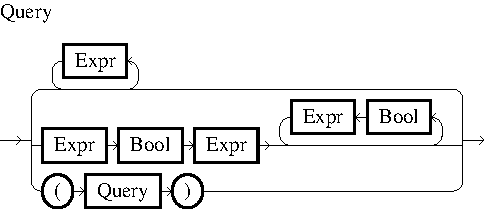
\includegraphics{bilder/Query}
\end{minipage}
\hspace{1.3cm}
\begin{minipage}{0.45\textwidth}
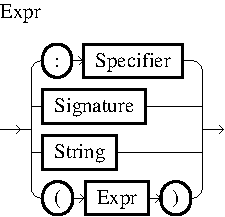
\includegraphics{bilder/Expr}
\end{minipage}

\begin{minipage}[t]{0.5\textwidth}
\vspace{1cm}

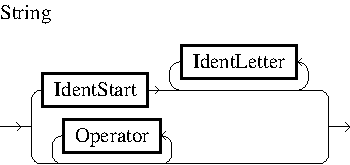
\includegraphics{bilder/String}

\vspace{1cm}
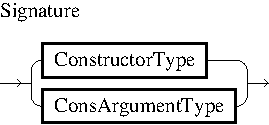
\includegraphics{bilder/Signature}

\vspace{1cm}
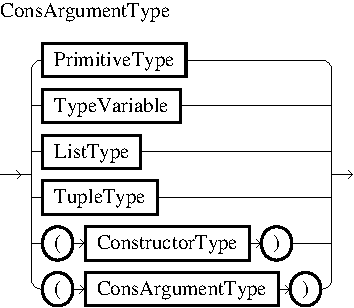
\includegraphics{bilder/ConsArgumentType} 

\end{minipage}
\begin{minipage}[t]{0.5\textwidth}

\vspace{1cm}

\includegraphics{bilder/identStart}
\includegraphics{bilder/identLetter}

\vspace{1.68cm}
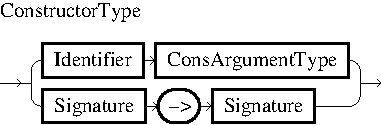
\includegraphics{bilder/ConstructorType}

\vspace{1cm}
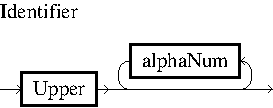
\includegraphics{bilder/Identifier}

\vspace{1cm}
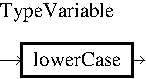
\includegraphics{bilder/TypeVariable}
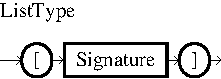
\includegraphics{bilder/ListType}
\end{minipage}

\vspace{0.5cm}
\begin{minipage}{0.5\textwidth}
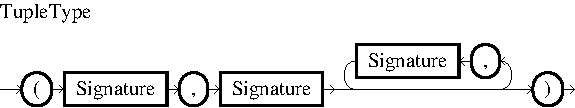
\includegraphics{bilder/TupleType}
\end{minipage}
\hspace{3.25cm}
\begin{minipage}{0.5\textwidth}
\vspace{0.25cm}
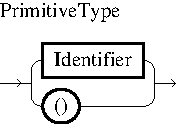
\includegraphics{bilder/PrimitiveType}
\end{minipage}

\end{minipage}
\begin{minipage}{0.15\textwidth}
\vspace{0.5cm}
{\hspace{-0.5cm}
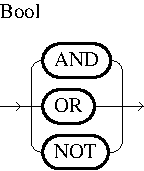
\includegraphics{bilder/Bool}}

\vspace{0.4cm}

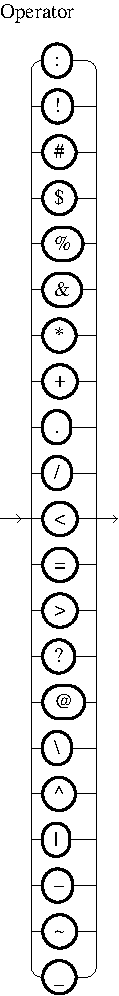
\includegraphics{bilder/Operator}
\end{minipage}

\begin{center}
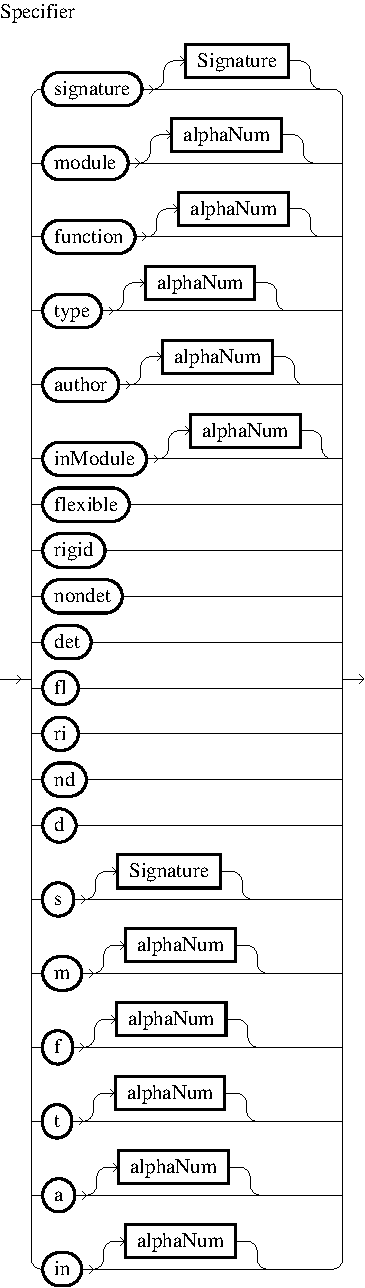
\includegraphics{bilder/Specifier}
\end{center}

% Literaturverzeichnis
\bibliography{literatur/bib}

% Eidesstattliche Erklärung
% \input{extras/eidesstattliche}

\end{document}
